\clearpage
\part*{Part VII. The Photon\\[5pt]{\large The (3,2) cell}}
\label{atlaspart:07-cell-3-2-photon}
\addcontentsline{toc}{part}{Part VII. The Photon, The (3,2) cell}
\section*{Introduction to Part VII}\label{narr:part:V}
\addcontentsline{toc}{section}{Introduction to Part VII}
Electrodynamics is where the construction first meets a number. The one link of the abelian genre carries a coupling, and the chapters of this Part read that coupling, the dipole factors of the charged leptons, the ladder of hydrogen, the Lamb and Casimir effects, the finiteness of the sums, the running of the coupling and the photon itself, all from the records a read leaves at the one link and the apparatus webs of chapter 1-6. The Part also carries the ladder of the charged leptons as hub assemblies, the face dissolution and the exponent, and the Koide class, which belong here because they are read at the same dock. Five results are theorems and the rest are conditional theorems or open results, the conditions listed in the boxes; no number taken from experiment enters any chapter.

The order of the twelve chapters is the order in which the objects are built. The coupling at the one link comes first because every other chapter reads something at that link or at a web docked to it. The dipole factors come next because they are the first readouts at an apparatus web, the anomaly web, with the measuring body in place. Hydrogen follows because the held carrier is the first closed read with a mass reading, and the Casimir count rests on hydrogen and the saturation. The two chapters on the sums explain why none of these readouts needs a subtraction, and the photon chapter and the empty Dirac chapter close the electrodynamic thread. The last three chapters turn from the one link to the three charged leptons as webs, and they are placed here rather than in Part X because the dock at which they are read is the electron dock of this Part. A reader who wants the single most important page of the Part should read chapter 5-6, where the finiteness of every sum is stated as a property of the grading by order.

Chapter 5-1 reads the fine-structure constant at the one link in Theorem~124.1, resting on the records, the probe, the state space, the probability rule, the order coordinate, the rotation group and spin. The derivation is stated at the twenty-eight statements of the alpha Letter and closed in the kernel at the machine-checked package of the one-link value theorem, so that this chapter states the result and its standing while the companion letter carries the replication, Theorem~124.1. Beside it stand the phase residue as the Ward gauge, Open result~125.1, an open result, the mass-chain premise census, Table~126.1, the alpha Letter, Table~127.1, which carries the replication of that constant in full, and the discrete laws as the reflections up to re-matching, Open result~128.1. The first of these is an open result a reader of gauge theory should read closely: the phase residue is not the Ward gauge at the register of the pair state, because the rephasing group of the Schmidt basis, the per-vector phases at the near end compensated at the far end direction by direction with the global phase factored out, is a lattice of rank two beyond the register scalars, while the one-parameter group of the letter generator is one scalar per end, traceless and fixed by every matching, Open result~125.1. The census beside it transcribes the condition union of the mass chain from its table of hypotheses and re-derives it from the chain results, equal at its four entries, the count of a read, the geodesic, the tie and the typing of the arm, each entry typed as discharged, named or owed, Table~126.1. A reader who wants the whole derivation of the constant reads the companion letter; this Part states the result and its standing.

Chapters 5-2 and 5-3 are the dipole chapters. Theorem~141.1 gives the electron dipole factor at order three from the self-terms, and the table of the chapter counted empty (in chapter~\ref{mod:II-10-decoherence-and-the-open-system}, among the instruments) records the muon chapter as counted empty. At the anomaly web with the measuring body in place the readout at order two equals the sum of the tabulated self-terms at all eight own-link records, and the order-three term is zero, the direct record sum graded by the surviving exchange count terminating, Theorem~141.1. The reader will notice that the vanishing of the third-order term is a statement about a finite sum and not about a cancellation among divergent integrals, which is the shape every result of this Part takes. Chapter 5-4 reads hydrogen from the held carrier, Theorem~143.1, with the hyperfine interval as the junction holonomy at the hydrogen sink, Open result~144.1, open beside it. Hydrogen is the held carrier in a literal sense: the photon word held at both ends, the qutrit end at the electron dock and the qubit end at the up core of the proton, is a closed read with a mass reading, and its level-one binding through the electron body is an exact element, Theorem~143.1. The open result beside it reads the twenty bound walks through the bond and the junction of the standing hydrogen sink and finds the identity on the qubit register at all sixty holonomies at the standing transport, the two orientations equal and the interval between the two reads the zero element, which is the parting, Open result~144.1. Chapter 5-5 reads the Casimir effect as the boundary count between two sinks, Theorem~145.1, which is a theorem: the excluded count between two sinks of the saturation placed along a chain is a definite function of the separation at every separation the chain admits, with one sign, the excluded records defined at all forty-four chains, so that the effect is a composed cell of the second-law and chain results, Theorem~145.1.

Chapters 5-6 and 5-7 concern the sums. Theorem~146.1 reads the ladder as the order grading of the finite record sum, which is the version of finiteness the construction gives without renormalization, and Theorem~147.1 reads the scale as the body at the carrier readouts, with the scale body as the joined apparatus web in Theorem~148.1. At the one link and at every one of the sixteen webs of the direct-sum result the record sum graded by order carries exactly the three rungs zero, one and two, the spacing of the ladder in the act count is one at every step, and the act count is the number operator, Theorem~146.1. There is therefore nothing to subtract: the sum has three rungs and stops. The four coupling readouts are defined through their carrier bodies at both port faces and both register faces, the direct sum through the body reproducing the readouts of the three results it rests on, so the scale is the body itself at its rest energy and no parameter, Theorem~147.1, and that body is the standing apparatus web joined to the one (2,3) link at its register, at every one of the three measurement webs of the matching column, Theorem~148.1. Chapter 5-8 reads the photon as docking at both faces in Theorem~150.1: the photon word, held at both of its ends under the docking act of the axiom text, the qutrit end at the electron dock and the qubit end at the up core by two qutrit-qubit pairs, docks at both of its faces, with pair production read at the join face, Theorem~150.1. Chapter 5-9 records the Dirac chapter as counted empty, at the table of the chapter counted empty (in chapter~\ref{mod:II-10-decoherence-and-the-open-system}, among the instruments), with the Dirac form at an established generator in the open result titled The Dirac form at an established generator commuting with the rest letter (in chapter~\ref{mod:V-9-D538654-w-fcgd}, among the instruments) as an open result: at the docked (2,3) link of the standing electron web the register six is the qubit factor multiplied by the qutrit factor and the rest letter is the lifted dock letter with the level, and among the established candidate generators none commutes with the rest letter, which is the parting, the open result titled The Dirac form at an established generator commuting with the rest letter (in chapter~\ref{mod:V-9-D538654-w-fcgd}, among the instruments).

The last three chapters read the charged leptons. Theorem~152.1 reads the lepton ladder as hub assemblies, Theorem~155.1 is the face dissolution theorem with the leg count and the exponent, and Open result~157.1 states the Koide relation at the dock unit as an open result. At every one of the three lepton webs the unstruck links are the three colored core links plus a number of hub assemblies, each one in-leg, three qubit-ququart legs and one qubit pair at the measure forty, the electron at one assembly, the muon at two and the tau at three, Theorem~152.1. The two readings of the mass law, the dock reading and the hub reading, are one law up to the unit absorbing one leg at every established result, the ratio form carries no reading, and the reading word is dissolved with its residue the leg function as a corollary, Theorem~155.1. At the dock spelling the Koide relation lies outside the field of the two roots at the direct-sum order, the three adjoined roots independent, so it equals two thirds in the field at no reading, the departure an exact object of the tower with the sign positive at the ladder of the construction and negative at the derived ladder, both faces printed, Open result~157.1. These three rest on the mass unit of chapter 8-1, which the reader meets again in Part X; the dependency lines beneath the boxes say so.

In the language of the literature, this Part names the fine-structure constant, the anomalous dipole factor, the Rydberg ladder, the fine and hyperfine structure, the Lamb shift, the Casimir effect, renormalization, the running coupling, the photon, pair production, the Dirac equation and the Koide relation. The correspondence is by name at each. The boxes establish counts and sums over finitely many records at the one link, and the register matrix of the framework chapter places the photon at the cell (2,3) as the first conjecture of the compendium.

The dependency lines of the Part reach into Parts I, III and IV and forward into Part X. The constant rests on the records and the probe of Part I, on the state space and the probability rule of Part III and on the order coordinate, the rotation group and spin of Part IV. The dipole factor rests on the records, the probe and the constant. Hydrogen rests on the held carrier and the constant, and the Casimir count on the records, the saturation and hydrogen. The photon chapter rests on the link, the moves, the saturation, the probe, the constant and hydrogen. The three lepton chapters rest on the moves, the saturation and the mass unit of chapter 8-1, so that a reader following the derivation graph meets the one forward edge of the Part there and can see that nothing of electrodynamics rests on it. The open questions of the Part are stated at its open results, the Ward gauge at the phase residue, the hyperfine interval at the junction holonomy, the Dirac form at a commuting generator and the Koide relation at the dock unit, and each box names the parting rather than leaving the reader to guess at it.
\section{The fine-structure constant at the one link: the infrared restatement with the Photon Conjecture}\label{mod:V-1-fine-structure-constant-at-the-one-link}
\chdesig{7-1}{5-1}{V-1-fine-structure-constant-at-the-one-link}{V-1-D543680-w-rmdf}
\par\noindent\fbox{\parbox{0.96\linewidth}{\small The canonical statement of this result is the Letter in \texttt{papers/alpha} of this repository, \emph{A Parameter-Free Candidate for the Fine-Structure Constant from Entangled Qudits}. Its five definitions, its read cap and its two exchanges supersede the wording of this chapter where the two differ, and its Lean check is the Letter's single file \texttt{papers/alpha/lean/ChainAlpha.lean}.}}\par\medskip
\label{narr:open:5-1}The first number of the compendium is read here. Theorem~124.1 reads the fine-structure constant at the one link, resting on the records, the probe, the state space, the probability rule, the order coordinate, the rotation group and spin. The phase residue as the Ward gauge, Open result~125.1, the mass-chain premise census, Table~126.1, the alpha Letter, Table~127.1, and the discrete laws as the reflections up to re-matching, Open result~128.1, stand beside it.
\begin{chconditional}[The fine-structure constant at the one link]\label{box:V-1-fine-structure-constant-at-the-one-link:1}
This result is conditional on the axiom text and on the results of the chapters named as its premises in the derivation below, each at its own standing.
The derivation is stated at the thirty-two numbered statements of the alpha Letter, twelve theorems, eleven lemmas, eight corollaries and one conjecture, and closed in the kernel at the Lean package of the one-link value theorem synced to that page at every label, number and title.\textsuperscript{,} The readable links with both ends of dimension at least two are the $(2,2)$ and $(2,3)$ types; the pair state is the one pure state fixed by the twirl and every readout the normalized trace against the pair projector; the $(2,3)$ link alone carries a central generator acting on its pair, abelian, conserved and massless, with two transverse states at its open read; the records of its two reads are 172, in four sectors of sizes 79, 48, 42 and 3 with the weights one, root two, root three and root six by the gain law; the readout algebra is the register 31104; and the two-point function is the sum of the record weights over the register,
\end{chconditional}
\chstanding{a conditional theorem}
\chdeps{the theorems of Chapters 1-0 to 1-3, 1-6, 3-1 to 3-2, 4-1 to 4-2, 4-5}{the theorems of Chapters 1-2, 1-4, 4-5 to 4-6, 5-11, 5-13, 5-16, 7-1 to 7-2, 7-4, 7-6 to 7-8}
\begin{equation}
\alpha(0) = \frac{79 + 48\sqrt{2} + 42\sqrt{3} + 3\sqrt{6}}{31104},
\label{eq:alpha}
\end{equation}
in exact arithmetic in $\mathbb{Q}(\sqrt{2},\sqrt{3})$, under the correspondence the fine-structure constant at zero momentum transfer, its digits printed at the standalone letter.
The two-point function factorizes as the bare unit, the generator factor and the residue, the matching relation of the on-shell scheme, each factor an output of the same computation. Every premise of the correspondence stands discharged in the kernel, the premise union empty at the page and at the eleventh Lean release alike, the premise census having typed the eight binders ahead of the discharges.
Fifteen further theorems re-meet the parts of the derivation, the letter-state residue, the closure records, the mixed half, the carrier root, the root-first trace, the closure clause and its sign, the configuration, the office at the one link, the Thomson-class corollary and the Lean derivations,\textsuperscript{,}\textsuperscript{,}\textsuperscript{,}\textsuperscript{,}\textsuperscript{,}\textsuperscript{,}\textsuperscript{,}\textsuperscript{,}\textsuperscript{,}\textsuperscript{,}\textsuperscript{,}\textsuperscript{,}\textsuperscript{,}\textsuperscript{,} and six supporting entries carry the replication pack, the single file and the alpha Letter.\textsuperscript{,}\textsuperscript{,}\textsuperscript{,}\textsuperscript{,}\textsuperscript{,}
Twelve open results stand here, at the carrier root and its placement, the witness weight, the configuration and its minimality, the centre-line form and normalisation, the two matchings, the fourth root and the inner-product phases, and the closure eigenvalue at the second route;\textsuperscript{,}\textsuperscript{,}\textsuperscript{,}\textsuperscript{,}\textsuperscript{,}\textsuperscript{,}\textsuperscript{,}\textsuperscript{,}\textsuperscript{,}\textsuperscript{,}\textsuperscript{,} four further entries placed here, the pole residue, the theta angle as the junction holonomy, the eleventh Lean release and its single file, are cited at their own standing.\textsuperscript{,}\textsuperscript{,}\textsuperscript{,}
\begin{chbridge}
The fine-structure constant $\alpha = e^{2}/4\pi\epsilon_{0}\hbar c$ is the dimensionless coupling of the electron to the electromagnetic field \cite{Sommerfeld1916}, in quantum electrodynamics the renormalized coupling at zero momentum transfer \cite{Peskin1995}; the Standard Model takes it from experiment, its recommended value printed by the adjustment of the constants \cite{Mohr2025} and displayed here by that citation alone. The correspondence is by name; the record supplies a step generator at the order coordinate, a first-power operator, a direction functional and an office at the common support carrying the energy, momentum and mass names at chapter~\ref{mod:I-3-records-reads-and-the-born-count-the-gain-lemma}, chapter~\ref{mod:I-6-read-at-a-register-the-probe-and-the-measurement}, chapter~\ref{mod:II-6-energy-and-the-hamiltonian-the-first-power-operator-and-the-step}, chapter~\ref{mod:III-1-order-coordinate-and-its-theorem}, chapter~\ref{mod:III-6-p-c-t-and-cpt}, chapter~\ref{mod:IV-6-conservation-as-the-kernel-of-the-move-matrix}, chapter~\ref{mod:V-7-running-of-the-coupling}, the chapter titled The Dirac equation at the dock (chapter~\ref{mod:V-9-dirac-equation-at-the-dock}, among the instruments), chapter~\ref{mod:VIII-1-mass-unit-and-the-first-power}, chapter~\ref{mod:VIII-5-unified-mass-readout}, chapter~\ref{mod:X-2-field-equation-at-the-counting-face}, the chapter titled The gravitational and cosmological constants table (chapter~\ref{mod:X-9-gravitational-and-cosmological-constants-table}, among the instruments), chapter~\ref{mod:XI-1-second-law-as-the-boundary-count-under-acts} and chapter~\ref{mod:XIV-7-what-remains-the-ungraded-page} and a joined saturation carrying the hydrogen name, a two-vertex term carrying the Rydberg name, cells at the hydrogen sink carrying the Lamb and hyperfine names, self-terms carrying the coupling names and joined electron sinks carrying the periodic-table name at chapter~\ref{mod:IV-8-ward-identity-and-the-anomaly-sums}, chapter~\ref{mod:V-2-electron-anomalous-dipole-factor-through-order-three}, the chapter titled The muon anomalous dipole factor (chapter~\ref{mod:V-3-muon-anomalous-dipole-factor}, among the instruments), chapter~\ref{mod:V-4-hydrogen-the-rydberg-ladder-and-the-fine-structure}, chapter~\ref{mod:V-5-lamb-shift-and-the-casimir-effect}, chapter~\ref{mod:V-8-photon-docking-the-join-face-and-pair-production}, the chapter titled The mesons and the nucleon at the cap (chapter~\ref{mod:VII-9-mesons-and-the-nucleon-at-the-cap}, among the instruments), chapter~\ref{mod:XII-3-chain-of-pairs-and-the-charged-periodic-sink}, chapter~\ref{mod:XII-5-periodic-table-as-the-joined-electron-sinks} and chapter~\ref{mod:XIV-7-what-remains-the-ungraded-page}, and the momentum, the energy, and the periodic table correspond there and here by name.
\end{chbridge}
\begin{chproof}[finite computation]
The premises of this derivation are the axiom and the six definitions of chapter~\ref{mod:FRAMEWORK}, the open result of chapter~\ref{mod:I-1-axiom-and-the-six-definitions}, the theorem of chapter~\ref{mod:I-2-link-and-its-six-genres}, the theorem of chapter~\ref{mod:I-3-records-reads-and-the-born-count-the-gain-lemma}, the theorem of chapter~\ref{mod:I-6-read-at-a-register-the-probe-and-the-measurement}, the theorem of chapter~\ref{mod:II-1-state-space-from-the-act-outputs}, the theorem of chapter~\ref{mod:II-2-born-rule-and-unitarity}, the theorem of chapter~\ref{mod:III-1-order-coordinate-and-its-theorem}, the theorem of chapter~\ref{mod:III-2-rotation-group} and the open result of chapter~\ref{mod:III-5-spin-and-helicity}. The chain of premises runs back to the axiom through those chapters, and the longest such chain in this compendium is twelve chapters long.
The axiom and the six definitions give the read rule and the read cap; the twirl over the admitted matchings fixes the pair state; the identification algebra of the $(2,3)$ link alone carries a central generator; the records of two reads are the 172 products of single-end traceless elements at two slots with the three qubit-end commutators; the open link carries no rest-energy invariant and every record has momentum transfer zero; the gain law gives the four sector weights; the Ward identity holds at the constant functional and the join is unitary; so the two-point function is the sum of the record weights over the register 31104, every theorem at the union of the conditions of its ancestors.
The procedure. Take the one readable link with an acting center, the qutrit-qubit link, read twice, the axiom and the six definitions give the read rule and the read cap. The twirl over the admitted matchings fixes the pair state. The identification algebra of the link carries a central generator. The records of the two reads are the one hundred and seventy-two products of single-end traceless elements at two slots with the three qubit-end commutators. The gain law gives the four sector weights. The Ward identity holds at the constant functional and the join is unitary. The two-point function at zero displacement is summed over the records with the sector weights and reduced to one exact element of the field of root two and root three, the value displayed in the statement above. The smallest instance of the computation is the one link itself, the link of pair type three and two with both ends open, no hub in-leg, measure six and act count six, at which the word of the computation is the one-link word. The thirty-four instances and open results of the one-link value theorem are indexed in one table, the first of them the constant itself as an instance of a decomposed row, and the established cells the instances re-meet are listed with their source tables, among them the electron first power at the dock unit, sixty-seven,
\begin{equation} \adjustbox{max width=\dimexpr\linewidth-3em\relax}{$\displaystyle \begin{gathered} \text{the one link: pair type } (3,2), \ \text{measure } 6, \ \text{act count } 6; \\ S_{\mathrm{dock}}(\text{electron}) = 67 ; \qquad 31104 = 2^{7} \cdot 3^{5} . \end{gathered}$} \end{equation}
The computation is closed in the kernel of the Lean package of the one-link value theorem with the premise union empty, the thirty-four instances indexed and the trimmed pack of the derivation copied file by file with every file equal at the manifest line and at the two copy routes. The package carries one thousand one hundred forty-one declarations in fifty-one files, its index equal to the alpha Letter at every label, number and title with the premise union empty at both sides, the register 31104 at the lemma on the register and the 172 records at the corollary on the records of that page the quantities displayed in the statement above. The counter-tests of the parent results of this chain stand at their pinned letters at their own entries. The result was reproduced at a second route built apart from the first, the two readings equal at every cell.
The machine-checked package named at the reproducibility appendix certifies the statements of this chapter under the definitions of this compendium.
\chcert{34}
\end{chproof}
\begin{figure}[htbp]\centering
\setlength{\unitlength}{1mm}
\begin{picture}(148,50)(0,0)
\put(18,12){\line(1,0){38}}\qbezier(17,13)(37,26)(57,13)
\put(16,12){\circle{4}}\put(16,9){\makebox(0,0)[t]{\tiny a}}
\put(58,12){\circle{4}}\put(58,9){\makebox(0,0)[t]{\tiny b}}
\put(37,28){\makebox(0,0)[b]{\footnotesize an even loop: 2 links at the cells 2,3}}
\put(37,5){\makebox(0,0)[t]{\footnotesize the holonomy the identity 0,1,2,3}}
\put(94,12){\line(1,0){38}}\qbezier(93,14)(102,23)(112,32)\qbezier(133,14)(123,23)(114,32)
\put(92,12){\circle{4}}\put(92,9){\makebox(0,0)[t]{\tiny a}}
\put(134,12){\circle{4}}\put(134,9){\makebox(0,0)[t]{\tiny b}}
\put(113,34){\circle{4}}\put(113,31){\makebox(0,0)[t]{\tiny c}}
\put(113,38){\makebox(0,0)[b]{\footnotesize an odd loop: 3 links at the cells 2,2 and 2,3}}
\put(113,5){\makebox(0,0)[t]{\footnotesize the holonomy the swap 0,2,1,3}}
\end{picture}

\footnotesize
\setlength{\tabcolsep}{3pt}
\begin{adjustbox}{max width=\linewidth}\begin{tabular}{rrlr}
the minimal dimension & the link count & the holonomy & fans \\ \hline
2 & 2 & the identity & 18 \\
2 & 3 & the swap & 21922 \\
2 & 6 & the identity & 3 \\
3 & 2 & the identity & 21940 \\
3 & 3 & the swap & 44155 \\
3 & 4 & the identity & 135 \\
3 & 6 & the identity & 18 \\
3 & 9 & the swap & 162 \\
3 & 12 & the identity & 1176 \\
3 & 15 & the swap & 15 \\
3 & 18 & the identity & 18 \\
3 & 21 & the swap & 21 \\
3 & 24 & the identity & 24 \\
\end{tabular}\end{adjustbox}

\footnotesize the fans 89607 at 45739 webs: 23332 at the identity and 66275 at the swap; the remainder against the stabiliser central at 23332 of 89607 and not central at 66275 of 89607.
\caption{The fan loops of the holonomy row: the holonomy is the identity at the even loops and the swap of the two factors at the odd loops, 23332 fans at the identity and 66275 at the swap over 89607 fans at 45739 webs. The first fan is a parallel pair at the cells (2,3) with the holonomy 0,1,2,3 and the first odd fan a triangle at the cells (2,2) and (2,3) with the holonomy 0,2,1,3; the remainder against the stabiliser is central at the identity loops and at none of the swap loops.}\label{fig:V-1-D544172-fan-loops}
\end{figure}
\section{The phase residue as the Ward gauge}\label{mod:V-1-D536052-w-prwg}
\begin{chwall}[The phase residue as the Ward gauge]\label{box:V-1-D536052-w-prwg:1}
The phase residue is not the Ward gauge at the register of the pair state: the rephasing group of the Schmidt basis, the per-vector phases at the near end compensated at the far end direction by direction with the global phase factored out, is a lattice of rank two beyond the register scalars, while the one-parameter group of the letter generator, one scalar per end, traceless and fixed by every matching, acts on the register of the pair state as a scalar; so the group of the letter generator lies inside the register scalars and inside the stabiliser, contained in the rephasing group at every reading and equal to it at none, the residue a convention freedom of the definition and the Ward symmetry a separate derived object, a parting of shape.
Open is the result at its parting, the residue a convention freedom and the Ward symmetry a separate derived object, with the sentence of gauge as the Ward symmetry written at no release of the compendium.
\end{chwall}
\chstanding{an open result}
\chdeps{Definitions 1.1 to 1.6 and Theorem 124.1}{no theorem beyond it at this release}
\begin{chbridge}
The gauge invariance of electrodynamics is the invariance under local phase rotations of the charged fields, the Ward identity its consequence at the vertex, and the conserved charge the generator of the global phase; the rephasing freedom of a basis of states is a separate convention fixed by no symmetry \cite{Weyl1929,Ward1950}. The correspondence is by name.
\end{chbridge}
\begin{chproof}[finite computation]
The premises of this derivation are the axiom and the six definitions of chapter~\ref{mod:FRAMEWORK} and the theorem of chapter~\ref{mod:V-1-fine-structure-constant-at-the-one-link}. The chain of premises runs back to the axiom through those chapters, and the longest such chain in this compendium is twelve chapters long.
The rephasing group of the Schmidt basis is computed as an exact lattice and compared with the stabiliser of the pair-state ray; the one-parameter group of the letter generator is read on the register of the pair state and found a scalar; the two groups are compared at two readings by their ranks, the letter group contained in the rephasing group at every reading and equal at none, the first parting reading named with both cells; the rephasing freedom of the qudit definition and the conserved abelian charge of the letter are two objects at the register of the pair state, the second inside the first through the register scalars alone.
The procedure. At the one qutrit-qubit link build the cap bases of the two ends at the admitted letters (the eigenvectors of the Weyl letters as rays on the power basis of the twenty-fourth root of unity, seven cap bases built and re-met ray by ray). Compute the rephasing group of the Schmidt basis of the pair state, the per-vector phases at the near end compensated at the far end direction by direction with the global phase factored out, as an exact lattice of exponents. Read the one-parameter group of the letter generator, one scalar per end, traceless and fixed by every matching, on the register of the pair state. Compare the two groups as sublattices of the exponent lattice at every reading by their ranks, and name the first parting reading with both cells. The smallest instance is the reading at the register scalars, the rephasing lattice has rank two with two generators, the group of the letter generator has rank zero there, the letter group is contained in the rephasing group and the quotient has rank two, so the two are not equal,
\begin{equation} \operatorname{rank} \bar{R} = 2, \qquad \operatorname{rank} \bar{W} = 0, \qquad \bar{W} \subset \bar{R}, \qquad \operatorname{rank}(\bar{R}/\bar{W}) = 2 , \end{equation} the letter group contained in the rephasing group at every reading and equal at none, which names the parting of this open result, the residue is a convention freedom and the Ward symmetry a separate derived object.
The counter-tests alter the objects singly and read what moves. Leaving the global phase in reads trivial at the own cell with no compared key moved, as pinned. The five counter-tests stand at their pinned letters and the eleven controls read the same at both engines. The result was reproduced by a second engine built apart from the first at the group-ring and lattice route against the power-basis and enumeration route, the two runs equal at every one of the cells of both.
The machine-checked package named at the reproducibility appendix certifies the statements of this chapter under the definitions of this compendium.
\chcert{7}
\end{chproof}
\section{The premises of the mass chain and their discharge}\label{mod:V-1-D537668-the-mass-chain-premise-discharge-census}
\begin{chtable}[The mass-chain premise census]\label{box:V-1-D537668-the-mass-chain-premise-discharge-census:1}
The condition union of the mass chain, the chain of the mass-ratios result, is transcribed from its table of hypotheses (the premises) and re-derived from the chain results, equal at its four entries, the count of a read, the geodesic, the tie and the typing of the arm; each entry is typed from the established statements as discharged, named or owed: the count of a read discharged at an established theorem with its witness, the geodesic and the tie named as readings at the geodesic result, and the typing of the arm named at the typing result, so the status of the chain reads conditional, one of its four entries discharged and three named, with two kinds of the alpha census absent from the chain; this census stands at the present chapter, beside the derivation of the fine-structure constant.
\end{chtable}
\chstanding{an instrument}
\chdeps{Definitions 1.1 to 1.6}{no theorem beyond it at this release}
\begin{chbridge}
A derivation chain from axioms to a dimensionless prediction is conditional on the hypotheses it does not derive; the standard account lists every hypothesis of a conditional theorem beside its conclusion and marks each as proved, assumed or left open, so that the strength of the conclusion is the strength of its weakest listed hypothesis \cite{Weinberg1995}; the proton-to-electron and neutron-to-electron mass ratios are, in the standard account, inputs fixed by measurement and derived from no principle \cite{Gasser1982}. The correspondence is by name; the record supplies a web of this theory read at its sinks, a doublet swap sign at the odd cycle, a Dirac form at an established generator and a finite record sum carrying the path-integral name at chapter~\ref{mod:II-1-state-space-from-the-act-outputs}, chapter~\ref{mod:II-5-indistinguishability-and-the-spin-statistics-sign}, chapter~\ref{mod:II-7-path-integral-as-the-finite-record-sum}, chapter~\ref{mod:III-5-spin-and-helicity}, the chapter titled The Dirac equation at the dock (chapter~\ref{mod:V-9-dirac-equation-at-the-dock}, among the instruments), chapter~\ref{mod:VI-2-w-and-the-z-and-their-masses}, chapter~\ref{mod:VI-2b-neutral-lepton-the-hub-unit-with-its-legs-open}, chapter~\ref{mod:VII-5-proton-to-electron-ratio-a-candidate}, chapter~\ref{mod:VIII-1-mass-unit-and-the-first-power}, chapter~\ref{mod:XIV-2-walls-census-in-physics-terms} and chapter~\ref{mod:XIV-7-what-remains-the-ungraded-page}, an isometry algebra of the Hermitian split at the Lorentz brackets, a lattice point group, boosts from the order register and a transverse traceless part at the open read, every one a finite or algebraic object of this theory carrying the group name at chapter~\ref{mod:III-2-rotation-group}, chapter~\ref{mod:III-3-lorentz-group-and-the-signature}, chapter~\ref{mod:III-4-boosts-and-the-one-unit}, chapter~\ref{mod:III-5-spin-and-helicity}, the chapter titled Causal structure and general covariance (chapter~\ref{mod:III-8-causal-structure-and-general-covariance}, among the instruments) and chapter~\ref{mod:XIV-7-what-remains-the-ungraded-page}, a graph Laplacian over a ladder carrying the curvature name, a register tower carrying the metric name, a non-sink horizon web, a depth exponent carrying the cosmological-term name and a passage of the read carrying the geodesic name at chapter~\ref{mod:I-3-records-reads-and-the-born-count-the-gain-lemma}, chapter~\ref{mod:VIII-1-mass-unit-and-the-first-power}, chapter~\ref{mod:IX-4-imbalance-readout-lifetimes-and-branching}, chapter~\ref{mod:X-1-curvature-as-the-graph-laplacian-washed-over-the-ladder}, chapter~\ref{mod:X-2-field-equation-at-the-counting-face}, chapter~\ref{mod:X-3-horizon-at-every-rung-and-the-horizon-web-as-a-seeded-saturation}, chapter~\ref{mod:X-4-depth-the-growth-order-and-the-termination-wave}, chapter~\ref{mod:X-5-register-tower-and-the-metric}, chapter~\ref{mod:X-6-cosmological-term-at-the-depth-exponent}, the chapter titled The horizon as a non-sink: the Hubble rate and the baryon asymmetry (chapter~\ref{mod:X-8-horizon-as-a-non-sink-the-hubble-rate-and-the-baryon-asymmetry}, among the instruments), the chapter titled The gravitational and cosmological constants table (chapter~\ref{mod:X-9-gravitational-and-cosmological-constants-table}, among the instruments), chapter~\ref{mod:X-10-tick-scale-as-a-coupling-scale} and chapter~\ref{mod:XIV-7-what-remains-the-ungraded-page} and a joined saturation carrying the hydrogen name, a two-vertex term carrying the Rydberg name, cells at the hydrogen sink carrying the Lamb and hyperfine names, self-terms carrying the coupling names and joined electron sinks carrying the periodic-table name at chapter~\ref{mod:IV-8-ward-identity-and-the-anomaly-sums}, chapter~\ref{mod:V-2-electron-anomalous-dipole-factor-through-order-three}, the chapter titled The muon anomalous dipole factor (chapter~\ref{mod:V-3-muon-anomalous-dipole-factor}, among the instruments), chapter~\ref{mod:V-4-hydrogen-the-rydberg-ladder-and-the-fine-structure}, chapter~\ref{mod:V-5-lamb-shift-and-the-casimir-effect}, chapter~\ref{mod:V-8-photon-docking-the-join-face-and-pair-production}, the chapter titled The mesons and the nucleon at the cap (chapter~\ref{mod:VII-9-mesons-and-the-nucleon-at-the-cap}, among the instruments), chapter~\ref{mod:XII-3-chain-of-pairs-and-the-charged-periodic-sink}, chapter~\ref{mod:XII-5-periodic-table-as-the-joined-electron-sinks} and chapter~\ref{mod:XIV-7-what-remains-the-ungraded-page}, and the electron, the mass, the geometric object, and the bound body correspond there and here by name.
\end{chbridge}
\begin{chproof}[instrument]
The premises of this derivation are the axiom and the six definitions of chapter~\ref{mod:FRAMEWORK}. The chain of premises runs back to the axiom through those chapters, and the longest such chain in this compendium is twelve chapters long.
Every reading of this census is a plain reading of an established result; an entry is discharged where an established theorem fixes it at its witness cell, named where an established result names it as an atom or a reading, and owed where a derivation is planned and not yet run, the type assigned the first admitted in a fixed order with every admitted type printed beside, at two engines of disjoint construction.
The table of this census is printed in full below, one row per premise of the condition union of the mass chain, with its key, its name, its kind (an atom or a reading), the witness cells at which the established results fix or name it, and its type. The rule that produced it, the union is transcribed from the table of hypotheses of the mass-ratios result and re-derived from the chain results, equal at its four entries. An entry is typed discharged where an established theorem fixes it at its witness cell, named where an established result names it as an atom or a reading, and owed where a derivation is planned and not yet run, the type assigned the first admitted in that fixed order with every admitted type printed beside. The count of a read is discharged at the leading-term result with its witness cells, the geodesic and the tie are named as readings at the dressing-legs result, and the typing of the arm is named at the neutron result, so the chain is conditional with one entry discharged and three named and none owed.
\begin{center}\begin{adjustbox}{max width=\linewidth}\begin{tabular}{llll}\hline key & premise & kind & type \\ \hline U1 & the count of a read & an atom & discharged (the witness cells seventy-nine against two thousand and seventy-eight, three hundred and nineteen against ten thousand two hundred and twenty-four) \\ U2 & the geodesic & a reading & named \\ U3 & the tie & a reading & named \\ U4 & the typing of the arm & a reading & named \\ \hline \end{tabular}\end{adjustbox}\end{center}
The census is an instrument; its four counter-tests stand at their pinned letters at both engines (striking the union moves its count and the shortfall. Striking the first type moves the discharged and named counts. Striking the deciding cell moves every face cell. The gate unmet strikes every cell) and its fifteen controls read the same, the tables consumed unaltered at every one of the two hundred and thirteen. The census was reproduced by a second engine built apart from the first, the two runs equal at every cell.
\end{chproof}
\section{The fine-structure constant: the instrument and its replication}\label{mod:V-1-D538399-alpha-letter-release-thirty-eight}
\par\noindent\textit{This chapter recorded an earlier edition of the alpha Letter and its Lean check. It is superseded by the Letter and its Lean file in \texttt{papers/alpha} of this repository.}\par
\section{The discrete symmetries as reflections up to re-matching}\label{mod:V-1-D538789-w-dlrm}
\begin{chwall}[The discrete laws as the reflections up to re-matching]\label{box:V-1-D538789-w-dlrm:1}
At every one of the seventeen tabulated capped sinks the cap algebra of every link is the Weyl family of the act on the pair with its sixteen reflections typed as the preceding result typed them, the re-matching moves at every end dimension are the monomial group of fourth-root phases with its scalars, and every reversal of the theory, the five maps of the discrete-laws result with the twelve beside, the hub-leg reversal and the component-sign reversal, equals a reflection composed with a re-matching move at every support link, all nineteen maps, the standing reflection of the arrow antilinear under every unitary re-matching; the composition is a move at every reflection of the (2,2) type and at the point reflection alone at the five other types, and the letters of the discrete laws are met at six of the fifteen lines at the standing readings, the first parting line the parity map at the core-dock role, read broken here against preserved at the reference.
Open is the result at its parting, every reversal a reflection up to re-matching with the letters of the discrete laws met at six of the fifteen lines and the first parting named; the reflections at the cap stand at chapter~\ref{mod:III-6-D538473-w-mwey}, and the result stands at this chapter, beside the alpha correspondence.
\end{chwall}
\chstanding{an open result}
\chdeps{Definitions 1.1 to 1.6, Theorem 59.1 and Theorem 124.1}{no theorem beyond it at this release}
\begin{chbridge}
Parity, charge conjugation and the reversal of the arrow act on the Dirac field by fixed matrices up to phases, the reversal antiunitary, and the invariance of quantum electrodynamics under each of the three separately is exact at every order; a representation of a reflection on a finite register is unique up to the re-labelling of the basis, the composition of a reflection with a permutation of the basis another reflection \cite{Luders1954,Wigner1932}. The correspondence is by name; the record supplies a web of this theory read at its sinks, a doublet swap sign at the odd cycle, a Dirac form at an established generator and a finite record sum carrying the path-integral name at chapter~\ref{mod:II-1-state-space-from-the-act-outputs}, chapter~\ref{mod:II-5-indistinguishability-and-the-spin-statistics-sign}, chapter~\ref{mod:II-7-path-integral-as-the-finite-record-sum}, chapter~\ref{mod:III-5-spin-and-helicity}, the chapter titled The Dirac equation at the dock (chapter~\ref{mod:V-9-dirac-equation-at-the-dock}, among the instruments), chapter~\ref{mod:VI-2-w-and-the-z-and-their-masses}, chapter~\ref{mod:VI-2b-neutral-lepton-the-hub-unit-with-its-legs-open}, chapter~\ref{mod:VII-5-proton-to-electron-ratio-a-candidate}, chapter~\ref{mod:VIII-1-mass-unit-and-the-first-power}, chapter~\ref{mod:XIV-2-walls-census-in-physics-terms} and chapter~\ref{mod:XIV-7-what-remains-the-ungraded-page} and a table of entries at their grades carrying the Standard Model names, a representation census and a kernel of conserved counts at chapter~\ref{mod:FRAMEWORK}, chapter~\ref{mod:I-5-saturation-in-one-figure-seeds-waves-termination-sinks}, chapter~\ref{mod:III-5-spin-and-helicity}, the chapter titled The standard-model table: the seventy-five entries with their status (chapter~\ref{mod:IV-10-sm-table-the-75-entries-with-their-status}, among the instruments), chapter~\ref{mod:VI-7-mixing-the-washed-overlap-and-the-ckm-block}, chapter~\ref{mod:IX-6-binding-as-the-pairing-records-the-deuteron-and-the-alpha}, the chapter titled The results table re-tallied (chapter~\ref{mod:XVI-1-the-results-table-re-tallied-at-the-cut}) and chapter~\ref{mod:XIV-7-what-remains-the-ungraded-page}, and the spinor field and the renormalized field theory correspond there and here by name.
\end{chbridge}
\begin{chproof}[exact part and census part]
The premises of this derivation are the axiom and the six definitions of chapter~\ref{mod:FRAMEWORK}, the theorem of chapter~\ref{mod:V-1-fine-structure-constant-at-the-one-link} and the theorem of chapter~\ref{mod:III-6-p-c-t-and-cpt}. The chain of premises runs back to the axiom through those chapters, and the longest such chain in this compendium is twelve chapters long.
The result asks whether every standing reversal is a reflection composed with a re-matching move at every support link and whether the letters of the discrete laws are met by that composition: the reflections of the preceding result are re-met line by line, the re-matching moves are enumerated at every end dimension with their inner counts at the four sign pairs, every reversal is decomposed at every support link with the witness pairs listed at every pair type and reading, and the composition letters are read at the end register and at the match reading; the result is an open result at its parting, a composition resting on the weakest of its parents.
\textit{The exact part.}
From the re-matching moves at the qubit end, by the monomial group of fourth-root phases with its scalars, we obtain the re-matching group of order thirty-two, with its four scalars and its inner counts four at each of the four sign pairs (the elements carrying the two letters to themselves or to their inverses, sixteen inner elements in all). A pair of a reflection and a re-matching move at the two ends carries a reversal exactly when the inner automorphism of the move has the sign pattern of the two reflections multiplied, so the witnesses of a reflection are the product of the inner counts at the two ends. From the sixteen reflections of the cap algebra at the two-qubit type, every one linear and verified on the pair, by counting the witnesses, we obtain sixteen witnesses at every reflection and two hundred and fifty-six witness pairs at each of the three axis reflections, fifteen of the sixteen reflections nontrivial and the sixteen trivial witnesses the product of the scalar counts at the two ends, every reading composed.
\begin{equation} \adjustbox{max width=\dimexpr\linewidth-3em\relax}{$\displaystyle \begin{gathered} |M_{2}| = 32, \qquad n_{\mathrm{scalars}} = 4, \qquad n_{++} = n_{+-} = n_{-+} = n_{--} = 4, \\ \#\{\text{witness pairs}\} = 16 \cdot (4 \cdot 4) = 256, \\ \#\{\text{trivial witnesses}\} = 4 \cdot 4 = 16 . \end{gathered}$} \end{equation}
From every reversal of the theory at its support, by the decomposition as a reflection composed with a re-matching move at every support link, we obtain the composition letter at every sign pattern and reading, composed-move at the identity pattern of the two-qubit type at the end reading.
\begin{equation}
R = \rho \circ m, \qquad \rho \in \{\text{reflections}\},\ m \in M_{d} .
\end{equation}
\textit{The census part.}
By exhaustive enumeration of the seventeen tabulated capped sinks and of the nineteen reversals of the theory (the five maps of the discrete-laws result with the twelve beside, the hub-leg reversal and the component-sign reversal), the cap algebra of every link is the Weyl family of the act on the pair with its sixteen reflections typed as the preceding result typed them, the re-matching moves at every end dimension are enumerated with their inner counts at the four sign pairs, every reversal is decomposed at every support link with the witness pairs listed at every pair type and reading, and the composition letters are read at the end register and at the match reading. Every one of the nineteen maps equals a reflection composed with a re-matching move at every support link, while the letters of the discrete laws are met by that composition at six of the fifteen lines and the first parting line is named, which names the parting of this open result. The smallest case, the two-qubit type with its two hundred and fifty-six witness pairs, is worked above.
The counter-tests alter the objects singly and read what moves. The first moves seven cells among them the composition cell, the first parting row and cells, the pattern readings and the typed sinks. Every counter-test stands at its pinned letter at both engines and the fourteen controls read the same at both engines, the tables and entries consumed unaltered with none parting. The result was reproduced by a second engine built apart from the first, the two runs equal at every key.
\chcert{17}
\end{chproof}
\begin{figure}[h]\centering
\setlength{\unitlength}{1pt}
\begin{picture}(260,150)
\qbezier(86.0,75.0)(130.0,75.0)(174.0,75.0)
\put(130.0,83.0){\makebox(0,0){\scriptsize $(2,2)$}}
\put(77.0,75.0){\circle{14}}
\put(77.0,75.0){\makebox(0,0){\footnotesize $2$}}
\put(77.0,85.0){\makebox(0,0)[b]{\scriptsize $a$}}
\put(183.0,75.0){\circle{14}}
\put(183.0,75.0){\makebox(0,0){\footnotesize $2$}}
\put(183.0,85.0){\makebox(0,0)[b]{\scriptsize $b$}}
\end{picture}
\caption{The two-qubit link at the cap, its sixteen reflections composed with the thirty-two re-matching moves of the qubit end give the decomposition pairs of this chapter.}
\end{figure}
\section{The premise census of the five chains}\label{mod:V-1-D539865-the-premise-census-of-the-five-chains}
\begin{chtable}[The premise census of the five chains]\label{box:V-1-D539865-the-premise-census-of-the-five-chains:1}
The premise census of the five chains at its first entry: beneath the proton ratio, the neutron ratio, the muon ratio, the tau ratio and the electron unit, the grade and condition lines of the theorems and open results reach, transitively to the foot of the derivation, 1171 entries and 655 open results, nearly the one body of open results beneath every chain, 651 to 653 at each; the open results census supersedes 137 of them at its third entry and 145 at its fourth, leaves 79 and 80 re-posed and 72 and 64 open, and carries 365 older open results not; the premise census of the mass chain reaches 3 of the 655 open results and types one atom discharged and three named; the track column takes 4 open results at two tracks; so the letter of every chain is conditional at both readings, the shortfall one open result named beside the hundreds that no census and no premise census types, and the theorem-in-form letter stands at no chain; every status, typing and track a reading of the tables, both faces printed.
The first face, the letter of each chain read from the census alone, reads yes at the reading adopted, every root read and every chain lettered; the second face, a root or a cited entry read at no passage, reads no, found at none.
\end{chtable}
\chstanding{an instrument}
\chdeps{Definitions 1.1 to 1.6 and Theorem 124.1}{no theorem beyond it at this release}
The census is a walk, not a derivation. From the five roots, the mass-ratios open result for the proton and the neutron ratios with the deuteron-read open result and the neutron-node theorem beside, the lepton-office open result for the muon and the tau, and the body-alone and whole-sink theorems for the electron unit, it follows every entry a grade or condition line cites to the entries that entry cites, breadth first, until nothing new is reached. Each chain reaches about the same body of entries, and almost every open result beneath one chain stands beneath all five. A chain would read as a theorem in form only if every open result beneath it were superseded or every atom it rests on were discharged; at this depth neither holds for any chain, and the shortfall is not one atom but the censuses themselves, which type three of the six hundred and fifty-five open results.
\begin{chbridge}
A derivation chain from axioms to a dimensionless prediction is conditional on the hypotheses it does not derive, and the standard account lists every hypothesis of a conditional theorem beside its conclusion, marked as proved, assumed or left open, so that the conclusion is as strong as its weakest hypothesis \cite{Weinberg1995}. The correspondence is by name.
\end{chbridge}
\begin{chproof}[instrument]
The premises of this derivation are the axiom and the six definitions of chapter~\ref{mod:FRAMEWORK}, the mass unit and the first power of chapter~\ref{mod:VIII-1-mass-unit-and-the-first-power}, a theorem, the lepton ladder of chapter~\ref{mod:V-10-lepton-ladder-as-hub-assemblies}, a theorem, and the proton-to-electron ratio of chapter~\ref{mod:VII-5-proton-to-electron-ratio-a-candidate}, an open result. The chain of premises runs back to the axiom through those chapters, and the longest such chain in this compendium is twelve chapters long.
Every reading of this census is a plain reading of an established entry. The rule that produced the table: every entry from the axiom text to the present depth is read at its passage, 1465 entries at 2938 passages, 427 theorems, 798 open results and 222 instruments among them. Every phrase by which a grade or condition line names another entry is mapped to that entry through a lexicon of 1224 stems, 17186 citation edges in all. From the roots of each chain the citations are followed breadth first to the depth where nothing new is reached. Every open result reached is given its status at the open results census, its typing at the premise census of the mass chain and its track at the track sentences. The letter of a chain reads theorem in form only when every open result beneath it is superseded or every atom discharged, else conditional, with the counts of the entries named, owed and owed untyped.
The table of this census is printed in full below, one row per chain: the chain, the entries reached, the open results among them, the theorems, the instruments, the depth of the walk, and the letter at the third and the fourth reading of the open results census. The eleven entries at another grade word stand beneath every chain and are counted in the entries and in none of the three kinds.
\begin{center}\begin{adjustbox}{max width=\linewidth}\begin{tabular}{lrrrrrl}\hline chain & entries & open results & theorems & instruments & depth & letter \\ \hline the proton over the electron & 1165 & 651 & 357 & 146 & 12 & conditional at both \\ the neutron over the electron & 1167 & 652 & 358 & 146 & 12 & conditional at both \\ the muon over the electron & 1167 & 653 & 357 & 146 & 13 & conditional at both \\ the tau over the electron & 1167 & 653 & 357 & 146 & 13 & conditional at both \\ the electron unit & 1167 & 652 & 358 & 146 & 12 & conditional at both \\ \hline \end{tabular}\end{adjustbox}\end{center}
The open results beneath any chain number 655 of the 1171 entries. At the fourth reading of the open results census 145 are superseded, 80 re-posed, 64 open, 365 older than the first address of the open result index and carried by no census, and 1 beyond the depth of that reading; at the third reading 137, 79, 72, 365 and 2. The premise census of the mass chain reaches 3 of the 655 open results, the count of a read discharged, the geodesic and the tie named, and the typing of the arm named, and the remaining 652 are owed a typing. The track column takes the reach open result, the strike-rule open result and the ladder-parting open result at one track and the deuteron-read open result at another, 16 chain-and-open-result pairs in all. The whole census stands at 5833 rows, one per chain and entry pair.
The census is an instrument. Its four counter-tests stand at their pinned letters at both engines: superseding every open result in memory moves the letter of every chain to theorem in form, striking the condition lines of the roots moves the open results beneath the electron unit, re-wording the track sentence to name no open result moves the track count from sixteen to one, and striking the ninth-text passage unmeets the gate. Its fifteen controls read the same at both engines at fourteen, the fifteenth holding under the control law at a re-reading of its grammar, and the census was reproduced by a second engine built apart from the first, the keyed-map route against the array route, the two equal at every cell.
\end{chproof}
\section{The twirl at the four read bases and the third state}\label{mod:V-1-D541750-w-wrlt}
\begin{chwall}[The twirl at the four read bases and the third state]\label{box:V-1-D541750-w-wrlt:1}
The twirl over the matchings leaves no direction of the triplet with a nonzero readout at any of the four read bases. The four cap bases of the qutrit end are certified at four of four and transported to the qubit end, the far sets nonnull at eleven of twelve and washed at the Z read alone; the triplet is spelled at every basis, the fixed direction Z at the Z read and none at the open reads, the bare counts one, two, two, two; the thirty-two matchings of the qubit end fix the pair ket at thirty-two of thirty-two and their twirl at the whole face projects every two-read record onto the pair-ket line, the fixed line of dimension one, the whole commutant two, the finite commutant three, the triplet killed at three of three; so the twirled readout of every direction at every transported vector is zero at every basis, the counts zero, zero, zero, zero at every reading and face, and the first face is met at no reading; the first parting basis is Z at the count zero, fewer than two, with the readouts zero, zero and zero at both of its transported vectors; the stabilizer average keeps the one fixed direction, one, zero, zero, zero, the helicity reading re-met; the 172 records are re-met at the twirl with the bare readout moved at 163 of 172 and the twirled readout invariant at the state level at 172 of 172; an open result of the twirl at the one (2,3) link of the alpha package.
The first face, at every one of the four bases the twirl leaving exactly two directions with a nonzero readout and removing the third, the removal a property of the twirl at every basis, reads unmet at the reading and face adopted and met at no reading and no face; the second face, the first basis at which the twirl leaves three directions nonzero or fewer than two, named with the readouts, reads met at the first basis Z at the count zero. Open is the removal of exactly the third state by the twirl, which the twirl does not do: it removes all three directions at every basis, and the removal of exactly one state at the one read basis whose open read fixes a direction is the property of the read, the bare counts one, two, two, two and the unfixed counts two, three, three, three.
\end{chwall}
\chstanding{an open result}
\chdeps{Definitions 1.1 to 1.6 and Theorem 124.1}{no theorem beyond it at this release}
The one (2,3) link of the alpha package is read at the qutrit end in four cap bases, the diagonal basis Z, the shift basis X and the two products XZ and XZ squared, and each basis is carried to the qubit end through the pair ket of the common support. At the qubit end the two reads of one transported vector form a record whose traceless part, the triplet, has three directions, the far letters Z, X and Y. The twirl averages the readout of each direction over the thirty-two matchings of the qubit end acting as the pair action, the unitary on one end with its conjugate on the other, which fixes the pair ket and nothing else. Because the only fixed line is the pair-ket line and the far letters are traceless, every twirled readout vanishes at every basis; the twirl does not single out a third state, it removes all three, and the one basis at which exactly one direction survives, the washed Z read, owes that to the read itself and not to the twirl.
\begin{chbridge}
A twirl over a unitary group averages an operator over the conjugation action of the group and projects it onto the commutant, and for the action of a local unitary with its complex conjugate on the partner the fixed point is the maximally entangled state, the standard tool for reducing a two-qubit state to its isotropic form \cite{Horodecki1999,Nielsen2000}. The correspondence is by name.
\end{chbridge}
\begin{chproof}[finite computation with its exact part]
The premises of this derivation are the axiom and the six definitions of chapter~\ref{mod:FRAMEWORK}, the link and its six genres of chapter~\ref{mod:I-2-link-and-its-six-genres}, a theorem, the records, reads and the Born count of chapter~\ref{mod:I-3-records-reads-and-the-born-count-the-gain-lemma}, a theorem, the spin and helicity of chapter~\ref{mod:III-5-spin-and-helicity}, a theorem, and the fine-structure constant at the one link of chapter~\ref{mod:V-1-fine-structure-constant-at-the-one-link}, a theorem. The chain of premises runs back to the axiom through those chapters, and the longest such chain in this compendium is twelve chapters long.
\textit{The object.} The one link of the alpha package has a qutrit end of dimension three and a qubit end of dimension two, the register six. Over the ring of the twelfth root of unity $\zeta$, with $\omega = \zeta^{4}$ the cube root of unity, the four cap letters at the qutrit end are the diagonal letter and the shift and their two products,
\begin{equation} Z = \begin{pmatrix} 1 & 0 & 0 \\ 0 & \omega & 0 \\ 0 & 0 & \omega^{2} \end{pmatrix}, \qquad X = \begin{pmatrix} 0 & 0 & 1 \\ 1 & 0 & 0 \\ 0 & 1 & 0 \end{pmatrix}, \qquad XZ, \qquad XZ^{2}, \end{equation}
and the four read bases are their eigenbases, certified at four of four from the data of the package at the eigen equation, the independence and the orthogonality. The figure draws the link with its two ends and the four bases at the qutrit end.
\textit{The procedure.} Transport each basis to the qubit end through the pair ket of the common support, the far vector the support projection of the conjugate; the nonnull far vectors number two at Z and three at each of X, XZ and XZ squared, eleven of twelve, orthogonal at Z alone, so the far support is washed at the Z read and open at the three others. For each transported vector form the two-read record, the projector of the ket read and the bra read, and expand its traceless part on the three far letters Z, X and Y of the qubit end, Y the product letter with the unit $\zeta^{9}$; the three expectations are the triplet, and at the modulus reading each transported vector fixes exactly one direction, eleven of eleven. Close the matchings of the qubit end from the generators of the first lemma of the package by breadth-first composition, thirty-two fourth-root monomials, unitary at thirty-two of thirty-two, and let them act as the pair action $U \otimes \bar U$, which fixes the pair ket at thirty-two of thirty-two with its three Lie generators annihilating it at three of three. The twirl of a record $\rho$ is the group average
\begin{equation} T(\rho) = \frac{1}{32} \sum_{U} (U \otimes \bar U)\, \rho\, (U \otimes \bar U)^{\dagger}, \end{equation}
and the readout of a direction $D$ under the twirl is $\operatorname{tr}(T(\rho) D)$; count, at each basis, the directions whose twirled readout is nonzero.
\textit{The smallest instance.} The fixed line of the pair action has dimension one, the pair-ket line, at the whole face by the Lie null space and at the finite face by the rank of the idempotent group average, the whole commutant has dimension two and the finite commutant three. Hence $T(\rho)$ lies on the pair-ket line for every two-read record, and for each far letter $D$ among $Z$, $X$ and $Y$, each traceless on its end,
\begin{equation} \operatorname{tr}\big(T(\rho)\, D\big) = \operatorname{tr}(\rho)\,\operatorname{tr}\big(P_{\Phi}\, D\big) = 0, \end{equation}
so the triplet is killed at three of three and the counts by basis are zero, zero, zero, zero. At the first basis Z the two transported vectors read Z zero, X zero and Y zero, fewer than two, and that basis is named as the parting. The bare counts without the twirl are one, two, two, two and the unfixed counts of the read two, three, three, three, re-met from the far-end and helicity results, and the average over the stabilizer of the fixed direction alone keeps it, one, zero, zero, zero. The 172 records of the package are re-met at the twirl, the bare readout moved at 163 of 172 and the twirled readout invariant at the state level at 172 of 172, the vacuum of trace one and the twirled vacuum on the pair-ket line.
\textit{The check.} The counter-tests alter the construction singly and read what moves. Striking the twirl moves the counts by basis from zero, zero, zero, zero to one, two, two, two. A wrong conjugation on the partner end no longer keeps the singlet, yes to no. Striking the Z basis moves the certificate from four of four to three of four. Reading a (2,2) link beside washes every read and moves the fixed counts from one, zero, zero, zero to one, one, one, one. Striking the gate unmeets it. Each alteration moves the cells it names. The result was reproduced by an independent route, two engines built apart, the keyed-map route against the array route, equal at every cell, with the sixteen controls the same, every twirl invariance read below a statement on the state as a readout of records.
\chcert{172}
\begin{figure}[h]\centering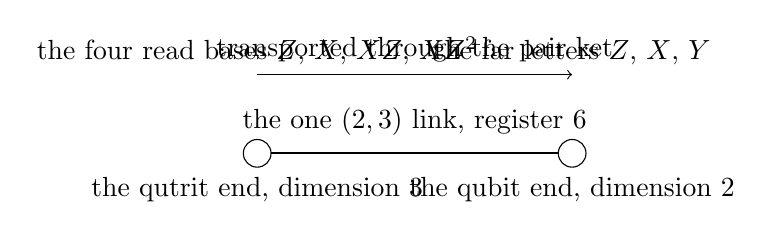
\begin{tikzpicture}[scale=1]
\draw[thick] (0,0) -- (4,0);
\filldraw[fill=white] (0,0) circle (5pt) node[below=5pt] {the qutrit end, dimension 3};
\filldraw[fill=white] (4,0) circle (5pt) node[below=5pt] {the qubit end, dimension 2};
\node at (2,0) [above=3pt] {the one $(2,3)$ link, register $6$};
\node at (0,1) [above] {the four read bases $Z$, $X$, $XZ$, $XZ^{2}$};
\node at (4,1) [above] {the far letters $Z$, $X$, $Y$};
\draw[->] (0,1) -- (4,1);
\node at (2,1) [above=1pt] {transported through the pair ket};
\end{tikzpicture}\caption{The one link of the alpha package, its two ends, the four read bases at the qutrit end and the three far letters of the triplet at the qubit end.}\end{figure}
\end{chproof}
\section{The stabilizer of the pair ket and the unbroken charge}\label{mod:V-1-D541778-w-stab}
\begin{chwall}[The stabilizer of the pair ket and the unbroken charge]\label{box:V-1-D541778-w-stab:1}
The unbroken generator of the stabilizer of the pair ket parts from the central generator of the letter at the third level of the qutrit end. The stabilizer of the pair ket inside the identification algebra of the (2,3) link is the subalgebra of dimension four with its center one line at $i\,\mathrm{diag}(1,1,-1,-1,0)$, the pairs of the joint matching group fixing the pair ket 128 and 32 within the determinant bound with their center of order four at the phase powers of that line; the unbroken generator annihilates the pair ket, the scalar zero, while the central generator $i\,\mathrm{diag}(3,3,-2,-2,-2)$ acts on it at the scalar one; its blocks at the center slots of the qutrit end are no scalar, $-1,-1,0$ against $-2$, so it is no functional on the records in the sense of the central functional $3,-2$, parting first at the first slot, the center slot of the qutrit end, and at the third level, zero against minus two, with the decomposition one third of the traceless unit less one third of the second diagonal less two thirds of the third diagonal; the 172 records weighted by the unbroken generator in place of the central functional sum to zero over the register 31104 against the closed form $79 + 48\sqrt{2} + 42\sqrt{3} + 3\sqrt{6}$ over 31104, re-met equal under the central functional; both faces printed, the constant kept at its exact element.
The first face, the unbroken generator equal to the functional at the reads so that the count and the closed form stand and the charge of the letter is at once the central generator and the unbroken generator, reads no, the functional at the slots parting, the scalar on the pair ket parting, zero against one, and the count parting, zero against the closed form; the second face, the unbroken generator parting from the functional at the reads with the first parting slot named with both functionals and the closed form under the unbroken generator a different exact element named, reads yes, the first parting at the center slot of the qutrit end, minus two against $-1,-1,0$, and the count zero over 31104 against the closed form. Open is the charge of the letter: the acting center and the unbroken center of the stabilizer are two different lines of the algebra, the one acting on the pair ket at the scalar one and moving no slot letter, the other leaving the pair ket invariant with its third level at zero, and the closed form stands under the central functional alone.
\end{chwall}
\chstanding{an open result}
\chdeps{Definitions 1.1 to 1.6 and Theorem 124.1}{no theorem beyond it at this release}
The letter selects a charge by centrality, the one central line of the identification algebra of the (2,3) link, which acts on the pair ket as a scalar. One may instead ask for the subgroup that leaves the pair ket invariant and take the center of that subgroup as the unbroken charge. At the (2,3) link the two choices differ. The stabilizer is four dimensional and its center is the line of the generator with entries one, one at the qubit end and minus one, minus one, zero at the qutrit end, which kills the pair ket outright and leaves the third level of the qutrit untouched, whereas the central generator of the letter has the entries three, three and minus two, minus two, minus two and reads one on the pair ket. Weighting the 172 records of the two reads by the unbroken generator gives zero, so the closed form of the count survives only under the central functional. At the homogeneous (2,2) link the two lines coincide, which is why the parting is a property of the third level.
\begin{chbridge}
In a gauge theory the unbroken charge is the generator of the subgroup under which the vacuum is invariant, and in the electroweak theory the electric charge is the one combination of the hypercharge and the third weak isospin component that annihilates the vacuum expectation value \cite{Weinberg1967,Peskin1995}. The correspondence is by name.
\end{chbridge}
\begin{chproof}[finite computation with its exact part]
The premises of this derivation are the axiom and the six definitions of chapter~\ref{mod:FRAMEWORK}, the link and its six genres of chapter~\ref{mod:I-2-link-and-its-six-genres}, a theorem, the records, reads and the Born count of chapter~\ref{mod:I-3-records-reads-and-the-born-count-the-gain-lemma}, a theorem, the gauge group of chapter~\ref{mod:IV-1-gauge-invariance-as-the-known-clause}, a theorem, and the fine-structure constant at the one link of chapter~\ref{mod:V-1-fine-structure-constant-at-the-one-link}, a theorem. The chain of premises runs back to the axiom through those chapters, and the longest such chain in this compendium is twelve chapters long.
\textit{The object.} The one (2,3) link has a qubit end of dimension two and a qutrit end of dimension three, the register of dimension five and the tensor register $\mathbb{C}^{2}\otimes\mathbb{C}^{3}$ of dimension six. The identification algebra of the link has twelve basis elements with the brackets closed at 144 of 144 and the center one line, the traceless unit; it acts on the tensor register by $X_{1}\otimes 1 + 1\otimes X_{2}$, and the pair ket on the common support of dimension two is the six-vector with the entries one at the matched directions $(0,0)$ and $(1,1)$ and zero elsewhere. The figure draws the link with its five levels and the two generators at them.
\textit{The procedure.} Compute the subalgebra annihilating the pair ket under the tensor action, the null space of the action on the twelve coefficients. Take its center. Compare the central generator of that center with the central generator of the letter at three places, the scalar on the pair ket, the blocks at the four slots of the two reads in the slot order center, far, center, far at the end dimensions three, two, three, two, and the entries at the three levels of the qutrit end. At the finite face count the pairs of the joint matching group of order 12288 that fix the pair ket and the order of their center. Weight the 172 records of the two reads, the roster of 169 in the blocks 24, 64, 24, 24, 9 and 24 at the slots eight, three, eight and three and the three commutators, by the scalar of each generator on the pair ket, summing the weights one at 79, root two at 48, root three at 42 and root six at 3 over the register $31104 = 24\cdot 36\cdot 36$.
\textit{The smallest instance.} The null space has rank eight at the twelve coefficients, so the stabilizer has dimension four, with the basis in the coordinates of the algebra the sum of the two antisymmetric elements, the difference of the two symmetric imaginary elements, the difference of the first two diagonals, and the first diagonal plus twice the third diagonal less the traceless unit; its center has dimension one, unique, at
\begin{equation} G = i\,\mathrm{diag}(1,1,-1,-1,0), \qquad C = i\,\mathrm{diag}(3,3,-2,-2,-2), \end{equation}
$C$ the central generator of the letter and $G$ the decomposition $\tfrac{1}{3}\,TU - \tfrac{1}{3}\,h_{23} - \tfrac{2}{3}\,h_{34}$, the integers $-1$, $-2$ and $1$ at the scale three. On the pair ket $\lvert 0,0\rangle + \lvert 1,1\rangle$ the tensor action reads the qubit entry plus the qutrit entry at each matched direction,
\begin{equation} \adjustbox{max width=\dimexpr\linewidth-3em\relax}{$\displaystyle \begin{gathered} C:\ 3 + (-2) = 1 \ \text{at both directions, the scalar } 1; \\ G:\ 1 + (-1) = 0 \ \text{at both directions, the scalar } 0 . \end{gathered}$} \end{equation}
At the four slots the blocks of $C$ are the scalar $-2$ at the two center slots and the scalar $3$ at the two far slots, the central functional $3,-2$, while the blocks of $G$ are $-1,-1,0$ at the center slots, no scalar, and the scalar $1$ at the far slots; the first parting is at the first slot, the center slot of the qutrit end, and at the third level of the qutrit, $0$ against $-2$. At the finite face 128 pairs of the joint matching group fix the pair ket, 32 of them within the determinant bound, equal to the order of the matching group at the qubit end, and their center has order four at the phase powers of the line of $G$. The count of the records weighted by the scalar of each generator is
\begin{equation} \text{under } C:\ \frac{79 + 48\sqrt{2} + 42\sqrt{3} + 3\sqrt{6}}{31104}, \qquad \text{under } G:\ \frac{0}{31104} = 0 , \end{equation}
the first equal to the closed form of the count at the matching cell and the second a different exact element, zero. At the homogeneous (2,2) link, read as a control, the center of the stabilizer is the line $1,1,-1,-1$, equal to the central generator there, with the pair scalar zero, so the two lines coincide where the third level is absent.
\textit{The check.} The counter-tests alter the construction singly and read what moves. Striking the support to the matched directions $(0,0)$ and $(1,2)$ moves the center generator to $1,1,-1,0,-1$, thirteen cells moved. Striking the third level, the qutrit read as a qubit with the (2,2) algebra at seven elements, makes the unbroken generator $1,1,-1,-1$ equal to the central generator as a functional and moves the first parting to the count, thirty-four cells moved. Dropping the determinant bound widens the algebra by the identity at the qutrit end to thirteen elements, the stabilizer to dimension five with a center of dimension two, no one generator, fifty cells moved. Striking the text unmeets the gate. Reading the transpose of the matching map moves the tensor action. Each alteration moves the cells it names. The result was reproduced by an independent route, two engines built apart, the keyed-map and fraction route against the array route, equal at every cell, with the twelve controls the same.
\chcert{172}
\begin{figure}[h]\centering\begin{adjustbox}{max width=\linewidth}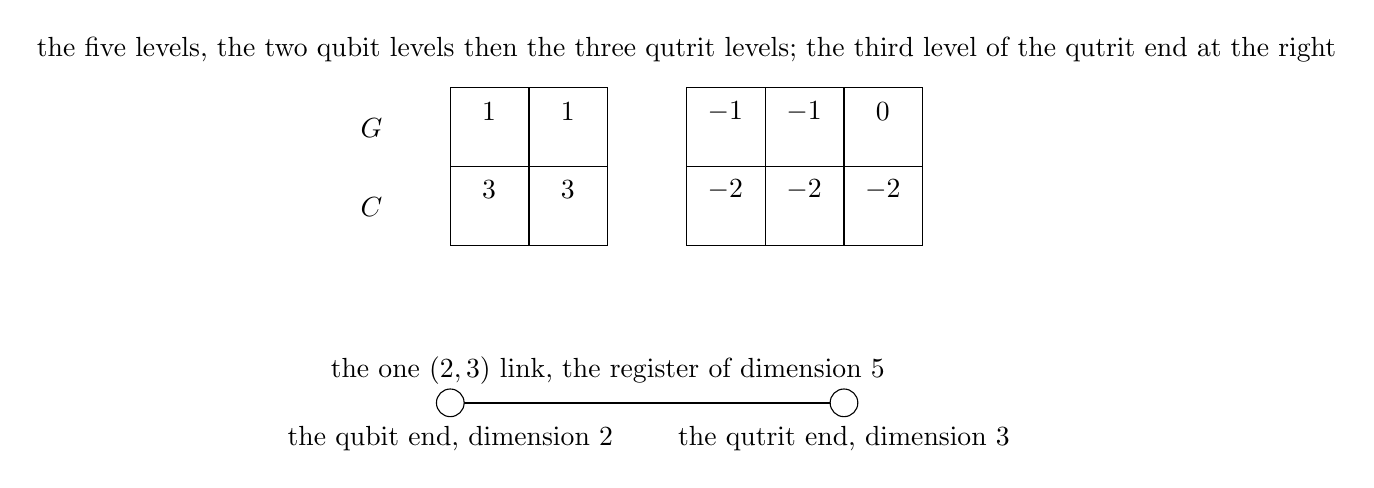
\begin{tikzpicture}[scale=1]
\draw[thick] (0,0) -- (5,0);
\filldraw[fill=white] (0,0) circle (5pt) node[below=5pt] {the qubit end, dimension 2};
\filldraw[fill=white] (5,0) circle (5pt) node[below=5pt] {the qutrit end, dimension 3};
\node at (2,0) [above=3pt] {the one $(2,3)$ link, the register of dimension 5};
\foreach \x/\c/\g in {0/3/1, 1/3/1, 3/-2/-1, 4/-2/-1, 5/-2/0} {\draw (\x,2) rectangle (\x+1,3); \node at (\x,2) [xshift=14pt, yshift=20pt] {$\c$}; \draw (\x,3) rectangle (\x+1,4); \node at (\x,3) [xshift=14pt, yshift=20pt] {$\g$};}
\node at (-1,2) [yshift=14pt] {$C$};
\node at (-1,3) [yshift=14pt] {$G$};
\node at (3,4) [above=6pt] {the five levels, the two qubit levels then the three qutrit levels; the third level of the qutrit end at the right};
\end{tikzpicture}\end{adjustbox}\caption{The one (2,3) link and its register of five levels, with the entries of the central generator $C$ of the letter and of the unbroken generator $G$ of the stabilizer at each level; the two part at the third level of the qutrit end.}\end{figure}
\end{chproof}
\section{The Ward functional and the dressing per unit at the one link}\label{mod:V-1-D541806-w-wdfu}
\begin{chwall}[The Ward functional and the dressing per unit at the one link]\label{box:V-1-D541806-w-wdfu:1}
The dressing equals the dressing per unit of the conserved count at the pair-scalar reading and at the typed-count face at the slots at the sector level, and parts from it at the typed-count face at the record level. The Ward identity of the one (2,3) link holds at the unit functional $1,1,1$ alone among the three functionals the item names, 48 of 48 paths and 172 of 172 records, the central generator sum and the unbroken sum at 0 of 48 and 0 of 172 with the vertices $-24$ and $-8$ against the counts $-12$ and $-4$, the holding functional named from the tables of the Ward result; its scalar on the pair ket is $5/6$, against one at the acting center and zero at the unbroken generator, its typed-count face one at every slot and its per-direction face $1/3$ and $1/2$ at the center and far slots; the dressing $79 + 48\sqrt{2} + 42\sqrt{3} + 3\sqrt{6}$ over 31104 equals the closed form; the dressing per unit is the same element at the pair-scalar reading, the unit $5/6$ at every record, and at the typed-count face at the sector level, the unit two at every record, one read one unit, with the ratio one at both, and $158 + 96\sqrt{2} + 82\sqrt{3} + 3\sqrt{6}$ over 31104 at the typed-count face at the record level, the unit one at the three commutators and the record R169 at no read, with the ratio $129644176/62960159 - (89820/62960159)\sqrt{2} - (2093110/62960159)\sqrt{3} - (1212789/62960159)\sqrt{6}$; the per-direction face beside at a different element at both levels; the first parting record R001 at the per-unit values one, one and two, the two levels parting first at R169; both faces printed, the constant kept at its exact element.
The first face, the ratio one at every reading, the unit of the conserved count one read and the letter dressing already the coupling per unit, reads no, the ratio one at the pair-scalar reading and at the typed-count face at the sector level but a different exact element at the typed-count face at the record level; the second face, the ratio a different exact element at every reading, a factor read off the functional at the reads, reads no, the ratio one at two of the three readings. Open is the reading of the record ends: the two faces of the item are the two faces of the unit of charge, and the record level of the Ward result, the commutators at one read and R169 at none, parts from the sector level of the stabilizer result at those four records alone, the parting that of the record ends at the two parent tables and not of the pair scalar, both readings printed.
\end{chwall}
\chstanding{an open result}
\chdeps{Definitions 1.1 to 1.6 and Theorem 124.1}{no theorem beyond it at this release}
The question is whether the dressing of the one link, the exact element the 172 records of its two reads sum to over the register, is already the dressing per unit of the conserved count, so that the identification at the link is complete with no body. Three functionals are candidates for the conserved count, and the Ward identity, the vertex equal to the count with the line vanishing at every path and every record, holds for the unit functional alone. Reading the unit per record in two ways gives two answers: at the pair-scalar reading every record carries the same unit, five sixths, and at the typed-count face at the sector level every record carries two units, one per read, so in both the dressing per unit is the dressing itself and the ratio is one; but at the record level of the Ward tables the three commutators carry one unit and one record carries none, the per-unit sum becomes a different exact element, and the ratio is the quotient printed in the statement. The result prints both readings and names the first record at which they part.
\begin{chbridge}
The Ward identity of electrodynamics relates the vertex function to the electron propagator and guarantees that the charge renormalization is the same for every charged field, so that the coupling measured per unit of charge is universal, and the dressed coupling at zero momentum transfer is the fine-structure constant \cite{Ward1950,Peskin1995}. The correspondence is by name.
\end{chbridge}
\begin{chproof}[finite computation with its exact part]
The premises of this derivation are the axiom and the six definitions of chapter~\ref{mod:FRAMEWORK}, the records, reads and the Born count of chapter~\ref{mod:I-3-records-reads-and-the-born-count-the-gain-lemma}, a theorem, the gauge group of chapter~\ref{mod:IV-1-gauge-invariance-as-the-known-clause}, a theorem, the fine-structure constant at the one link of chapter~\ref{mod:V-1-fine-structure-constant-at-the-one-link}, a theorem, and the stabilizer of the pair ket of the present chapter, an open result. The chain of premises runs back to the axiom through those chapters, and the longest such chain in this compendium is twelve chapters long.
\textit{The object.} The one (2,3) link is read twice, the ket copy at the slot end of dimension three and the bra copy at the partner end of dimension two, so that a record of the two reads has four slots in the order center, far, center, far at the end dimensions three, two, three, two. The 172 records are the roster of 169 in the blocks 24, 64, 24, 24, 9 and 24 at the slots eight, three, eight and three and the three commutators; their weights by the exchanges are one at 79 records, root two at 48, root three at 42 and root six at 3, the sectors 79, 48, 42 and 3 equal to the slot polynomials in eight and three, over the register $31104 = 24\cdot 36\cdot 36$. The figure draws the two reads with their four slots.
\textit{The procedure.} Re-run the Ward identity at the one link at the eight admitted orderings of one read and three joins, 48 paths at the three inserted dimensions, for each functional of the frozen list of twenty-four and for the unbroken sum beside: the typed count at the polarity plus reads $-1$ at the dimension two, $1$ at the dimension three and $0$ at the dimension four, the vertex is the functional of the typed count plus the link-pair sum, the count is the functional of the typed count, and the line is the functional of the link-pair sum, zero exactly when the per-dimension sums at the two ends agree; the identity holds at a functional when the vertex equals the count at every path and every record. Name the holding functional. Then read its unit at the four slots at the typed-count face, the per-dimension sum, and at the per-direction face, the block scalar; read its scalar on the pair ket under the tensor action on the six-vector; and divide the dressing by the unit per record at each reading to obtain the dressing per unit and its ratio to the dressing.
\textit{The smallest instance.} The identity holds at the unit functional $1,1,1$ alone, the vertex, the count and the line all zero at the polarity plus, 48 of 48 paths and 172 of 172 records; at the per-dimension sum of the central generator $6,-6,0$ the vertex is $-24$ against the count $-12$ with the line $-12$, and at the unbroken sum $2,-2,0$ the vertex is $-8$ against the count $-4$ with the line $-4$, at 0 of 48 paths and 0 of 172 records each. The unit of the holding functional is one at every slot at the typed-count face and, at the per-direction face, $1/3$ at the center slots and $1/2$ at the far slots, four and six at the scale twelve, against $-2$ and $3$ for the central generator; its scalar on the pair ket is
\begin{equation} \tfrac{1}{2} + \tfrac{1}{3} = \tfrac{5}{6}, \end{equation}
ten at the scale twelve, against one at the acting center and zero at the unbroken generator. The dressing is the sum of the weights over the register,
\begin{equation} D = \frac{79 + 48\sqrt{2} + 42\sqrt{3} + 3\sqrt{6}}{31104}, \end{equation}
equal to the closed form of the matching cell. At the pair-scalar reading every record carries the unit $5/6$ and at the typed-count face at the sector level every record carries two units, one per read, so at both the dressing per unit is $D$ and the ratio is one. At the typed-count face at the record level the three commutators carry one unit and the record R169 carries none, so the per-unit sum is
\begin{equation} \adjustbox{max width=\dimexpr\linewidth-3em\relax}{$\displaystyle \begin{gathered} D' = \frac{158 + 96\sqrt{2} + 82\sqrt{3} + 3\sqrt{6}}{31104}, \\ \frac{D'}{D} = \frac{129644176}{62960159} - \frac{89820}{62960159}\sqrt{2} - \frac{2093110}{62960159}\sqrt{3} - \frac{1212789}{62960159}\sqrt{6}, \end{gathered}$} \end{equation}
a different exact element; the first parting record is R001 at the per-unit values one, one and two, and the two levels part first at R169, two against zero, and at the three commutators, two against one. The per-direction face gives a different element at both levels and is printed beside.
\textit{The check.} The counter-tests alter the construction singly and read what moves. Scaling the holding functional by twelve moves the unit at the pair-scalar reading from $5/6$ to ten and every unit with it, the ratio cells unmoved. Putting the central generator sum in place of the holding functional fails the identity at the vertex $-24$ against the count $-12$. Striking the first record leaves 171 records and takes the dressing off the closed form. Reading the transpose of the matching map moves the pair scalar of the unit functional from $5/6$ to $1/6$ and that of the central generator from one to five. Altering the register to the whole register alone moves the dressing. Striking the text unmeets the gate. Each alteration moves the cells it names. The result was reproduced by an independent route, two engines built apart, the keyed-map route against the array route, equal at every cell, with the Ward tables re-met at 144 of 144, 12 of 12 and 72 of 72 cells and the twelve controls the same.
\chcert{172}
\begin{figure}[h]\centering\begin{adjustbox}{max width=\linewidth}\begin{tikzpicture}[scale=1]
\draw[thick] (0,0) -- (4,0);
\filldraw[fill=white] (0,0) circle (5pt) node[below=5pt] {center slot, dimension 3};
\filldraw[fill=white] (4,0) circle (5pt) node[below=5pt] {far slot, dimension 2};
\node at (2,0) [above=3pt] {the ket read of the link};
\draw[thick] (7,0) -- (11,0);
\filldraw[fill=white] (7,0) circle (5pt) node[below=5pt] {center slot, dimension 3};
\filldraw[fill=white] (11,0) circle (5pt) node[below=5pt] {far slot, dimension 2};
\node at (9,0) [above=3pt] {the bra read of the link};
\node at (0,2) [above] {$1$ and $\tfrac{1}{3}$};
\node at (4,2) [above] {$1$ and $\tfrac{1}{2}$};
\node at (7,2) [above] {$1$ and $\tfrac{1}{3}$};
\node at (11,2) [above] {$1$ and $\tfrac{1}{2}$};
\node at (5,3) [above=8pt] {the unit of the holding functional at the four slots, the typed-count face and the per-direction face};
\end{tikzpicture}\end{adjustbox}\caption{The two reads of the one (2,3) link with their four slots in the order center, far, center, far, and the unit of the holding functional at each slot at its two faces.}\end{figure}
\end{chproof}
\section{The alpha Lean derivation, an earlier edition (I)}\label{mod:V-1-D541834-drp9-t1}
\par\noindent\textit{This chapter recorded an earlier edition of the alpha Letter and its Lean check. It is superseded by the Letter and its Lean file in \texttt{papers/alpha} of this repository.}\par
\section{The (2,3) open link against the (2,2) pair ket as the photon}\label{mod:V-1-D541891-rpho-t1}
\begin{chtheorem}[The (2,3) open link against the (2,2) pair ket as the photon]\label{box:V-1-D541891-rpho-t1:1}
The photon of the alpha chain is the (2,3) open link, the one object meeting both criteria, the office zero under the body-alone rule at the reading adopted and the acting central generator at the scalar one, and the (2,2) pair ket at the join is a different object at a different role, the office-zero pairing at the join face without an acting center. The (2,3) open link, one qutrit site read at, one qubit site the far end and one (2,3) link, carries the office zero under the body-alone rule, its one link a dock at a pendant qubit in the dock set and struck, the first power zero, the pair part zero, the dark set empty and the closure zero; the center of the identification algebra at (2,3) is one line at the generator $3,3,-2,-2,-2$ and acts on the pair ket at the scalar one, the central functional $3,-2$. The (2,2) pair ket at the join carries the office zero alike, its one dark link at the act zero, but the center of its algebra annihilates the pair ket, the scalar zero. The objects meeting both criteria number one of two; both faces printed, the constant kept at its exact element.
The first face, one object meeting both criteria, the office zero under the body-alone rule and an acting central generator, the photon one object named and the other a different object with a different role named, reads yes, the (2,3) open link meeting both and the (2,2) pair ket at the join meeting the office criterion alone; the second face, the criteria parting with the office-zero object carrying no acting center and the acting-center object carrying a nonzero office or the rule refusing it, reads no, the office-zero object without an acting center the (2,2) pair ket at the join, the acting-center object with a nonzero office none, the criteria parting at the acting letter alone, the first parting none.
\end{chtheorem}
\chstanding{a theorem}
\chdeps{Definitions 1.1 to 1.6 and Theorem 124.1}{no theorem beyond it at this release}
Two objects of the model have been called the photon. The (2,3) open link of the alpha chain is the object the one-link package reads at, a qutrit read toward a qubit far end; the (2,2) pair ket at the join is the contraction at the join face and the pair of the hub unit. Both carry the office zero under the body-alone rule, since in each the one link is a struck dock, so the office does not tell them apart. The acting center does: the identification algebra at the mixed genre (2,3) has a central line that reads one on the pair ket, while at the homogeneous genre (2,2) the central line reads zero. The one readable genre with an acting center is the (2,3) open link, which is therefore the photon the chain names, and the (2,2) pair ket keeps its own role as the office-zero pairing at the join whose two move classes carry the electromagnetic.
\begin{chbridge}
The photon of electrodynamics is the massless gauge boson of the unbroken U(1), its masslessness tied to the conservation of the electric charge whose generator acts on the charged fields and leaves the vacuum invariant \cite{Peskin1995,Weinberg1995}. The correspondence is by name.
\end{chbridge}
\begin{chproof}[finite computation with its exact part]
The premises of this derivation are the axiom and the six definitions of chapter~\ref{mod:FRAMEWORK}, the link and its six genres of chapter~\ref{mod:I-2-link-and-its-six-genres}, a theorem, the gauge group of chapter~\ref{mod:IV-1-gauge-invariance-as-the-known-clause}, a theorem, the fine-structure constant at the one link of chapter~\ref{mod:V-1-fine-structure-constant-at-the-one-link}, a theorem, and the body-alone office rule of chapter~\ref{mod:VIII-2-body-alone-office-rule}, a theorem. The photon docking at both faces of chapter~\ref{mod:V-8-photon-docking-the-join-face-and-pair-production}, a conditional theorem whose photon word is held by qutrit-qubit pairs, is not among these premises. The chain of premises runs back to the axiom through those chapters, and the longest such chain in this compendium is twelve chapters long.
\textit{The objects.} The (2,3) open link has the sites $t$ of dimension three and $q$ of dimension two and the one link $tq$ of measure six, the slot the end read at and $q$ the far end, the object the one-link package reads at, located at twelve of twelve places, at the package cells, at the abelian-genre result, at the fixed library of webs with its 54 (2,3) link lines and at the forces result among the hub-forming carriers. The (2,2) pair ket at the join has two qubit sites and one (2,2) link of measure four. The figure draws both.
\textit{The procedure.} Read each object as the body-alone rule reads a word at the reading adopted, the measure-struck read with the slot rule, the (3,4)-only dressing, the dark set at the first reading and the link-weight closure: a link that is a dock at a pendant qubit is in the dock set and its act is struck; the first power is the sum of the acts of the unstruck links, the pair part the sum over ordered pairs, the closure the sum over the dark links of the act multiplied by the link law, the office the sum of the three. Then build the identification algebra at each genre from the rules of the package, the antisymmetric, symmetric-imaginary and diagonal elements at the labels of each end and the traceless unit, close the brackets, take the null space of the stacked adjoint brackets as the center, and read its scalar on the pair ket under the tensor action. An object meets both criteria when its office is zero and its center acts, the scalar nonzero.
\textit{The smallest instance.} At the (2,3) open link the one link $tq$ is a struck dock with the act zero, the (2,3) genre lies outside the dark set so the dark set is empty, and
\begin{equation} S_{1} = 0, \qquad P = 0, \qquad C = 0 \ \text{(no dark link)}, \qquad \Omega_{23} = 0 ; \end{equation}
the first power zero equals the first power of the photon read of the pair-ket entry and the chain sum of the package. The identification algebra at (2,3) has twelve basis elements with the brackets closed at 144 of 144 and the center one line, the traceless unit with the diagonal $3,3,-2,-2,-2$, whose tensor action on the pair ket $\lvert 0,0\rangle + \lvert 1,1\rangle$ reads
\begin{equation} 3 + (-2) = 1 \ \text{at both matched directions, the scalar } 1, \end{equation}
acting, the central functional $3,-2$. At the (2,2) pair ket at the join the one link is a struck dock with its one dark link at the act zero, so $\Omega_{22} = 0$ alike, while the central line of the (2,2) algebra, the diagonal $1,1,-1,-1$, reads $1 + (-1) = 0$ on the pair ket, the scalar zero, not acting. So the (2,3) open link meets both criteria and the (2,2) pair ket meets the office criterion alone, one object of two, and the two move classes of the electromagnetic at the forces result, the hub-forming pairing and the (2,2) join across webs, stay with the pair ket at the join at its own role.
\textit{The check.} The counter-tests alter the construction singly and read what moves. Striking the closure moves three cells at the (2,4) free genre and the Higgs word, the two objects holding by construction. Reading the closed (2,3) link in place of the open one, both links unstruck, moves the office to 144 and the face to the second. Reading the (3,3) pair ket in place of the (2,2) moves the office to $\tfrac{6879719125}{84934656} + \tfrac{1675}{21233664}\sqrt{3}$ at the dark (3,3) link and the face to the second. Reading the transpose of the matching map moves the scalars to two and five, both centers acting. Striking the text unmeets the gate. Each alteration moves the cells it names. The result was reproduced by an independent route, two engines built apart, the keyed-map and fraction route against the array route, equal at every cell; the controls read the same at fifteen of sixteen, the sixteenth a comparison mis-keyed at its rule with the cell it compares re-met, disclosed at the entry.
\chcert{12}
\begin{figure}[h]\centering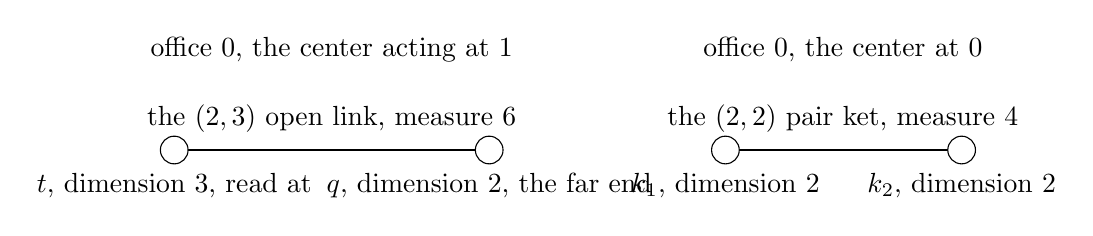
\begin{tikzpicture}[scale=1]
\draw[thick] (0,0) -- (4,0);
\filldraw[fill=white] (0,0) circle (5pt) node[below=5pt] {$t$, dimension 3, read at};
\filldraw[fill=white] (4,0) circle (5pt) node[below=5pt] {$q$, dimension 2, the far end};
\node at (2,0) [above=3pt] {the $(2,3)$ open link, measure $6$};
\node at (2,1) [above] {office $0$, the center acting at $1$};
\draw[thick] (7,0) -- (10,0);
\filldraw[fill=white] (7,0) circle (5pt) node[below=5pt] {$k_1$, dimension 2};
\filldraw[fill=white] (10,0) circle (5pt) node[below=5pt] {$k_2$, dimension 2};
\node at (8,0) [above=3pt, xshift=14pt] {the $(2,2)$ pair ket, measure $4$};
\node at (8,1) [above, xshift=14pt] {office $0$, the center at $0$};
\end{tikzpicture}\caption{The two objects: the (2,3) open link of the alpha chain, which meets both criteria, and the (2,2) pair ket at the join, which meets the office criterion alone.}\end{figure}
\end{chproof}
\begin{figure}[htbp]\centering
\setlength{\unitlength}{1mm}
\begin{picture}(165,42)(0,0)
\put(0,34){\parbox{78mm}{\scriptsize\centering the (2,3) open link: the slot t, the far end q, the one link t-q}}
\put(85,34){\parbox{78mm}{\scriptsize\centering the (2,2) pair ket at the join: the slot k1, the far end k2, the one link k1-k2}}
\put(20,20){\circle{10}}
\put(60,20){\circle{10}}
\put(25,20){\line(1,0){30}}
\put(5,8){\makebox(30,5){\scriptsize t, dimension 3}}
\put(45,8){\makebox(30,5){\scriptsize q, dimension 2}}
\put(105,20){\circle{10}}
\put(145,20){\circle{10}}
\put(110,20){\line(1,0){30}}
\put(90,8){\makebox(30,5){\scriptsize k1, dimension 2}}
\put(130,8){\makebox(30,5){\scriptsize k2, dimension 2}}
\put(20,1){\makebox(40,5){\scriptsize the end read at the slot, passed to the far end}}
\put(105,1){\makebox(40,5){\scriptsize the pairing move at the join face}}
\end{picture}
\par\smallskip
{\scriptsize\setlength{\tabcolsep}{3pt}\begin{adjustbox}{max width=\linewidth}\begin{tabular}{p{52mm}p{52mm}p{52mm}}
 & the (2,3) open link & the (2,2) pair ket at the join \\ \hline
the genre and the sites & (2,3), the sites t, dimension 3 and q, dimension 2 & (2,2), the sites k1, dimension 2 and k2, dimension 2 \\
the office under the body-alone rule at the recorded reading & zero (the first power 0, the closure zero) & zero (the first power 0, the closure zero) \\
the first criterion, the office zero & yes & yes \\
the identification algebra and its centre & 12 basis elements, the centre of dimension 1 at the generator 3, 3, -2, -2, -2 & 7 basis elements, the centre of dimension 1 at the generator 1, 1, -1, -1 \\
the scalar of the centre on the pair ket & 1 & 0 \\
the second criterion, the centre acting & yes & no \\
the stabiliser of the pair ket & of dimension 4 & of dimension 4 \\
meets both criteria & yes & no \\
the role & the recorded object, meeting both criteria & the office-zero pairing at the join face without an acting centre \\
\end{tabular}\end{adjustbox}}
\caption{The recorded photon. Of the two objects the derivation carries, the (2,3) open link of the chain and the (2,2) pair ket at the join, exactly one meets both recorded criteria, the office zero under the body-alone rule at the recorded reading and an acting central generator at the scalar one: the (2,3) open link, read at its slot of dimension three with its far end of dimension two, the recorded object; the (2,2) pair ket at the join has the office zero and no acting centre, a different object at a different role, the objects meeting both 1 of 2 (the photon of the literature is the name for the recorded object).}\label{fig:photon-of-record}
\end{figure}
\section{The (2,3) open link against the (2,2) pair ket, restated}\label{mod:V-1-D541950-rpho-t1}
\begin{chtheorem}[The (2,3) open link against the (2,2) pair ket, restated]\label{box:V-1-D541950-rpho-t1:1}
At its second entry, the photon of the alpha chain is the (2,3) open link, the one object meeting both criteria, the office zero under the body-alone rule at the reading adopted and the acting central generator at the scalar one, and the (2,2) pair ket at the join is a different object at a different role, the office-zero pairing at the join face without an acting center; the cells of the first entry stand unchanged, the (2,3) open link at the office zero with its center acting at the scalar one and the (2,2) pair ket at the office zero with its center at the scalar zero, the objects meeting both criteria one of two, and the control class is re-read holding under the control law, the one comparison mis-keyed at its rule at the first entry re-read at its pinned words so that the controls read the same at sixteen of sixteen; both faces printed, the constant kept at its exact element.
The first face, one object meeting both criteria with the photon one object named and the other a different object with a different role named, reads yes; the second face, the criteria parting with the office-zero object carrying no acting center and the acting-center object carrying a nonzero office or the rule refusing it, reads no, the first parting none.
\end{chtheorem}
\chstanding{a theorem}
\chdeps{Definitions 1.1 to 1.6 and Theorem 124.1}{no theorem beyond it at this release}
The second entry carries the first entry whole and re-reads one thing: the control that compares the office cells of this chapter with the office cells of the pair-ket entry was keyed at the wrong name of one cell at the first entry, so that its comparison read absent against a value that is present and equal. Read at its pinned words the control holds, and with it the whole control class, while no cell of the derivation moves. The photon of the chain remains the (2,3) open link, the object with the office zero and the acting center, and the (2,2) pair ket at the join remains the office-zero pairing without one.
\begin{chbridge}
The photon of electrodynamics is the massless gauge boson of the unbroken U(1), its masslessness tied to the conservation of the electric charge whose generator leaves the vacuum invariant \cite{Peskin1995,Weinberg1995}. The correspondence is by name.
\end{chbridge}
\begin{chproof}[finite computation with its exact part]
The premises of this derivation are the axiom and the six definitions of chapter~\ref{mod:FRAMEWORK}, the fine-structure constant at the one link of chapter~\ref{mod:V-1-fine-structure-constant-at-the-one-link}, a theorem, the body-alone office rule of chapter~\ref{mod:VIII-2-body-alone-office-rule}, a theorem, and the first entry of this result in the present chapter, a theorem. The chain of premises runs back to the axiom through those chapters, and the longest such chain in this compendium is twelve chapters long.
\textit{The procedure.} The procedure is that of the first entry: each object read as the body-alone rule reads a word at the reading adopted, the one link of each a struck dock, and the center of the identification algebra at each genre built from the rules of the package and read on the pair ket under the tensor action; an object meets both criteria when its office is zero and its center acts.
\textit{The smallest instance.} The cells are those of the first entry and are re-met at every one: at the (2,3) open link the first power, the pair part and the closure are zero with the dark set empty,
\begin{equation} \Omega_{23} = 0, \qquad 3 + (-2) = 1 \ \text{the scalar of the center on the pair ket}, \end{equation}
and at the (2,2) pair ket at the join the office is zero with its one dark link at the act zero while the center reads $1 + (-1) = 0$ on the pair ket; the (2,3) open link meets both criteria and the (2,2) pair ket the office criterion alone, one object of two. The figure of the first entry draws both objects.
\textit{The check.} The counter-tests of the first entry stand at their letters: striking the closure, reading the closed (2,3) link in place of the open one, reading the (3,3) pair ket in place of the (2,2), reading the transpose of the matching map and striking the text each move the cells they name, five of five. The one control that read apart at the first entry, the comparison of ten re-run cells of the pair-ket entry with the capture of that entry, was keyed at the first entry to the name of the deciding cell of that entry where its measures table keys it as its first cell, so the comparison read absent against a capture that is present and equal; read at its pinned words the control holds, the nine other cells and the nine word-office cells re-met, and the controls read the same at sixteen of sixteen. The result was reproduced by an independent route, two engines built apart, the keyed-map and fraction route against the array route, equal at every cell.
\chcert{12}
\begin{figure}[h]\centering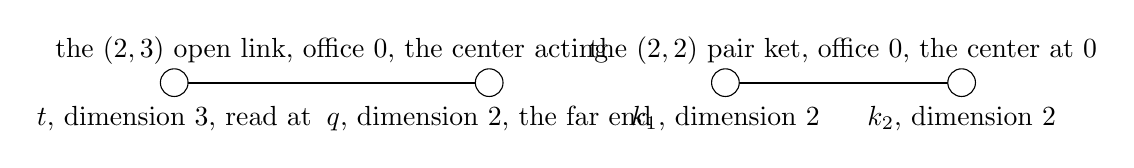
\begin{tikzpicture}[scale=1]
\draw[thick] (0,0) -- (4,0);
\filldraw[fill=white] (0,0) circle (5pt) node[below=5pt] {$t$, dimension 3, read at};
\filldraw[fill=white] (4,0) circle (5pt) node[below=5pt] {$q$, dimension 2, the far end};
\node at (2,0) [above=3pt] {the $(2,3)$ open link, office $0$, the center acting};
\draw[thick] (7,0) -- (10,0);
\filldraw[fill=white] (7,0) circle (5pt) node[below=5pt] {$k_1$, dimension 2};
\filldraw[fill=white] (10,0) circle (5pt) node[below=5pt] {$k_2$, dimension 2};
\node at (8,0) [above=3pt, xshift=14pt] {the $(2,2)$ pair ket, office $0$, the center at $0$};
\end{tikzpicture}\caption{The two objects of the restatement, unchanged from the first statement: the (2,3) open link meeting both criteria and the (2,2) pair ket at the join meeting the office criterion alone.}\end{figure}
\end{chproof}
\section{The alpha Lean derivation, an earlier edition (II)}\label{mod:V-1-D541978-lnat-t1}
\par\noindent\textit{This chapter recorded an earlier edition of the alpha Letter and its Lean check. It is superseded by the Letter and its Lean file in \texttt{papers/alpha} of this repository.}\par
\section{The companion letter, an earlier edition}\label{mod:V-1-D542270-alpha-letter-release-thirty-nine}
\par\noindent\textit{This chapter recorded an earlier edition of the alpha Letter and its Lean check. It is superseded by the Letter and its Lean file in \texttt{papers/alpha} of this repository.}\par
\section{The alpha Lean derivation, an earlier edition (III)}\label{mod:V-1-D542692-ldrf-t1}
\par\noindent\textit{This chapter recorded an earlier edition of the alpha Letter and its Lean check. It is superseded by the Letter and its Lean file in \texttt{papers/alpha} of this repository.}\par
\section{The alpha Lean as a single file, an earlier edition}\label{mod:V-1-D543049-the-alpha-lean-as-a-single-file}
\par\noindent\textit{This chapter recorded an earlier edition of the alpha Letter and its Lean check. It is superseded by the Letter and its Lean file in \texttt{papers/alpha} of this repository.}\par
\section{The re-matching redundancy as the diffeomorphism}\label{mod:V-1-D543680-w-rmdf}
\begin{chwall}[The re-matching redundancy as the diffeomorphism]\label{box:V-1-D543680-w-rmdf:1}
This result is conditional on the entries its provenance names, the open results among them read at their grades, the holonomy entry at its provisional label, the composition riding the lowest grade in its chain. The (2,2) count of the metric is invariant under every re-matching of the re-matching group at every (2,2) link of every established web while the frame moves, and the flux clause of the gauge-group open result stands open at the holonomy entry: at 808 of 808 (2,2) link instances of the ten established webs at the steps zero to three every one of the 1024 joint re-matching pairs carries the pair ket to a vector of the shape (2,2), so the serial count along the run, the whole-web count, the count metric, the register and the tower at the depth read the same figure at every pair and equal the depth-metric and serial-insertion entries at 40 of 40 chain-and-step pairs; the frame, the pair ket $1,0,0,1$ and its transport, moves at 992 of 1024 pairs at every link, first at the electron chain at the step zero; the flux clause as the holonomy entry leaves it is closed at its number conjunct, the determinant exponent equal to the wash integer at 89607 of 89607 fan loops, and open at its element conjunct, the holonomy outside the stabilizer at 66275 of 89607 fan loops, first at a one-link (2,3) loop; the first face unmet at the clause conjunct, the second face named with both cells, the flux-closed reading beside at its own first face.
The first face, the count invariant with the frame moved and the flux clause closed as the holonomy entry leaves it, reads no, the count invariant at every link and the frame moved at the first link but the flux clause open at its element conjunct; the second face, the first link or web where the count moves or the flux clause not closed at the holonomy entry with the count read at that standing, reads yes, the first parting the flux clause at its element conjunct against closed, with the count read at that standing invariant at 808 of 808 links under 1024 pairs per link. Open is the flux clause itself: the holonomy of the transport identity is the swap of the two factors at every odd fan loop and no element of the stabilizer, so the item that places the clause ahead of the invariance does not close.
\end{chwall}
\chstanding{an open result}
\chdeps{Definitions 1.1 to 1.6 and Theorem 124.1}{no theorem beyond it at this release}
A re-matching changes the basis in which the two ends of a link are read, one monomial matrix of fourth-root phases at each end, and the question is whether the metric count, the number of (2,2) links along a chain and the register and tower built from it, is a redundancy of that choice in the way a coordinate change is a redundancy of a geometry. It is: at every (2,2) link of every established web every one of the 1024 pairs of re-matchings carries the pair ket to another vector of the same shape, two by two at Schmidt rank two, so nothing the count reads moves. The frame is not a redundancy: the pair ket and its transport move at all but the thirty-two pairs in which the far matrix is the conjugate of the near one. What the result leaves open is the clause placed ahead of this reading, that the flux of the gauge-group open result closes, which the holonomy entry leaves open at its element conjunct.
\begin{chbridge}
In general relativity a diffeomorphism is a redundancy of the description, the metric transforms as a tensor and every invariant count of the geometry is unchanged, while a frame field is moved by the same transformation, and in a gauge theory the holonomy of a connection around a closed loop measures the flux through it \cite{Wald1984,Peskin1995}. The correspondence is by name.
\end{chbridge}
\begin{chproof}[exhaustive census]
The premises of this derivation are the axiom and the six definitions of chapter~\ref{mod:FRAMEWORK}, the link and its six genres of chapter~\ref{mod:I-2-link-and-its-six-genres}, a theorem, the gauge group of chapter~\ref{mod:IV-1-gauge-invariance-as-the-known-clause}, an open result, the curvature as the graph Laplacian of chapter~\ref{mod:X-1-curvature-as-the-graph-laplacian-washed-over-the-ladder}, a theorem, and the register tower and the metric of chapter~\ref{mod:X-5-register-tower-and-the-metric}, a theorem. The chain of premises runs back to the axiom through those chapters, and the longest such chain in this compendium is twelve chapters long.
By exhaustive enumeration of 827\,392 images, the 808 (2,2) link instances of the ten established webs, the seven established chains and three beside at the steps zero to three, under the 1024 joint pairs of the re-matching group at dimension two, the thirty-two monomial matrices of fourth-root phases at each end, closed at its generators at 96 of 96 and equal to the groups table of the gauge-group entry: the property tested at each image is its shape, the end dimensions read from the image of the pair ket with the Schmidt rank by elimination over the Gaussian rationals at one engine and by matching distinct rows against distinct columns at the other, and beside it whether the pair ket and its transport are moved; the counts by class are the shape (2,2) at every one of the 827\,392 images, the count invariant at 808 of 808 links with the first parting none, the record counts equal to the depth-metric and serial-insertion entries at 40 of 40, and the frame moved at 992 of 1024 pairs at every link with the thirty-two stabilizer pairs fixing it, first at the electron chain at the step zero at its link $a_{1}a_{2}$. The smallest case is that link: with the pair ket $\lvert 00\rangle + \lvert 11\rangle$ and a pair $(U, V)$ of monomial unitaries,
\begin{equation} (U \otimes V)\,(\lvert 00\rangle + \lvert 11\rangle) = (U V^{\mathrm{t}} \otimes 1)\,(\lvert 00\rangle + \lvert 11\rangle), \end{equation}
which has Schmidt rank two since $U V^{\mathrm{t}}$ is invertible, so the shape (2,2) and every count built from it are unchanged, while the vector is fixed only when $U V^{\mathrm{t}}$ is a phase, the thirty-two pairs with $V$ the conjugate of $U$ up to a phase, and moved at the other 992. The flux clause is read as the holonomy entry leaves it, at 89607 fan loops: closed at the number conjunct, the determinant exponent equal to the wash integer at 89607 of 89607, and open at the element conjunct, the holonomy outside the stabilizer at 66275 loops, the odd loops, and inside at 23332, first at a one-link (2,3) loop; the flux-closed reading beside, the clause taken as closed at its number conjunct, meets the first face with the first parting none and is printed beside.
The counter-tests alter the construction singly and read what moves. Striking the re-matching group at the first link to the identity alone moves the first moving link. Reading a (2,3) link in place of the (2,2) re-types it at the joint group of 12288 pairs and moves the invariance to 807 of 808. Holding the frame fixed at the thirty-two stabilizer pairs moves the moved count to zero with the invariance standing. Reading the odd loops alone moves the element conjunct to inside at none of 66275. Striking the text unmeets the gate. Each alteration moves the cells it names, five of five. The result was reproduced by an independent route, two engines built apart, the Gaussian-integer route against the fraction route, equal at every cell, with the fifteen controls the same.
\chcert{827392}
\end{chproof}
\par\medskip\noindent{\itshape The constant read, the next chapter turns to the dipole factor of the electron.}\label{narr:close:5-1}\par
\section{The electron anomalous dipole factor through order three}\label{mod:V-2-electron-anomalous-dipole-factor-through-order-three}
\chdesig{7-2}{5-2}{V-2-electron-anomalous-dipole-factor-through-order-three}{V-2-electron-anomalous-dipole-factor-through-order-three}
\label{narr:open:5-2}Theorem~141.1 gives the electron dipole factor at order three from the self-terms, resting on the records, the probe and the constant of chapter 5-1.
\begin{chconditional}[The electron dipole factor at order three from the self-terms]\label{box:V-2-electron-anomalous-dipole-factor-through-order-three:1}
This result is conditional on the axiom text and on the results of the chapters named as its premises in the derivation below, each at its own standing.
At the anomaly web with the measuring body in place the readout at order two equals the sum of the tabulated self-terms at all eight own-link records, and the order-three term is zero, the direct record sum graded by the surviving exchange count terminating at order three at all eighteen joined webs; the readings beside, the apparatus weight at one part alone, part and are recorded beside the result.
\end{chconditional}
\chstanding{a conditional theorem}
\chdeps{Definitions 1.1 to 1.6, Theorems 18.1 to 18.4 and Open results 18.5 and 18.6, Theorems 28.1 and 28.2, Open results 28.3 and 28.4 and Theorem 28.5 and Theorem 124.1}{Theorem 79.1 and Theorem 143.1}
The anomaly is the sum of the self-terms (the self-energy terms) through the photon: the sum over the thirteen bodies of the construction at the standing reading, the probe electron at the docking face under the depth rule, equals the two-vertex term at order one and not the order-two electron term, the excess at order two carried by the bodies of depth zero entering beside the electron, the up quark through the (2,2) pair at the photon dock and the W word, its twin and the gluon word through their own dark links, with no self-term undefined at any order; a conditional theorem.
One open result stands here. Alpha and the anomaly at the joined web of the electron and the photon at the link-weight placement part at both tests, the readout of the anomaly web against the standing one-link readout among them, the first parting record the pair of the two electron ends, both faces printed.
\begin{chbridge}
The anomalous magnetic dipole factor of the electron, $a_{e} = (g_{e} - 2)/2$, is a power series in $\alpha/\pi$ whose first coefficient is one half \cite{Schwinger1948}, whose second is known in closed form \cite{Petermann1957}, and whose higher coefficients are evaluated through the tenth order \cite{Aoyama2018}; the series is asymptotic and its terms are the sums of the vertex diagrams at each order. The correspondence is by name; the record supplies a web of this theory read at its sinks, a doublet swap sign at the odd cycle, a Dirac form at an established generator and a finite record sum carrying the path-integral name at chapter~\ref{mod:II-1-state-space-from-the-act-outputs}, chapter~\ref{mod:II-5-indistinguishability-and-the-spin-statistics-sign}, chapter~\ref{mod:II-7-path-integral-as-the-finite-record-sum}, chapter~\ref{mod:III-5-spin-and-helicity}, the chapter titled The Dirac equation at the dock (chapter~\ref{mod:V-9-dirac-equation-at-the-dock}, among the instruments), chapter~\ref{mod:VI-2-w-and-the-z-and-their-masses}, chapter~\ref{mod:VI-2b-neutral-lepton-the-hub-unit-with-its-legs-open}, chapter~\ref{mod:VII-5-proton-to-electron-ratio-a-candidate}, chapter~\ref{mod:VIII-1-mass-unit-and-the-first-power}, chapter~\ref{mod:XIV-2-walls-census-in-physics-terms} and chapter~\ref{mod:XIV-7-what-remains-the-ungraded-page}, a step generator at the order coordinate, a first-power operator, a direction functional and an office at the common support carrying the energy, momentum and mass names at chapter~\ref{mod:I-3-records-reads-and-the-born-count-the-gain-lemma}, chapter~\ref{mod:I-6-read-at-a-register-the-probe-and-the-measurement}, chapter~\ref{mod:II-6-energy-and-the-hamiltonian-the-first-power-operator-and-the-step}, chapter~\ref{mod:III-1-order-coordinate-and-its-theorem}, chapter~\ref{mod:III-6-p-c-t-and-cpt}, chapter~\ref{mod:IV-6-conservation-as-the-kernel-of-the-move-matrix}, chapter~\ref{mod:V-7-running-of-the-coupling}, the chapter titled The Dirac equation at the dock (chapter~\ref{mod:V-9-dirac-equation-at-the-dock}, among the instruments), chapter~\ref{mod:VIII-1-mass-unit-and-the-first-power}, chapter~\ref{mod:VIII-5-unified-mass-readout}, chapter~\ref{mod:X-2-field-equation-at-the-counting-face}, the chapter titled The gravitational and cosmological constants table (chapter~\ref{mod:X-9-gravitational-and-cosmological-constants-table}, among the instruments), chapter~\ref{mod:XI-1-second-law-as-the-boundary-count-under-acts} and chapter~\ref{mod:XIV-7-what-remains-the-ungraded-page}, a finite re-matching group at the known clause, a representation census at the open ends and the sinks, an attach-site basis carrying the generation name and a sink class carrying the doublet name at chapter~\ref{mod:IV-1-gauge-invariance-as-the-known-clause}, chapter~\ref{mod:IV-3-representations-from-the-open-end-census}, chapter~\ref{mod:IV-4-cartan-weights-and-the-charge}, chapter~\ref{mod:IV-6-conservation-as-the-kernel-of-the-move-matrix}, chapter~\ref{mod:IV-7-noether-at-the-sinks-and-the-kernel-identification}, chapter~\ref{mod:IV-9-one-rule-of-a-read-and-the-word-table}, chapter~\ref{mod:VI-3-doublets-handedness-and-parity-violation}, chapter~\ref{mod:VII-7-quark-content-and-flavour}, chapter~\ref{mod:VIII-4-three-generations-as-attach-sites} and chapter~\ref{mod:XIV-7-what-remains-the-ungraded-page}, a Higgs attachment at the saturated web, a vacuum expectation row as an office register, a dock share and an office ratio carrying the weak-angle name, sink-basis overlaps carrying the mixing names and a W-word office carrying the Fermi name at chapter~\ref{mod:IV-9-one-rule-of-a-read-and-the-word-table}, chapter~\ref{mod:V-12-koide-class}, chapter~\ref{mod:VI-1-hub-step-as-the-weak-interaction}, chapter~\ref{mod:VI-2-w-and-the-z-and-their-masses}, chapter~\ref{mod:VI-3-doublets-handedness-and-parity-violation}, the chapter titled The charged and neutral currents (chapter~\ref{mod:VI-4-charged-and-neutral-currents}, among the instruments), the chapter titled The Fermi constant and the muon decay (chapter~\ref{mod:VI-5-fermi-constant-and-the-muon-decay}, among the instruments), chapter~\ref{mod:VI-6-weak-angle}, chapter~\ref{mod:VI-7-mixing-the-washed-overlap-and-the-ckm-block}, chapter~\ref{mod:VI-10-higgs-the-closed-hub-read-its-rows-its-mass-and-its-exponent}, chapter~\ref{mod:VIII-1-mass-unit-and-the-first-power}, chapter~\ref{mod:VIII-4-three-generations-as-attach-sites}, chapter~\ref{mod:X-1-curvature-as-the-graph-laplacian-washed-over-the-ladder} and chapter~\ref{mod:XIV-7-what-remains-the-ungraded-page} and a re-matching group with a wash integer, a centralizer weight at the kernel, an enclosed record count carrying the flux name and a counting-face equation carrying the field-equation name at chapter~\ref{mod:I-3-records-reads-and-the-born-count-the-gain-lemma}, chapter~\ref{mod:IV-1-gauge-invariance-as-the-known-clause}, chapter~\ref{mod:IV-4-cartan-weights-and-the-charge}, chapter~\ref{mod:IV-6-conservation-as-the-kernel-of-the-move-matrix}, chapter~\ref{mod:IV-7-noether-at-the-sinks-and-the-kernel-identification}, chapter~\ref{mod:V-1-fine-structure-constant-at-the-one-link}, chapter~\ref{mod:VI-2-w-and-the-z-and-their-masses}, chapter~\ref{mod:X-2-field-equation-at-the-counting-face}, chapter~\ref{mod:X-3-horizon-at-every-rung-and-the-horizon-web-as-a-seeded-saturation}, the chapter titled The gravitational and cosmological constants table (chapter~\ref{mod:X-9-gravitational-and-cosmological-constants-table}, among the instruments), the chapter titled The Chern number (chapter~\ref{mod:XII-4-chern-number}, among the instruments) and chapter~\ref{mod:XIV-7-what-remains-the-ungraded-page}, and the electron, the photon, the quark, the muon, the energy, the flavor, the W, and the gluon correspond there and here by name.
\end{chbridge}
\begin{chproof}[census]
The premises of this derivation are the axiom and the six definitions of chapter~\ref{mod:FRAMEWORK}, the theorem of chapter~\ref{mod:I-3-records-reads-and-the-born-count-the-gain-lemma}, the theorem of chapter~\ref{mod:I-6-read-at-a-register-the-probe-and-the-measurement} and the theorem of chapter~\ref{mod:V-1-fine-structure-constant-at-the-one-link}. The chain of premises runs back to the axiom through those chapters, and the longest such chain in this compendium is twelve chapters long.
The thirteen bodies of the construction are joined at the docking face of the probe electron under the depth rule, the self-term of each body through the photon is read at its order and the sum compared order by order with the two-vertex term and the order-two electron term; the anomaly web is built at the per-web placement with the measuring body in place and the record sum read through order three. The first theorem is conditional on the open results it rests on, among them the binding of hydrogen as the interference term (the cross term) at the two-vertex read; the second rests on the axiom text and the proved results it names alone.
By exhaustive enumeration of the thirteen bodies of the construction joined at the docking face of the probe electron under the depth rule, the self-term of each body through the photon is read at its order and the sum compared order by order with the two-vertex term and the order-two electron term. At the anomaly web with the measuring body in place the readout at order two equals the sum of the self-terms at all eight own-link records and the order-three term is zero at all eighteen joined webs. The smallest case is the anomaly web at the probe reading, the two-dock body of chapter~\ref{mod:II-4-measurement-the-wash-at-one-act-and-the-povm} joined to the photon word, a chain of six sites and five links of type $(2,3)$, by one made link of type $(2,3)$ from the first dock of the body to the last site of the chain, fifteen sites and sixteen links in all, with the two dock links of the body struck and the dressing three at the one hub of the body. From that link list, by the grading of the direct record sum by the surviving exchange count, the order-zero term is the identity, one monomial, the order-one term is the sum over the fourteen unstruck links of the measure multiplied by the dressing (the first power of the web), the order-two term is the pairs, the first power squared, plus the closure of one hundred and five monomials of degree two, and the order-three term is zero, the sum terminating. A reader reproduces the first power from the measures of the five link types, nine, twelve, eight, four and six, the sixty-seven the sum of the measures of the eight unstruck links of the body, the thirty the five chain links and the six the made link,
\begin{equation} \adjustbox{max width=\dimexpr\linewidth-3em\relax}{$\displaystyle \begin{gathered} T_{0} = 1, \qquad T_{1} = 3 \cdot (67 + 30 + 6) = 309, \\ T_{2} = 309^{2} + \text{closure} = 95481 + \text{closure}, \qquad T_{3} = 0, \\ G_{2}(2,2) = \tfrac{5}{216}\,(1 + \sqrt{2}) , \end{gathered}$} \end{equation} the closure part of the order-two term an exact element of the field of the two roots standing at the graded table of this result as a cell, every term an exact element of that field and no digit of any constant displayed here.
The counter-tests alter the objects singly and read what moves, the self-terms struck moving two hundred and forty-nine of the compared keys, the first the order-one term. The five counter-tests stand at their pinned letters, the thirteen controls read the same at both engines and a second engine built apart reproduced every cell.
The machine-checked package named at the reproducibility appendix certifies the statements of this chapter under the definitions of this compendium.
\chcert{13}
\end{chproof}
\par\medskip\noindent{\itshape The muon is next, and its chapter is counted empty.}\label{narr:close:5-2}\par
\section{The instrument tables of this Part}\label{mod:VII-L-the-instrument-tables-at-the-repository}
\chdesig{7-L}{}{VII-L-the-instrument-tables-at-the-repository}{VII-L-the-instrument-tables-at-the-repository}
\begin{chtable}[The instrument tables of this Part]\label{box:VII-L-the-instrument-tables-at-the-repository:1}
This Part lists 3 instrument chapters, printed among the instruments at the end of this compendium as chapters~\ref{mod:V-3-muon-anomalous-dipole-factor} to~\ref{mod:V-9-D538654-w-fcgd}, and the table beneath names each one with its key cells.
\end{chtable}
\chstanding{instrument}
\chdeps{Definitions 1.1 to 1.6}{no theorem beyond it at this release}
The listing moves no cell and states no result of its own. Each instrument stands at the repository as its chapter stood at the previous release of this compendium, and its tables are read there.
\begin{chbridge}
The tables listed here are instruments of the derivation, and no name of the literature is attached at this listing.
\end{chbridge}
\begin{chproof}[instrument]
The listing in full. For each instrument chapter, printed among the instruments at the end of this compendium, the table gives its title, the result boxes it carries, the standing of each box with its citation, and the count of objects its certificate sentence names where it prints one.
{\small
\begin{longtable}{p{38mm}p{63mm}p{30mm}p{14mm}}
\hline
chapter & results & standing & objects \\
\hline
\endhead
The muon anomalous dipole factor & The chapter counted empty & instrument & -- \\
The Dirac equation at the dock & The chapter counted empty & instrument & -- \\
The Dirac equation at the dock & The Dirac form at an established generator commuting with the rest letter & open result & 8 \\
\hline
\end{longtable}
}
The rule that produced it. Every chapter of this Part whose first standing beyond a placeholder reads instrument is printed among the instruments at the end of this compendium with its tables, and its key cells are the titles of its boxes, its standing lines and its certificate count, read from its text as it stood at the previous release.
No derivation stands in this chapter; the tables stand at the repository.
\emph{Check.} Every file listed was re-read at the repository and read the same as its recorded copy, and the listing was re-cut from the files by a second route.
Nothing stands open at this listing. At this release one result of this Part is re-graded at its chapter: the Koide relation at the dock unit (the chapter 7-12), an open result re-posed at a second route.
\end{chproof}
\label{chend:VII-L-the-instrument-tables-at-the-repository}
\section{Hydrogen: the Rydberg ladder and the fine structure}\label{mod:V-4-hydrogen-the-rydberg-ladder-and-the-fine-structure}
\chdesig{7-4}{5-4}{V-4-hydrogen-the-rydberg-ladder-and-the-fine-structure}{V-4-D538525-w-hyjh}
\label{narr:open:5-4}Theorem~143.1 reads hydrogen from the held carrier, with the ladder and the fine structure, and Open result~144.1 states the hyperfine interval as the junction holonomy at the hydrogen sink as an open result.
\begin{chconditional}[Hydrogen from the held carrier]\label{box:V-4-hydrogen-the-rydberg-ladder-and-the-fine-structure:1}
This result is conditional on the axiom text and on the results of the chapters named as its premises in the derivation below, each at its own standing.
Hydrogen is the held carrier: the photon word held at both ends, the qutrit end at the electron dock and the qubit end at the up core of the proton, is a closed read with a mass reading, and its level-one binding through the electron body is an exact element of the field in the electron unit.
\end{chconditional}
\chstanding{a conditional theorem}
\chdeps{Definitions 1.1 to 1.6, Theorems 18.1 to 18.4 and Open results 18.5 and 18.6, Theorems 28.1 and 28.2, Open results 28.3 and 28.4 and Theorem 28.5, Theorem 57.1 and Open result 57.2, Theorem 124.1, Theorem 141.1 and Open results 245.1 and 245.2, Theorem 245.3, Open results 245.4 to 245.8 and Theorem 245.9}{Open result 144.1, Theorem 145.1, Theorem 150.1, Open result 228.1 and Theorem 229.1}
The held pendant pair at rank $n$ is the washed symmetric power of $n$ less one passages along the bond, so the level-$n$ binding is the level-one binding over $n$ squared at every rank from one to eight.
The fine structure is the dark cut of the bond at every one of the eight links of the held chain with the self-join at the vertex at the second order, the two-vertex term multiplied by the square of the cut gain, conditional on the admission of the second-order read at the (2,3) link, a posed step.
The ladder is re-derived from the register rule, the per-record ladder is exact at every rank and no pure power of the rank, and the two-vertex ladder equals one over the rank squared at all eight ranks with no step posed.
The hydrogen body is a probe of the proton: the proton-over-electron mass ratio read off its joined Born reading is an exact rational, the ratio of the two offices, an output compared at the comparison table.
The Lamb shift is a composed cell, every self-term through the photon carried at the second-order register of its type, zero at every rung at the probe read and nonzero at the body alone; the level-one binding is the two-vertex term at the bond, the Rydberg constant in the electron unit the ladder cell of the held carrier; the joined seed of the electron and the proton sink is itself a sink of the saturation at one (2,3) bond; and the Lamb interval at the hydrogen sink, the s self-term less the p self-term at rung two, is one exact element, positive and split.
One open result stands here. The hyperfine interval is not one cell as yet: the definitions admit more than one reading of the dipole read and the orientation, zero at the twirl reading and twice the joined read at the far-face-sign reading, twenty-two distinct cells over sixty readings. A further open result placed here, the mass ratio at the capped hydrogen web, is cited at its own standing.
\begin{chbridge}
The levels of hydrogen fall as the inverse square of the principal quantum number \cite{Bohr1913}, the fine structure splits each shell at the relative order $\alpha^{2}$ \cite{Sommerfeld1916}, the Lamb shift lifts the degeneracy the Dirac equation leaves at the second shell \cite{Lamb1947}, and the hyperfine interval of the ground state is the maser line \cite{Ramsey1990}. The correspondence is by name; the record supplies a web of this theory read at its sinks, a doublet swap sign at the odd cycle, a Dirac form at an established generator and a finite record sum carrying the path-integral name at chapter~\ref{mod:II-1-state-space-from-the-act-outputs}, chapter~\ref{mod:II-5-indistinguishability-and-the-spin-statistics-sign}, chapter~\ref{mod:II-7-path-integral-as-the-finite-record-sum}, chapter~\ref{mod:III-5-spin-and-helicity}, the chapter titled The Dirac equation at the dock (chapter~\ref{mod:V-9-dirac-equation-at-the-dock}, among the instruments), chapter~\ref{mod:VI-2-w-and-the-z-and-their-masses}, chapter~\ref{mod:VI-2b-neutral-lepton-the-hub-unit-with-its-legs-open}, chapter~\ref{mod:VII-5-proton-to-electron-ratio-a-candidate}, chapter~\ref{mod:VIII-1-mass-unit-and-the-first-power}, chapter~\ref{mod:XIV-2-walls-census-in-physics-terms} and chapter~\ref{mod:XIV-7-what-remains-the-ungraded-page}, a dark-genre readability carrying the confinement name, a star office at the common support carrying the nucleon-mass name, a star read at transfer carrying the form-factor name and joined saturations carrying the hadron and nuclear names at chapter~\ref{mod:I-4-moves-in-one-table}, chapter~\ref{mod:III-6-p-c-t-and-cpt}, chapter~\ref{mod:III-7-order-theorem-group-moves-and-transfers}, chapter~\ref{mod:V-1-fine-structure-constant-at-the-one-link}, chapter~\ref{mod:V-7-running-of-the-coupling}, chapter~\ref{mod:V-10-lepton-ladder-as-hub-assemblies}, chapter~\ref{mod:VI-7-mixing-the-washed-overlap-and-the-ckm-block}, chapter~\ref{mod:VII-1-confinement-as-the-dark-genre-readability}, chapter~\ref{mod:VII-3-nucleon-structure-and-the-form-factor}, chapter~\ref{mod:VII-4-proton-as-a-seeded-sink}, chapter~\ref{mod:VII-5-proton-to-electron-ratio-a-candidate}, chapter~\ref{mod:VII-6-hadron-spectrum-and-the-mesons}, chapter~\ref{mod:VII-7-quark-content-and-flavour}, the chapter titled Chiral breaking and the theta angle (chapter~\ref{mod:VII-8-chiral-breaking-and-the-theta-angle}, among the instruments), the chapter titled The mesons and the nucleon at the cap (chapter~\ref{mod:VII-9-mesons-and-the-nucleon-at-the-cap}, among the instruments), chapter~\ref{mod:IX-6-binding-as-the-pairing-records-the-deuteron-and-the-alpha}, chapter~\ref{mod:IX-7-nuclear-rows-at-the-joined-seeded-web}, chapter~\ref{mod:X-7-dark-matter-as-the-dock-free-sinks}, chapter~\ref{mod:XI-4-order-parameter-at-the-stop-condition}, chapter~\ref{mod:XI-5-phase-transition-as-the-sink-class-change} and chapter~\ref{mod:XIV-7-what-remains-the-ungraded-page}, an isometry algebra of the Hermitian split at the Lorentz brackets, a lattice point group, boosts from the order register and a transverse traceless part at the open read, every one a finite or algebraic object of this theory carrying the group name at chapter~\ref{mod:III-2-rotation-group}, chapter~\ref{mod:III-3-lorentz-group-and-the-signature}, chapter~\ref{mod:III-4-boosts-and-the-one-unit}, chapter~\ref{mod:III-5-spin-and-helicity}, the chapter titled Causal structure and general covariance (chapter~\ref{mod:III-8-causal-structure-and-general-covariance}, among the instruments) and chapter~\ref{mod:XIV-7-what-remains-the-ungraded-page} and a re-matching group with a wash integer, a centralizer weight at the kernel, an enclosed record count carrying the flux name and a counting-face equation carrying the field-equation name at chapter~\ref{mod:I-3-records-reads-and-the-born-count-the-gain-lemma}, chapter~\ref{mod:IV-1-gauge-invariance-as-the-known-clause}, chapter~\ref{mod:IV-4-cartan-weights-and-the-charge}, chapter~\ref{mod:IV-6-conservation-as-the-kernel-of-the-move-matrix}, chapter~\ref{mod:IV-7-noether-at-the-sinks-and-the-kernel-identification}, chapter~\ref{mod:V-1-fine-structure-constant-at-the-one-link}, chapter~\ref{mod:VI-2-w-and-the-z-and-their-masses}, chapter~\ref{mod:X-2-field-equation-at-the-counting-face}, chapter~\ref{mod:X-3-horizon-at-every-rung-and-the-horizon-web-as-a-seeded-saturation}, the chapter titled The gravitational and cosmological constants table (chapter~\ref{mod:X-9-gravitational-and-cosmological-constants-table}, among the instruments), the chapter titled The Chern number (chapter~\ref{mod:XII-4-chern-number}, among the instruments) and chapter~\ref{mod:XIV-7-what-remains-the-ungraded-page}, and the photon, the electron, the proton, the mass, and the carrier correspond there and here by name.
\end{chbridge}
\begin{chproof}[exact part and census part]
The premises of this derivation are the axiom and the six definitions of chapter~\ref{mod:FRAMEWORK}, the theorem of chapter~\ref{mod:I-3-records-reads-and-the-born-count-the-gain-lemma}, the theorem of chapter~\ref{mod:I-5-saturation-in-one-figure-seeds-waves-termination-sinks}, the theorem of chapter~\ref{mod:I-6-read-at-a-register-the-probe-and-the-measurement}, the open result of chapter~\ref{mod:III-5-spin-and-helicity}, the theorem of chapter~\ref{mod:V-1-fine-structure-constant-at-the-one-link} and the theorem of chapter~\ref{mod:V-2-electron-anomalous-dipole-factor-through-order-three}. The chain of premises runs back to the axiom through those chapters, and the longest such chain in this compendium is twelve chapters long.
The photon word is docked at both ends; the held pendant pair is built at every rank as a symmetric power; the dark cut of the bond is taken at the eight links; the joined Born reading of the hydrogen body is inverted through the first-power composition; the self-terms are carried at the second-order register and composed at every rung; and the joined seed is saturated to its sink, each theorem conditional on the open results it rests on, among them the nucleon reading composition and the admissibility of a dark-link cut.
\textit{The exact part.}
From the photon word, a chain of six sites and five links every one of the qutrit-qubit type, by the docking act (the distilling pair, one link made at each end and one contraction at one link), we obtain the held carrier, its qutrit end docked at the electron dock and its qubit end at the up core of the proton, a closed read with a mass face, the mass face of the held chain thirty-six and the exchanged mass face six root six.
\begin{equation}
\text{the held chain: } 6 \ \text{sites}, \ 5 \ \text{links of type } (2,3); \qquad M_{L} = 36, \qquad M_{\mathrm{exch}} = 6\sqrt{6} .
\end{equation}
From the mass face of the held chain, by the read through the electron body at its dock port $B$-$w_{1}$ (the mass face multiplied by the unit over the register of the body at that face), we obtain the level-one binding in the electron unit as an exact rational at both closure faces, the whole face with the hub unit two hundred and one over the body register two to the thirtieth multiplied by three to the eighteenth, and the cut face with the dock unit sixty-seven over the body register two to the thirty-first multiplied by three to the seventeenth (the port at its cut twenty-four), the two registers cells of the read tables of this result printed in their prime factorizations, both faces printed, and the port-register readings beside, the mass face multiplied by sixty-seven over the port registers thirty-six and twenty-four,
\begin{equation} \adjustbox{max width=\dimexpr\linewidth-3em\relax}{$\displaystyle \begin{gathered} E_{1}^{\mathrm{whole}} = 36 \cdot \frac{201}{2^{30}\cdot 3^{18}} = \frac{67}{2^{28}\cdot 3^{15}}, \\ E_{1}^{\mathrm{cut}} = 36 \cdot \frac{67}{2^{31}\cdot 3^{17}} = \frac{67}{2^{29}\cdot 3^{15}}, \qquad 36 \cdot \tfrac{67}{36} = 67, \\ 36 \cdot \tfrac{67}{24} = \tfrac{201}{2} . \end{gathered}$} \end{equation}
From the held pendant pair at rank $n$, by the washed symmetric power of $n$ less one passages along the bond, we obtain the level-$n$ binding as the level-one binding over $n$ squared at every rank from one to eight, the register of the ladder equal to the dimension of the register of the pair.
\begin{equation}
E_{n} = \frac{E_{1}}{n^{2}}, \qquad n = 1, \dots, 8 .
\end{equation}
\textit{The census part.}
By exhaustive enumeration of the eight ranks of the held chain and of the eight links of the bond, the ladder is built at every rank as a symmetric power and re-met at the register rule, exact at every rank and a pure power of the rank at none, the two-vertex ladder equal to one over the rank squared at all eight ranks with no step posed. The dark cut of the bond is taken at every one of the eight links with the self-join at the vertex at the second order, the two-vertex term multiplied by the square of the cut gain. The joined Born reading of the hydrogen body is inverted through the first-power composition, and the self-terms are carried at the second-order register and composed at every rung. The smallest case, the held chain and its level-one binding, is worked above.
The counter-tests alter the objects singly and read what moves. Docking at one end alone moves the hold cell from a theorem to none with the mass face undefined. The five counter-tests stand at their pinned letters and the thirteen controls read the same at both engines, among them the construction, the figures and the register rule. The result was reproduced by a second engine built apart from the first, the two runs equal at every key. The two body registers of the level-one binding are cells of the read tables of this result, printed in their prime factorizations and re-derived on the page not; the binding itself follows from them by one multiplication.
The machine-checked package named at the reproducibility appendix certifies the statements of this chapter under the definitions of this compendium.
\chcert{8}
\end{chproof}
\begin{figure}[h]\centering
\setlength{\unitlength}{1pt}
\begin{picture}(260,150)
\qbezier(122.2,123.5)(107.1,114.8)(91.9,106.0)
\put(111.1,107.8){\makebox(0,0){\scriptsize $(2,3)$}}
\qbezier(84.1,92.5)(84.1,75.0)(84.1,57.5)
\put(92.1,75.0){\makebox(0,0){\scriptsize $(2,3)$}}
\qbezier(91.9,44.0)(107.1,35.3)(122.2,26.5)
\put(111.1,42.2){\makebox(0,0){\scriptsize $(2,3)$}}
\qbezier(137.8,26.5)(152.9,35.2)(168.1,44.0)
\put(148.9,42.2){\makebox(0,0){\scriptsize $(2,3)$}}
\qbezier(175.9,57.5)(175.9,75.0)(175.9,92.5)
\put(167.9,75.0){\makebox(0,0){\scriptsize $(2,3)$}}
\put(130.0,128.0){\circle{14}}
\put(130.0,128.0){\makebox(0,0){\footnotesize $2$}}
\put(130.0,138.0){\makebox(0,0)[b]{\scriptsize $s_1$}}
\put(84.1,101.5){\circle{14}}
\put(84.1,101.5){\makebox(0,0){\footnotesize $3$}}
\put(84.1,111.5){\makebox(0,0)[b]{\scriptsize $s_2$}}
\put(84.1,48.5){\circle{14}}
\put(84.1,48.5){\makebox(0,0){\footnotesize $2$}}
\put(84.1,58.5){\makebox(0,0)[b]{\scriptsize $s_3$}}
\put(130.0,22.0){\circle{14}}
\put(130.0,22.0){\makebox(0,0){\footnotesize $3$}}
\put(130.0,32.0){\makebox(0,0)[b]{\scriptsize $s_4$}}
\put(175.9,48.5){\circle{14}}
\put(175.9,48.5){\makebox(0,0){\footnotesize $2$}}
\put(175.9,58.5){\makebox(0,0)[b]{\scriptsize $s_5$}}
\put(175.9,101.5){\circle{14}}
\put(175.9,101.5){\makebox(0,0){\footnotesize $3$}}
\put(175.9,111.5){\makebox(0,0)[b]{\scriptsize $s_6$}}
\end{picture}
\caption{The photon word, a chain of six sites and five qutrit-qubit links, each site labeled by its dimension. Held at both ends (the qutrit end at the electron dock, the qubit end at the up core of the proton) it is the hydrogen bond of this chapter.}
\end{figure}
\section{The hyperfine interval as the junction holonomy of hydrogen}\label{mod:V-4-D538525-w-hyjh}
\begin{chwall}[The hyperfine interval as the junction holonomy at the hydrogen sink]\label{box:V-4-D538525-w-hyjh:1}
At the standing hydrogen sink, the electron of the construction and the proton sink joined at the shared dock qubit with the one (2,3) bond between the shared qubit and the proton dock qutrit, the twenty bound walks through the bond and the junction carry the identity on the qubit register at all sixty holonomies at the standing transport, the two orientations equal and the interval between the two reads the zero element; at the ray-cycle reading the junction triangles carry fixed elements at the two orientations, but read through the bond the chains vanish at 54 of the 216 ray triples and the element is undefined at six of the eight triangles; so the junction holonomy read by the bound electron is trivial at the standing transport and undefined at the ray-cycle reading, the hyperfine interval is no output of it as yet, and the fine-structure condition stands undischarged at the junction.
Open is the result, the hyperfine interval an output of nothing as yet; the hydrogen ladder and the fine structure stand at the opening of this chapter and the Lamb shift at chapter~\ref{mod:V-5-lamb-shift-and-the-casimir-effect}.
\end{chwall}
\chstanding{an open result}
\chdeps{Definitions 1.1 to 1.6, Theorem 143.1 and Theorems 235.1 to 235.4 and Open result 235.5}{no theorem beyond it at this release}
\begin{chbridge}
The hyperfine splitting of the ground state of hydrogen is the interval between the two states of the coupled electron and proton spins, proportional to the product of the two magnetic dipole factors and to the electron density at the proton, the transition between them the line of the hydrogen maser \cite{Fermi1930,Ramsey1965}; no value of the interval is displayed at this chapter. The correspondence is by name; the record supplies a web of this theory read at its sinks, a doublet swap sign at the odd cycle, a Dirac form at an established generator and a finite record sum carrying the path-integral name at chapter~\ref{mod:II-1-state-space-from-the-act-outputs}, chapter~\ref{mod:II-5-indistinguishability-and-the-spin-statistics-sign}, chapter~\ref{mod:II-7-path-integral-as-the-finite-record-sum}, chapter~\ref{mod:III-5-spin-and-helicity}, the chapter titled The Dirac equation at the dock (chapter~\ref{mod:V-9-dirac-equation-at-the-dock}, among the instruments), chapter~\ref{mod:VI-2-w-and-the-z-and-their-masses}, chapter~\ref{mod:VI-2b-neutral-lepton-the-hub-unit-with-its-legs-open}, chapter~\ref{mod:VII-5-proton-to-electron-ratio-a-candidate}, chapter~\ref{mod:VIII-1-mass-unit-and-the-first-power}, chapter~\ref{mod:XIV-2-walls-census-in-physics-terms} and chapter~\ref{mod:XIV-7-what-remains-the-ungraded-page}, a dark-genre readability carrying the confinement name, a star office at the common support carrying the nucleon-mass name, a star read at transfer carrying the form-factor name and joined saturations carrying the hadron and nuclear names at chapter~\ref{mod:I-4-moves-in-one-table}, chapter~\ref{mod:III-6-p-c-t-and-cpt}, chapter~\ref{mod:III-7-order-theorem-group-moves-and-transfers}, chapter~\ref{mod:V-1-fine-structure-constant-at-the-one-link}, chapter~\ref{mod:V-7-running-of-the-coupling}, chapter~\ref{mod:V-10-lepton-ladder-as-hub-assemblies}, chapter~\ref{mod:VI-7-mixing-the-washed-overlap-and-the-ckm-block}, chapter~\ref{mod:VII-1-confinement-as-the-dark-genre-readability}, chapter~\ref{mod:VII-3-nucleon-structure-and-the-form-factor}, chapter~\ref{mod:VII-4-proton-as-a-seeded-sink}, chapter~\ref{mod:VII-5-proton-to-electron-ratio-a-candidate}, chapter~\ref{mod:VII-6-hadron-spectrum-and-the-mesons}, chapter~\ref{mod:VII-7-quark-content-and-flavour}, the chapter titled Chiral breaking and the theta angle (chapter~\ref{mod:VII-8-chiral-breaking-and-the-theta-angle}, among the instruments), the chapter titled The mesons and the nucleon at the cap (chapter~\ref{mod:VII-9-mesons-and-the-nucleon-at-the-cap}, among the instruments), chapter~\ref{mod:IX-6-binding-as-the-pairing-records-the-deuteron-and-the-alpha}, chapter~\ref{mod:IX-7-nuclear-rows-at-the-joined-seeded-web}, chapter~\ref{mod:X-7-dark-matter-as-the-dock-free-sinks}, chapter~\ref{mod:XI-4-order-parameter-at-the-stop-condition}, chapter~\ref{mod:XI-5-phase-transition-as-the-sink-class-change} and chapter~\ref{mod:XIV-7-what-remains-the-ungraded-page} and reflections of the Weyl basis at the cap carrying the P, C and T names, a pair symmetry carrying the CPT name and a junction holonomy carrying the theta name at chapter~\ref{mod:I-2-link-and-its-six-genres}, chapter~\ref{mod:III-6-p-c-t-and-cpt}, chapter~\ref{mod:V-1-fine-structure-constant-at-the-one-link}, chapter~\ref{mod:VI-2-w-and-the-z-and-their-masses} and chapter~\ref{mod:XIV-7-what-remains-the-ungraded-page}, and the electron, the proton, and the discrete symmetries correspond there and here by name.
\end{chbridge}
\begin{chproof}[finite computation]
The premises of this derivation are the axiom and the six definitions of chapter~\ref{mod:FRAMEWORK}, the theorem of chapter~\ref{mod:V-4-hydrogen-the-rydberg-ladder-and-the-fine-structure} and the theorem of chapter~\ref{mod:XIII-6-holonomy-and-the-record-transport}. The chain of premises runs back to the axiom through those chapters, and the longest such chain in this compendium is twelve chapters long.
The standing hydrogen sink is built from the electron of the construction and the standing proton sink at the shared dock qubit, the twenty bound walks through the bond and the junction are enumerated, their holonomies are computed at the standing transport at both orientations and the interval between the two reads taken, the junction triangles are read at the ray-cycle reading with the chains through the bond, and the second read, the walk composed twice, is checked unmoved; the result is an open result, the interval zero a parity statement at the bipartite proton sub-web and the undefined elements forced by the (2,3) support.
The procedure. Build the standing hydrogen sink from the electron of the construction and the standing proton sink joined at the shared dock qubit, with the one qutrit-qubit bond between the shared qubit and the proton dock qutrit. Enumerate the twenty bound walks through the bond and the junction. Compute the holonomy of each walk at the standing transport at both orientations as an exact element of the ring of the twenty-fourth root of unity on the qubit register, and take the interval between the two bound reads. Read the junction triangles at the ray-cycle reading with the chains through the bond, and check the second read, the walk composed twice, for movement. The smallest instance is the first reading, the twenty bound walks carry sixty holonomies, every one the identity on the qubit register, so the interval between the two reads is the zero element at all sixty and the two orientations are equal at every walk. At the second reading the junction triangles carry fixed elements at the two orientations, four at the eighteenth power and four at the sixth power of the root, with the second read unmoved,
\begin{equation} \adjustbox{max width=\dimexpr\linewidth-3em\relax}{$\displaystyle \begin{gathered} \#\{\text{bound walks}\} = 20, \qquad \#\{\text{holonomies}\} = 60, \\ H_{w} = z^{0} = 1 \ \text{at all } 60, \qquad \Delta_{\mathrm{hf}} = 0 ; \\ \text{triangles: } z^{18} \cdot 4,\ z^{6} \cdot 4 , \end{gathered}$} \end{equation} so the junction holonomy read by the bound electron is trivial at the standing transport and the hyperfine interval is an output of nothing as yet, which names the parting of this open result. The fine-structure condition at the second read is not discharged at the junction.
The counter-tests alter the objects singly and read what moves. The first moves three cells, the junction cell from yes to no, the capped count and the register. The four counter-tests stand at their pinned letters and the sixteen controls read the same at both engines, the tables consumed unaltered. The result was reproduced by a second engine built apart from the first, the two runs equal at every cell.
\chcert{20}
\end{chproof}
\par\medskip\noindent{\itshape Two effects at the edge of the atom follow in the next chapter.}\label{narr:close:5-4}\par
\section{The Lamb shift and the Casimir effect}\label{mod:V-5-lamb-shift-and-the-casimir-effect}
\chdesig{7-5}{5-5}{V-5-lamb-shift-and-the-casimir-effect}{V-5-lamb-shift-and-the-casimir-effect}
\label{narr:open:5-5}Theorem~145.1 reads the Casimir effect as the boundary count between two sinks, a theorem resting on the records, the saturation and the hydrogen chapter.
\begin{chtheorem}[The Casimir effect as the boundary count between two sinks]\label{box:V-5-lamb-shift-and-the-casimir-effect:1}
The excluded count between two sinks of the saturation placed along a chain of the construction is a definite function of the separation at every separation the chain admits, with one sign, so the Casimir effect is a composed cell of the second-law and chain results: at the standing readings, the chain, the web between and the count face, the excluded records are defined at all forty-four chains and the nonzero differences carry one sign at every one.
\end{chtheorem}
\chstanding{a theorem}
\chdeps{Definitions 1.1 to 1.6, Theorems 18.1 to 18.4 and Open results 18.5 and 18.6, Theorem 143.1 and Open results 245.1 and 245.2, Theorem 245.3, Open results 245.4 to 245.8 and Theorem 245.9}{no theorem beyond it at this release}
The Lamb shift of the theory stands at the hydrogen chapter, at the probe web and at the hydrogen sink, stated there in full and cited here alone.
\begin{chbridge}
The Casimir effect is the attraction of two parallel conducting plates in vacuum, a force per unit area falling as the inverse fourth power of their separation, read as the difference of the zero-point energy of the electromagnetic modes between the plates from that of free space \cite{Casimir1948}; the Lamb shift is the splitting of the two hydrogen levels the Dirac equation leaves degenerate, measured by microwave resonance \cite{Lamb1947} and accounted for by the radiative corrections of quantum electrodynamics at the bound electron \cite{Bethe1947}. The correspondence is by name; the record supplies a Higgs attachment at the saturated web, a vacuum expectation row as an office register, a dock share and an office ratio carrying the weak-angle name, sink-basis overlaps carrying the mixing names and a W-word office carrying the Fermi name at chapter~\ref{mod:IV-9-one-rule-of-a-read-and-the-word-table}, chapter~\ref{mod:V-12-koide-class}, chapter~\ref{mod:VI-1-hub-step-as-the-weak-interaction}, chapter~\ref{mod:VI-2-w-and-the-z-and-their-masses}, chapter~\ref{mod:VI-3-doublets-handedness-and-parity-violation}, the chapter titled The charged and neutral currents (chapter~\ref{mod:VI-4-charged-and-neutral-currents}, among the instruments), the chapter titled The Fermi constant and the muon decay (chapter~\ref{mod:VI-5-fermi-constant-and-the-muon-decay}, among the instruments), chapter~\ref{mod:VI-6-weak-angle}, chapter~\ref{mod:VI-7-mixing-the-washed-overlap-and-the-ckm-block}, chapter~\ref{mod:VI-10-higgs-the-closed-hub-read-its-rows-its-mass-and-its-exponent}, chapter~\ref{mod:VIII-1-mass-unit-and-the-first-power}, chapter~\ref{mod:VIII-4-three-generations-as-attach-sites}, chapter~\ref{mod:X-1-curvature-as-the-graph-laplacian-washed-over-the-ladder} and chapter~\ref{mod:XIV-7-what-remains-the-ungraded-page}, a step generator at the order coordinate, a first-power operator, a direction functional and an office at the common support carrying the energy, momentum and mass names at chapter~\ref{mod:I-3-records-reads-and-the-born-count-the-gain-lemma}, chapter~\ref{mod:I-6-read-at-a-register-the-probe-and-the-measurement}, chapter~\ref{mod:II-6-energy-and-the-hamiltonian-the-first-power-operator-and-the-step}, chapter~\ref{mod:III-1-order-coordinate-and-its-theorem}, chapter~\ref{mod:III-6-p-c-t-and-cpt}, chapter~\ref{mod:IV-6-conservation-as-the-kernel-of-the-move-matrix}, chapter~\ref{mod:V-7-running-of-the-coupling}, the chapter titled The Dirac equation at the dock (chapter~\ref{mod:V-9-dirac-equation-at-the-dock}, among the instruments), chapter~\ref{mod:VIII-1-mass-unit-and-the-first-power}, chapter~\ref{mod:VIII-5-unified-mass-readout}, chapter~\ref{mod:X-2-field-equation-at-the-counting-face}, the chapter titled The gravitational and cosmological constants table (chapter~\ref{mod:X-9-gravitational-and-cosmological-constants-table}, among the instruments), chapter~\ref{mod:XI-1-second-law-as-the-boundary-count-under-acts} and chapter~\ref{mod:XIV-7-what-remains-the-ungraded-page}, a web of this theory read at its sinks, a doublet swap sign at the odd cycle, a Dirac form at an established generator and a finite record sum carrying the path-integral name at chapter~\ref{mod:II-1-state-space-from-the-act-outputs}, chapter~\ref{mod:II-5-indistinguishability-and-the-spin-statistics-sign}, chapter~\ref{mod:II-7-path-integral-as-the-finite-record-sum}, chapter~\ref{mod:III-5-spin-and-helicity}, the chapter titled The Dirac equation at the dock (chapter~\ref{mod:V-9-dirac-equation-at-the-dock}, among the instruments), chapter~\ref{mod:VI-2-w-and-the-z-and-their-masses}, chapter~\ref{mod:VI-2b-neutral-lepton-the-hub-unit-with-its-legs-open}, chapter~\ref{mod:VII-5-proton-to-electron-ratio-a-candidate}, chapter~\ref{mod:VIII-1-mass-unit-and-the-first-power}, chapter~\ref{mod:XIV-2-walls-census-in-physics-terms} and chapter~\ref{mod:XIV-7-what-remains-the-ungraded-page}, a re-matching group with a wash integer, a centralizer weight at the kernel, an enclosed record count carrying the flux name and a counting-face equation carrying the field-equation name at chapter~\ref{mod:I-3-records-reads-and-the-born-count-the-gain-lemma}, chapter~\ref{mod:IV-1-gauge-invariance-as-the-known-clause}, chapter~\ref{mod:IV-4-cartan-weights-and-the-charge}, chapter~\ref{mod:IV-6-conservation-as-the-kernel-of-the-move-matrix}, chapter~\ref{mod:IV-7-noether-at-the-sinks-and-the-kernel-identification}, chapter~\ref{mod:V-1-fine-structure-constant-at-the-one-link}, chapter~\ref{mod:VI-2-w-and-the-z-and-their-masses}, chapter~\ref{mod:X-2-field-equation-at-the-counting-face}, chapter~\ref{mod:X-3-horizon-at-every-rung-and-the-horizon-web-as-a-seeded-saturation}, the chapter titled The gravitational and cosmological constants table (chapter~\ref{mod:X-9-gravitational-and-cosmological-constants-table}, among the instruments), the chapter titled The Chern number (chapter~\ref{mod:XII-4-chern-number}, among the instruments) and chapter~\ref{mod:XIV-7-what-remains-the-ungraded-page}, a table of entries at their grades carrying the Standard Model names, a representation census and a kernel of conserved counts at chapter~\ref{mod:FRAMEWORK}, chapter~\ref{mod:I-5-saturation-in-one-figure-seeds-waves-termination-sinks}, chapter~\ref{mod:III-5-spin-and-helicity}, the chapter titled The standard-model table: the seventy-five entries with their status (chapter~\ref{mod:IV-10-sm-table-the-75-entries-with-their-status}, among the instruments), chapter~\ref{mod:VI-7-mixing-the-washed-overlap-and-the-ckm-block}, chapter~\ref{mod:IX-6-binding-as-the-pairing-records-the-deuteron-and-the-alpha}, the chapter titled The results table re-tallied (chapter~\ref{mod:XVI-1-the-results-table-re-tallied-at-the-cut}) and chapter~\ref{mod:XIV-7-what-remains-the-ungraded-page}, and a twirl fixed point at a cap, a boundary count under acts, a density standings with a limiting ratio and a sink class carrying the order-parameter and phase-transition names at chapter~\ref{mod:I-6-read-at-a-register-the-probe-and-the-measurement}, chapter~\ref{mod:II-1-state-space-from-the-act-outputs}, chapter~\ref{mod:III-7-order-theorem-group-moves-and-transfers}, chapter~\ref{mod:V-7-running-of-the-coupling}, chapter~\ref{mod:VII-4-proton-as-a-seeded-sink}, chapter~\ref{mod:VIII-5-unified-mass-readout}, chapter~\ref{mod:XI-1-second-law-as-the-boundary-count-under-acts}, chapter~\ref{mod:XI-2-thermal-state}, chapter~\ref{mod:XI-3-ensembles-as-cap-readings}, chapter~\ref{mod:XI-4-order-parameter-at-the-stop-condition}, chapter~\ref{mod:XI-5-phase-transition-as-the-sink-class-change}, the chapter titled The equilibrium theorem (chapter~\ref{mod:XI-6-equilibrium-theorem}, among the instruments), chapter~\ref{mod:XI-7-thermodynamic-remainder-and-the-arrow} and chapter~\ref{mod:XIV-7-what-remains-the-ungraded-page}, and the ground state, the energy, the spinor field, the electron, the field equation, the renormalized field theory, and the thermodynamic structure correspond there and here by name.
\end{chbridge}
\begin{chproof}[exact part, finite part and census part]
The premises of this derivation are the axiom and the six definitions of chapter~\ref{mod:FRAMEWORK}, the theorem of chapter~\ref{mod:I-3-records-reads-and-the-born-count-the-gain-lemma}, the theorem of chapter~\ref{mod:I-5-saturation-in-one-figure-seeds-waves-termination-sinks} and the theorem of chapter~\ref{mod:V-4-hydrogen-the-rydberg-ladder-and-the-fine-structure}. The chain of premises runs back to the axiom through those chapters, and the longest such chain in this compendium is twelve chapters long.
Two sinks of the saturation placed at a separation along a chain of the construction exclude, between them, a count of records that the chain alone would carry; the excluded count is read at the chain, at the web between and at the count face and found definite with one sign at every separation, the second law of the theory and the chain results supplying the cells and the boundary count their composition; the theorem rests on nothing beyond the axiom text and the proved results it names.
\textit{The exact part.}
From the sites and links of a body, by the boundary count under acts, we obtain at the electron body nine sites, ten links, the measure seventy-nine, three boundary sites with spare, the site bound six and the free-direction bound three, saturated with nothing over.
\begin{equation}
(\text{sites}, \text{links}, \text{measure}) = (9, 10, 79), \qquad B_{\mathrm{site}} = 6, \qquad B_{\mathrm{free}} = 3 .
\end{equation}
From two sinks placed at the smallest separation along the star chain between the first and second sites, by the records the chain alone would carry less the records the two sinks admit, we obtain the excluded count four at the web between and the difference zero at the one admitted separation, so the composed cell is zero there by construction. At the qutrit reading the census of the Casimir cell over the chains at the smallest separation reads zero at two chains and two at nine.
\begin{equation}
\text{excluded}(1) = 4, \qquad \Delta(1) = 0; \qquad \text{census of the cell: } 0 \cdot 2,\ 2 \cdot 9 .
\end{equation}
\textit{The finite part.}
The procedure. For each chain of the list, place two sinks of the saturation at every separation the chain admits. Read the records the chain alone would carry between them at the chain, at the web between and at the count face. Subtract the records the two sinks admit to obtain the excluded count at that separation. Take the successive differences of the excluded count and read their signs, and classify the dependence as definite with one sign, a power or an exponential. The smallest instance, the star chain at one separation, is worked above, the excluded count four and the one difference zero by construction.
\textit{The census part.}
By exhaustive enumeration of the forty-four chains of the construction the list admits, two sinks of the saturation are placed at every separation the chain admits and the count of records the chain alone would carry between them is read at the chain, at the web between and at the count face. The excluded count is a definite function of the separation at every chain, the nonzero differences carry one sign at every one, a power at no chain and an exponential at no chain, so the Casimir effect is a composed cell of the second-law and chain results. The smallest cases, the boundary count of the electron body and the star chain at one separation, are worked above.
The counter-tests alter the objects singly and read what moves, every one at its pinned letter at both engines, and the fourteen controls read the same at both engines, every consumed file unaltered. The result was reproduced by a second engine built apart from the first, the two runs equal at every one of the cells of both.
The machine-checked package named at the reproducibility appendix certifies the statements of this chapter under the definitions of this compendium.
\chcert{44}
\end{chproof}
\begin{figure}[h]\centering
\setlength{\unitlength}{1pt}
\begin{picture}(260,150)
\qbezier(86.0,75.0)(130.0,75.0)(174.0,75.0)
\put(130.0,83.0){\makebox(0,0){\scriptsize $(3,3)$}}
\put(77.0,75.0){\circle{14}}
\put(77.0,75.0){\makebox(0,0){\footnotesize $3$}}
\put(77.0,85.0){\makebox(0,0)[b]{\scriptsize $n_1$}}
\put(183.0,75.0){\circle{14}}
\put(183.0,75.0){\makebox(0,0){\footnotesize $3$}}
\put(183.0,85.0){\makebox(0,0)[b]{\scriptsize $n_2$}}
\end{picture}
\caption{The smallest chain of this chapter, the star chain between two qutrit sites at one separation. Two sinks of the saturation placed at its ends exclude between them the records the chain alone would carry.}
\end{figure}
\par\medskip\noindent{\itshape The next chapter asks why the sums of this Part are finite.}\label{narr:close:5-5}\par
\section{Finiteness without renormalization: the finite record sum and the order grading}\label{mod:V-6-finiteness-without-renormalization-the-finite-record-sum-and-the-order-grading}
\chdesig{7-6}{5-6}{V-6-finiteness-without-renormalization-the-finite-record-sum-and-the-order-grading}{V-6-finiteness-without-renormalization-the-finite-record-sum-and-the-order-grading}
\label{narr:open:5-6}Theorem~146.1 reads the ladder as the order grading of the finite record sum, which is why no renormalization enters the construction.
\begin{chconditional}[The ladder as the order grading of the record sum]\label{box:V-6-finiteness-without-renormalization-the-finite-record-sum-and-the-order-grading:1}
This result is conditional on the axiom text and on the results of the chapters named as its premises in the derivation below, each at its own standing.
At the one link and at every one of the sixteen webs of the direct-sum result the record sum graded by order carries exactly the three rungs zero, one and two, the spacing of the ladder in the act count is one at every step, the act count is the number operator, and the ladder is the order grading of the record sum.
\end{chconditional}
\chstanding{a conditional theorem}
\chdeps{Definitions 1.1 to 1.6, Theorems 18.1 to 18.4 and Open results 18.5 and 18.6, Theorems 28.1 and 28.2, Open results 28.3 and 28.4 and Theorem 28.5, Theorem 44.1, Open result 45.1 and Theorem 124.1}{Theorem 147.1}
The composed signed step of the three closure records is zero at every closure record, so the order-two term of the one-link series sits at zero momentum transfer (the transfer), a term of the value itself and not the first term of a running; a conditional theorem.
The five simplest diagrams of the second order are the records of the one link at that order, each diagram a record class of the two-point function and no diagram beyond the records; a conditional theorem.
The order-two term at zero transfer through the lepton body is an exact element of the field of the two roots at every one of the three leptons, undefined at none; a conditional theorem.
The weight of every one of the 172 records of the one link equals the product over its surviving exchanges of the per-end factor, three at the centre qutrit end and two at the far qubit end, so the grouping by the surviving exchange count is the grading by the degree of the weight and the two senses of order coincide; a conditional theorem.
The order of the direct sum is the coupling power as an output, the posed step discharged, the series the grading of the finite sum terminating at order three at the one link and at every one of the sixteen webs, the order-three term zero at all seventeen.
The glossary entries that pose the renormalization program, the divergences, the counterterms, the running as a divergence and the series as a formal object, are located at every reading, every family covered by an admitted clause and every theorem clause found at a theorem parent, and every located entry is typed dissolved: the record sum is finite and no divergence arises to be renormalized. An open result placed here, the unit as the scheme, is cited at its own standing and compared with nothing.
\begin{chbridge}
The perturbative expansion of quantum electrodynamics is a series in the coupling whose loop integrals diverge, the divergences absorbed order by order by renormalization \cite{Dyson1949}, the series asymptotic \cite{Dyson1952}; the vacuum polarization at zero momentum transfer vanishes by the Ward identity \cite{Peskin1995}, and the Feynman rules assign five diagrams to the second order \cite{Feynman1949}. The correspondence is by name; the record supplies a web of this theory read at its sinks, a doublet swap sign at the odd cycle, a Dirac form at an established generator and a finite record sum carrying the path-integral name at chapter~\ref{mod:II-1-state-space-from-the-act-outputs}, chapter~\ref{mod:II-5-indistinguishability-and-the-spin-statistics-sign}, chapter~\ref{mod:II-7-path-integral-as-the-finite-record-sum}, chapter~\ref{mod:III-5-spin-and-helicity}, the chapter titled The Dirac equation at the dock (chapter~\ref{mod:V-9-dirac-equation-at-the-dock}, among the instruments), chapter~\ref{mod:VI-2-w-and-the-z-and-their-masses}, chapter~\ref{mod:VI-2b-neutral-lepton-the-hub-unit-with-its-legs-open}, chapter~\ref{mod:VII-5-proton-to-electron-ratio-a-candidate}, chapter~\ref{mod:VIII-1-mass-unit-and-the-first-power}, chapter~\ref{mod:XIV-2-walls-census-in-physics-terms} and chapter~\ref{mod:XIV-7-what-remains-the-ungraded-page}, and the lepton corresponds there and here by name.
\end{chbridge}
\begin{chproof}[census]
The premises of this derivation are the axiom and the six definitions of chapter~\ref{mod:FRAMEWORK}, the theorem of chapter~\ref{mod:I-3-records-reads-and-the-born-count-the-gain-lemma}, the theorem of chapter~\ref{mod:I-6-read-at-a-register-the-probe-and-the-measurement}, the theorem of chapter~\ref{mod:II-6-energy-and-the-hamiltonian-the-first-power-operator-and-the-step}, the open result of chapter~\ref{mod:II-7-path-integral-as-the-finite-record-sum} and the theorem of chapter~\ref{mod:V-1-fine-structure-constant-at-the-one-link}. The chain of premises runs back to the axiom through those chapters, and the longest such chain in this compendium is twelve chapters long.
The composed signed step of the three closure records is read at both reads; the five diagrams are compared one to one with the records at the second order; the standing read engine is run at order two through every link of each lepton body; the gains column of the two-point record table is compared with the product of the per-end factors; the direct sum is graded by the degree of the weight; the Euler operator on the act readouts is identified with the act count; and the glossary entries are located and typed, the conditional theorems resting on the one-act clause, the role rule and the open results they rest on.
By exhaustive enumeration of the one link and the sixteen webs of the direct-sum result, the record sum of each is graded by the degree of the weight, the weight of every one of the one hundred and seventy-two records of the one link the product over its surviving exchanges of the per-end factor, three at the center qutrit end and two at the far qubit end, so the grouping by the surviving exchange count is the grading by the degree. Every one of the seventeen carries exactly the three rungs zero, one and two with the order-three term zero, the spacing in the act count is one at every step, and the Euler operator on the act readouts is the act count. The two glossary entries of the item are typed derived at the standing reading. The smallest case is the one link,
\begin{equation} 172 = 79 + 90 + 3, \qquad w(r) = \prod_{\text{exchanges of } r} f_{\mathrm{end}}, \quad f_{\mathrm{center}} = 3,\ f_{\mathrm{far}} = 2, \qquad N\,\psi_{k} = k\,\psi_{k},\ k = 0, 1, 2 . \end{equation}
The counter-tests alter the objects singly and read what moves, the orders permuted moving the deciding, number and grading cells with the first parting at the order grading. The four counter-tests stand at their pinned letters, the ten controls read the same at both engines and a second engine built apart reproduced every cell.
The machine-checked package named at the reproducibility appendix certifies the statements of this chapter under the definitions of this compendium.
\chcert{17}
\end{chproof}
\par\medskip\noindent{\itshape With the sums finite, the next chapter reads how the coupling depends on the scale.}\label{narr:close:5-6}\par
\section{The running of the coupling}\label{mod:V-7-running-of-the-coupling}
\chdesig{7-7}{5-7}{V-7-running-of-the-coupling}{V-7-D539977-aszb-t1}
\label{narr:open:5-7}Theorem~147.1 reads the scale as the body at the carrier readouts, and Theorem~148.1 reads the scale body as the joined apparatus web.
\begin{chconditional}[The scale as the body at the carrier readouts]\label{box:V-7-running-of-the-coupling:1}
This result is conditional on the axiom text and on the results of the chapters named as its premises in the derivation below, each at its own standing.
The four coupling readouts are defined through their carrier bodies at both port faces and both register faces, the direct sum through the body reproducing the readouts of the three results it rests on, so the scale is the body itself at its rest energy and no parameter; a conditional theorem.
\end{chconditional}
\chstanding{a conditional theorem}
\chdeps{Definitions 1.1 to 1.6, Theorems 9.1 to 9.7 and Open result 9.8, Theorems 18.1 to 18.4 and Open results 18.5 and 18.6, Theorems 28.1 and 28.2, Open results 28.3 and 28.4 and Theorem 28.5, Theorem 50.1, Theorem 62.1, Theorem 124.1 and Theorem 146.1}{Theorem 27.1, Theorem 148.1 and Theorem 149.1}
The readout at the transfer count one over the readout at zero is the root of the product of the passed dimensions at every one of the 609 transfer-one instances of the census: the coupling is larger at one passage than at zero by the root of the passed dimension, a readout at a passage count and not a running in the momentum transfer (the transfer).
The one-link readout read through each of the thirteen bodies of the construction at the body rest energy is an exact object at thirteen points at both port faces, single-valued and not monotone in the rest energy.
The scale map from the zero-transfer readout through the carrier bodies at order two is exact at the three carriers; a conditional theorem. The mass of a body read at the scale (the scale) of another body through that body is exact at six readings.
Seven open results stand here. No candidate scale object reproduces an established readout at any roster body beyond the electron, so the map from the passage count to a momentum scale is open. The readout through the Z body at the two port faces is exact at both and equal at neither of the six forms. The sign of the beta function from the readable count is alike at the (2,3) type at the whole face and negative, the two types parting at the sign. The running per rung at the scale body parts at the first rung with both objects named. The coupling read through the scale body at the body part is undefined at the strong result, the gluon word with no open site. The correspondence results keyed to the scale body part at the Higgs attach site. The standing running is not the register growth, the register growing by three, two and three per rung while the running moves by the ratio of the first powers.
\begin{chbridge}
The coupling of quantum electrodynamics runs with the momentum transfer, the vacuum polarization making the effective coupling $\alpha(q^{2})$ grow logarithmically with $|q^{2}|$ under the renormalization group \cite{GellMann1954}, the coupling at the Z scale quoted larger than its zero-transfer value \cite{Peskin1995}. The correspondence is by name; the record supplies a re-matching group with a wash integer, a centralizer weight at the kernel, an enclosed record count carrying the flux name and a counting-face equation carrying the field-equation name at chapter~\ref{mod:I-3-records-reads-and-the-born-count-the-gain-lemma}, chapter~\ref{mod:IV-1-gauge-invariance-as-the-known-clause}, chapter~\ref{mod:IV-4-cartan-weights-and-the-charge}, chapter~\ref{mod:IV-6-conservation-as-the-kernel-of-the-move-matrix}, chapter~\ref{mod:IV-7-noether-at-the-sinks-and-the-kernel-identification}, chapter~\ref{mod:V-1-fine-structure-constant-at-the-one-link}, chapter~\ref{mod:VI-2-w-and-the-z-and-their-masses}, chapter~\ref{mod:X-2-field-equation-at-the-counting-face}, chapter~\ref{mod:X-3-horizon-at-every-rung-and-the-horizon-web-as-a-seeded-saturation}, the chapter titled The gravitational and cosmological constants table (chapter~\ref{mod:X-9-gravitational-and-cosmological-constants-table}, among the instruments), the chapter titled The Chern number (chapter~\ref{mod:XII-4-chern-number}, among the instruments) and chapter~\ref{mod:XIV-7-what-remains-the-ungraded-page}, an isometry algebra of the Hermitian split at the Lorentz brackets, a lattice point group, boosts from the order register and a transverse traceless part at the open read, every one a finite or algebraic object of this theory carrying the group name at chapter~\ref{mod:III-2-rotation-group}, chapter~\ref{mod:III-3-lorentz-group-and-the-signature}, chapter~\ref{mod:III-4-boosts-and-the-one-unit}, chapter~\ref{mod:III-5-spin-and-helicity}, the chapter titled Causal structure and general covariance (chapter~\ref{mod:III-8-causal-structure-and-general-covariance}, among the instruments) and chapter~\ref{mod:XIV-7-what-remains-the-ungraded-page}, a web of this theory read at its sinks, a doublet swap sign at the odd cycle, a Dirac form at an established generator and a finite record sum carrying the path-integral name at chapter~\ref{mod:II-1-state-space-from-the-act-outputs}, chapter~\ref{mod:II-5-indistinguishability-and-the-spin-statistics-sign}, chapter~\ref{mod:II-7-path-integral-as-the-finite-record-sum}, chapter~\ref{mod:III-5-spin-and-helicity}, the chapter titled The Dirac equation at the dock (chapter~\ref{mod:V-9-dirac-equation-at-the-dock}, among the instruments), chapter~\ref{mod:VI-2-w-and-the-z-and-their-masses}, chapter~\ref{mod:VI-2b-neutral-lepton-the-hub-unit-with-its-legs-open}, chapter~\ref{mod:VII-5-proton-to-electron-ratio-a-candidate}, chapter~\ref{mod:VIII-1-mass-unit-and-the-first-power}, chapter~\ref{mod:XIV-2-walls-census-in-physics-terms} and chapter~\ref{mod:XIV-7-what-remains-the-ungraded-page} and a Higgs attachment at the saturated web, a vacuum expectation row as an office register, a dock share and an office ratio carrying the weak-angle name, sink-basis overlaps carrying the mixing names and a W-word office carrying the Fermi name at chapter~\ref{mod:IV-9-one-rule-of-a-read-and-the-word-table}, chapter~\ref{mod:V-12-koide-class}, chapter~\ref{mod:VI-1-hub-step-as-the-weak-interaction}, chapter~\ref{mod:VI-2-w-and-the-z-and-their-masses}, chapter~\ref{mod:VI-3-doublets-handedness-and-parity-violation}, the chapter titled The charged and neutral currents (chapter~\ref{mod:VI-4-charged-and-neutral-currents}, among the instruments), the chapter titled The Fermi constant and the muon decay (chapter~\ref{mod:VI-5-fermi-constant-and-the-muon-decay}, among the instruments), chapter~\ref{mod:VI-6-weak-angle}, chapter~\ref{mod:VI-7-mixing-the-washed-overlap-and-the-ckm-block}, chapter~\ref{mod:VI-10-higgs-the-closed-hub-read-its-rows-its-mass-and-its-exponent}, chapter~\ref{mod:VIII-1-mass-unit-and-the-first-power}, chapter~\ref{mod:VIII-4-three-generations-as-attach-sites}, chapter~\ref{mod:X-1-curvature-as-the-graph-laplacian-washed-over-the-ladder} and chapter~\ref{mod:XIV-7-what-remains-the-ungraded-page}, and the carrier, the gluon, the mass, the electron, the Z, and the Higgs correspond there and here by name.
\end{chbridge}
\begin{chproof}[exact part, finite part and census part]
The premises of this derivation are the axiom and the six definitions of chapter~\ref{mod:FRAMEWORK}, the theorem of chapter~\ref{mod:I-2-link-and-its-six-genres}, the theorem of chapter~\ref{mod:I-3-records-reads-and-the-born-count-the-gain-lemma}, the theorem of chapter~\ref{mod:I-6-read-at-a-register-the-probe-and-the-measurement}, the theorem of chapter~\ref{mod:III-1-order-coordinate-and-its-theorem}, the theorem of chapter~\ref{mod:III-7-order-theorem-group-moves-and-transfers}, the theorem of chapter~\ref{mod:V-1-fine-structure-constant-at-the-one-link} and the theorem of chapter~\ref{mod:V-6-finiteness-without-renormalization-the-finite-record-sum-and-the-order-grading}. The chain of premises runs back to the axiom through those chapters, and the longest such chain in this compendium is twelve chapters long.
Every transfer-one instance of the census is read at its readout and compared with the readout at zero; the thirteen bodies are ordered by rest energy and the one-link readout read through each at both port faces; the read engine is run at order two through the carrier bodies; the mass is read through the scale body at six readings; and the four couplings are read through their carrier bodies with the direct sum compared with its results, each theorem conditional on the open results it rests on, among them the Ward identity at zero transfer and the port reading through a body.
\textit{The exact part.}
From the W word, a carrier body of five sites and four links (two of the qubit-ququart type at the ends and two of the qutrit-qubit type at the middle), by the construction lines, we obtain its measure twenty-eight, its first power twenty-eight and its cut chain sum twenty-two, its port the second link of the qutrit-qubit type at the common support two with the register sixteen at the support and thirty-six at the whole port.
\begin{equation} \adjustbox{max width=\dimexpr\linewidth-3em\relax}{$\displaystyle \begin{gathered} (\text{sites}, \text{links}, \text{measure}) = (5, 4, 28), \\ S_{1} = 28, \ S_{\mathrm{cut}} = 22, \\ m_{\mathrm{port}} = 2, \ R_{\mathrm{support}} = 16, \ R_{\mathrm{whole}} = 36 . \end{gathered}$} \end{equation}
The product register of the body at the whole port face is the product over its four links of the squared measures, the registers sixty-four, thirty-six, thirty-six and sixty-four, and the count law at the $(2,3)$ type gives the four sectors of the one-link read with their counts and gains, seventy-nine odd records at the gain one, forty-eight mixed-even records at the gain two, forty-two same-even records at the gain three and three closure records at the gain six, over the star of the one link, thirty-one thousand one hundred and four. From the one-link readout read through that body at the whole port face, by the direct sum at the read-link orders zero, one and two, we obtain the three sector parts as exact elements of the field of root two and root three, each the sector counts multiplied by the roots of their gains over the star, multiplied by the first power of the body over its product register, their sum the standing readout through the body, single-valued and a parameter never. A reader reproduces the three parts with a few lines of arithmetic,
\begin{equation}
R = (8 \cdot 6 \cdot 6 \cdot 8)^{2} = 5308416, \qquad \frac{S_{1}}{R} = \frac{28}{5308416}, \qquad k_{0} = \frac{28}{5308416}\cdot\frac{79}{31104} = \tfrac{553}{41278242816},
\end{equation}
\begin{equation} \adjustbox{max width=\dimexpr\linewidth-3em\relax}{$\displaystyle \begin{gathered} k_{1} = \frac{28}{5308416}\cdot\frac{48\sqrt{2} + 42\sqrt{3}}{31104} = \tfrac{7}{859963392}\sqrt{2} + \tfrac{49}{6879707136}\sqrt{3}, \\ k_{2} = \frac{28}{5308416}\cdot\frac{3\sqrt{6}}{31104} = \tfrac{7}{13759414272}\sqrt{6} . \end{gathered}$} \end{equation}
\textit{The finite part.}
The procedure. Order the thirteen bodies of the construction by rest energy. Read the one-link readout through each at both port faces and both register faces as an exact element. Read every one of the six hundred and nine transfer-one instances of the census at its readout against the readout at zero. Run the read engine at order two through the three carrier bodies for the scale map. Read the mass of a body at the scale of another through that body at six readings, and read the four coupling readouts through their carrier bodies, the direct sum through the body compared with the readouts of the three results it rests on, the twenty-eight rows of the coupling table defined at every one. The smallest instance, the W word at its whole port face, is worked above.
\textit{The census part.}
By exhaustive enumeration of the six hundred and nine transfer-one instances of the census, the readout at transfer count one over the readout at zero is the root of the product of the passed dimensions at every instance, a readout at a passage count and not a running in the momentum transfer. The thirteen bodies are read at thirteen points at both port faces, single-valued and not monotone in the rest energy, and the four coupling readouts are defined at every one of the twenty-eight rows, so the scale is the body itself at its rest energy and no parameter.
The counter-tests alter the objects singly and read what moves. The first moves ten of the fifteen compared keys, the first the deciding face, with twenty-seven cells compared. Every counter-test stands at its pinned letter at both engines and the controls read the same. The result was reproduced by a second engine built apart from the first, the two runs equal at every key. No digit of any coupling is displayed here, every readout an exact element compared with observation at the comparison table alone.
The machine-checked package named at the reproducibility appendix certifies the statements of this chapter under the definitions of this compendium.
\chcert{609}
\end{chproof}
\begin{figure}[h]\centering
\setlength{\unitlength}{1pt}
\begin{picture}(260,150)
\qbezier(122.7,122.7)(104.8,109.7)(86.9,96.7)
\put(109.5,103.2){\makebox(0,0){\scriptsize $(2,4)$}}
\qbezier(82.4,82.8)(89.2,61.8)(96.1,40.7)
\put(96.8,64.2){\makebox(0,0){\scriptsize $(2,3)$}}
\qbezier(107.8,32.1)(130.0,32.1)(152.2,32.1)
\put(130.0,40.1){\makebox(0,0){\scriptsize $(2,3)$}}
\qbezier(163.9,40.7)(170.8,61.7)(177.6,82.8)
\put(163.2,64.2){\makebox(0,0){\scriptsize $(2,4)$}}
\put(130.0,128.0){\circle{14}}
\put(130.0,128.0){\makebox(0,0){\footnotesize $4$}}
\put(130.0,138.0){\makebox(0,0)[b]{\scriptsize $s_1$}}
\put(79.6,91.4){\circle{14}}
\put(79.6,91.4){\makebox(0,0){\footnotesize $2$}}
\put(79.6,101.4){\makebox(0,0)[b]{\scriptsize $s_2$}}
\put(98.8,32.1){\circle{14}}
\put(98.8,32.1){\makebox(0,0){\footnotesize $3$}}
\put(98.8,42.1){\makebox(0,0)[b]{\scriptsize $s_3$}}
\put(161.2,32.1){\circle{14}}
\put(161.2,32.1){\makebox(0,0){\footnotesize $2$}}
\put(161.2,42.1){\makebox(0,0)[b]{\scriptsize $s_4$}}
\put(180.4,91.4){\circle{14}}
\put(180.4,91.4){\makebox(0,0){\footnotesize $4$}}
\put(180.4,101.4){\makebox(0,0)[b]{\scriptsize $s_5$}}
\end{picture}
\caption{The W word, a carrier body of five sites and four links, each site labeled by its dimension and each link by its pair type. Its port is the second link, of the qutrit-qubit type, at which the one-link readout is read through the body.}
\end{figure}
\section{The scale body as the joined apparatus web}\label{mod:V-7-D538156-sbjw-t1}
\begin{chconditional}[The scale body as the joined apparatus web]\label{box:V-7-D538156-sbjw-t1:1}
This result is conditional on the axiom text and on the results of the chapters named as its premises in the derivation below, each at its own standing.
The scale body the coupling results posed is the standing apparatus web joined to the one (2,3) link at its register: at every one of the three measurement webs of the matching column, the anomaly web and the hydrogen web of the alpha result and the Z join of the scale-map result, the scale body equals the apparatus web as a structure, with its measure the scale clause of the column and the one (2,3) link at the common-support register sixteen; the coupling through the joined web is an exact nonzero element of the field at all three with the body part the leading term, 1764 at the anomaly and hydrogen webs with the body part 900 and the interference terms 792; and the running is its register growth, the readout at the cap register negative at every rung along the joined web at all three, the Z body re-meeting the scale-map cells at every face.
\end{chconditional}
\chstanding{a conditional theorem}
\chdeps{Definitions 1.1 to 1.6, Theorem 124.1 and Theorem 147.1}{no theorem beyond it at this release}
\begin{chbridge}
In quantum electrodynamics the effective coupling depends on the momentum transfer of the process that measures it: the vacuum polarization of the electron screens the charge, the running of the coupling with the scale is described by the renormalization group with its beta function at one loop, and the coupling measured at the Z pole exceeds the fine-structure constant of the low-energy limit \cite{GellMann1954,Serber1935}; no value of the coupling at any scale is displayed at this chapter. The correspondence is by name; the record supplies a joined saturation carrying the hydrogen name, a two-vertex term carrying the Rydberg name, cells at the hydrogen sink carrying the Lamb and hyperfine names, self-terms carrying the coupling names and joined electron sinks carrying the periodic-table name at chapter~\ref{mod:IV-8-ward-identity-and-the-anomaly-sums}, chapter~\ref{mod:V-2-electron-anomalous-dipole-factor-through-order-three}, the chapter titled The muon anomalous dipole factor (chapter~\ref{mod:V-3-muon-anomalous-dipole-factor}, among the instruments), chapter~\ref{mod:V-4-hydrogen-the-rydberg-ladder-and-the-fine-structure}, chapter~\ref{mod:V-5-lamb-shift-and-the-casimir-effect}, chapter~\ref{mod:V-8-photon-docking-the-join-face-and-pair-production}, the chapter titled The mesons and the nucleon at the cap (chapter~\ref{mod:VII-9-mesons-and-the-nucleon-at-the-cap}, among the instruments), chapter~\ref{mod:XII-3-chain-of-pairs-and-the-charged-periodic-sink}, chapter~\ref{mod:XII-5-periodic-table-as-the-joined-electron-sinks} and chapter~\ref{mod:XIV-7-what-remains-the-ungraded-page}, a Higgs attachment at the saturated web, a vacuum expectation row as an office register, a dock share and an office ratio carrying the weak-angle name, sink-basis overlaps carrying the mixing names and a W-word office carrying the Fermi name at chapter~\ref{mod:IV-9-one-rule-of-a-read-and-the-word-table}, chapter~\ref{mod:V-12-koide-class}, chapter~\ref{mod:VI-1-hub-step-as-the-weak-interaction}, chapter~\ref{mod:VI-2-w-and-the-z-and-their-masses}, chapter~\ref{mod:VI-3-doublets-handedness-and-parity-violation}, the chapter titled The charged and neutral currents (chapter~\ref{mod:VI-4-charged-and-neutral-currents}, among the instruments), the chapter titled The Fermi constant and the muon decay (chapter~\ref{mod:VI-5-fermi-constant-and-the-muon-decay}, among the instruments), chapter~\ref{mod:VI-6-weak-angle}, chapter~\ref{mod:VI-7-mixing-the-washed-overlap-and-the-ckm-block}, chapter~\ref{mod:VI-10-higgs-the-closed-hub-read-its-rows-its-mass-and-its-exponent}, chapter~\ref{mod:VIII-1-mass-unit-and-the-first-power}, chapter~\ref{mod:VIII-4-three-generations-as-attach-sites}, chapter~\ref{mod:X-1-curvature-as-the-graph-laplacian-washed-over-the-ladder} and chapter~\ref{mod:XIV-7-what-remains-the-ungraded-page} and a graph Laplacian over a ladder carrying the curvature name, a register tower carrying the metric name, a non-sink horizon web, a depth exponent carrying the cosmological-term name and a passage of the read carrying the geodesic name at chapter~\ref{mod:I-3-records-reads-and-the-born-count-the-gain-lemma}, chapter~\ref{mod:VIII-1-mass-unit-and-the-first-power}, chapter~\ref{mod:IX-4-imbalance-readout-lifetimes-and-branching}, chapter~\ref{mod:X-1-curvature-as-the-graph-laplacian-washed-over-the-ladder}, chapter~\ref{mod:X-2-field-equation-at-the-counting-face}, chapter~\ref{mod:X-3-horizon-at-every-rung-and-the-horizon-web-as-a-seeded-saturation}, chapter~\ref{mod:X-4-depth-the-growth-order-and-the-termination-wave}, chapter~\ref{mod:X-5-register-tower-and-the-metric}, chapter~\ref{mod:X-6-cosmological-term-at-the-depth-exponent}, the chapter titled The horizon as a non-sink: the Hubble rate and the baryon asymmetry (chapter~\ref{mod:X-8-horizon-as-a-non-sink-the-hubble-rate-and-the-baryon-asymmetry}, among the instruments), the chapter titled The gravitational and cosmological constants table (chapter~\ref{mod:X-9-gravitational-and-cosmological-constants-table}, among the instruments), chapter~\ref{mod:X-10-tick-scale-as-a-coupling-scale} and chapter~\ref{mod:XIV-7-what-remains-the-ungraded-page}, and hydrogen, the Z, and the geometric object correspond there and here by name.
\end{chbridge}
\begin{chproof}[exact part and census part]
The premises of this derivation are the axiom and the six definitions of chapter~\ref{mod:FRAMEWORK}, the theorem of chapter~\ref{mod:V-7-running-of-the-coupling} and the theorem of chapter~\ref{mod:V-1-fine-structure-constant-at-the-one-link}. The chain of premises runs back to the axiom through those chapters, and the longest such chain in this compendium is twelve chapters long.
The joined web of each measurement is rebuilt from the construction and compared with the drawn census at the figure and the join column, the one (2,3) link is located at the common-support register, the direct two-exchange sum of the joined web of the one link and the apparatus is computed with its body part and its cross terms, and the readout at the cap register is read along the joined web rung by rung; the eight open scale-body results the object answers are named at the established entry and re-assessed by the glossary alone, an open result dissolving when a theorem about the right object is established; the result is a theorem, a composition resting on the weakest of its parents.
\textit{The exact part.}
From each of the three measurement webs of the matching column (the anomaly web and the hydrogen web of the alpha result and the Z join of the scale-map result), by rebuilding the joined web from the construction and locating the one qutrit-qubit link at the common-support register sixteen, we obtain the scale body as the apparatus web joined to that link at its register, equal to the apparatus web as a structure at every one of the three, with its measure the scale clause of the column.
\begin{equation}
B_{\mathrm{scale}} = A \sqcup_{R = 16} L_{(2,3)}, \qquad B_{\mathrm{scale}}(\mathrm{Z}) = A(\mathrm{Z}) \ \text{as a structure} .
\end{equation}
The smallest instance is the anomaly web, the one qutrit-qubit link $B$-$w_{1}$ of the two-dock body joined by one link of the same type from $w_{1}$ to the last site of the photon word, a chain of six sites and five links of type $(2,3)$, seven links of measure six in three blocks, the one link, the join and the five scale links, with no hub and no dark link, so the direct two-exchange sum is the pair sum alone. From the three block first powers, by the pair rule (the product of the first powers of two blocks taken in both orders), we obtain the coupling through the joined web as the square of the first power, its body part the square of the scale block the leading term, the interference terms the pairs of the scale block with the one link and with the join together with the squares of those two, and the other part the pairs of the one link with the join,
\begin{equation} \adjustbox{max width=\dimexpr\linewidth-3em\relax}{$\displaystyle \begin{gathered} S_{1} = 6 + 6 + 30 = 42, \\ \alpha_{\mathrm{joined}} = 42^{2} = 1764 = 30^{2} + (2\cdot 30\cdot 6 + 2\cdot 30\cdot 6 + 6^{2} + 6^{2}) + 2 \cdot 6 \cdot 6 = 900 + 792 + 72 . \end{gathered}$} \end{equation}
From the ladder of rung webs along the joined web, the first $k$ links from the one link outward, by reading the one-link readout at the cap register, the product of the caps of the links, three hundred and nineteen at every link of type $(2,3)$, we obtain the readout at the cap register as the four sector counts of the $(2,3)$ type over the cap register, falling by the factor three hundred and nineteen at every further rung, a negative growth at every one of the six rungs. A reader checks the first three rungs by hand,
\begin{equation} \adjustbox{max width=\dimexpr\linewidth-3em\relax}{$\displaystyle \begin{gathered} R_{\mathrm{cap}}(k) = 319^{k}, \qquad 319,\ 101761,\ 32461759, \\ \alpha_{\mathrm{cap}}(k) = \frac{79 + 48\sqrt{2} + 42\sqrt{3} + 3\sqrt{6}}{319^{k}}, \\ \frac{\alpha_{\mathrm{cap}}(k+1)}{\alpha_{\mathrm{cap}}(k)} = \frac{1}{319} . \end{gathered}$} \end{equation}
At the Z join two of the five links are dark and the coupling through the joined web carries a closure part beside the pairs, an exact nonzero element of the field of root two taken here as a cell of the readout tables of this result, with the body part the leading term and the growth negative at every one of its four rungs,
\begin{equation}
\alpha_{\mathrm{joined}}(\mathrm{Z}) = 34^{2} + \tfrac{8189}{3645000} + \tfrac{197}{151875}\sqrt{2} = \tfrac{4213628189}{3645000} + \tfrac{197}{151875}\sqrt{2}, \qquad \text{growth: } (-, -, -, -) .
\end{equation}
\textit{The census part.}
By exhaustive enumeration of the three measurement webs of the matching column, the scale body is identified at every one as the apparatus web joined to the one qutrit-qubit link at its register, the direct sum of the joined web is exact with the body part the leading term at every one, and the readout at the cap register read along the joined web rung by rung carries the growth with one sign at every rung. The eight open scale-body results the object answers are named at the established entry and re-assessed beside. The smallest case, the anomaly web, is worked above with the Z join beside.
The counter-tests alter the objects singly and read what moves. The first moves the body, read, growth and deciding cells with the face and its clauses, the identification at every measurement web and the leading terms. The four counter-tests stand at their pinned letters and the seventeen controls read the same at both engines, the tables consumed unaltered. The result was reproduced by a second engine built apart from the first, the two runs equal at every cell. The comparison of the running coupling with observation stands at the comparison table alone with no value displayed here.
\chcert{3}
\end{chproof}
\begin{figure}[h]\centering
\setlength{\unitlength}{1pt}
\begin{picture}(260,150)
\qbezier(123.6,121.6)(103.5,101.5)(83.4,81.4)
\put(109.2,95.8){\makebox(0,0){\scriptsize $(2,3)$}}
\qbezier(83.4,68.6)(103.5,48.5)(123.6,28.4)
\put(109.2,54.2){\makebox(0,0){\scriptsize $(2,3)$}}
\qbezier(136.4,28.4)(156.5,48.5)(176.6,68.6)
\put(150.8,54.2){\makebox(0,0){\scriptsize $(2,3)$}}
\put(130.0,128.0){\circle{14}}
\put(130.0,128.0){\makebox(0,0){\footnotesize $3$}}
\put(130.0,138.0){\makebox(0,0)[b]{\scriptsize $q$}}
\put(77.0,75.0){\circle{14}}
\put(77.0,75.0){\makebox(0,0){\footnotesize $2$}}
\put(77.0,85.0){\makebox(0,0)[b]{\scriptsize $b$}}
\put(130.0,22.0){\circle{14}}
\put(130.0,22.0){\makebox(0,0){\footnotesize $3$}}
\put(130.0,32.0){\makebox(0,0)[b]{\scriptsize $a_1$}}
\put(183.0,75.0){\circle{14}}
\put(183.0,75.0){\makebox(0,0){\footnotesize $2$}}
\put(183.0,85.0){\makebox(0,0)[b]{\scriptsize $a_2$}}
\end{picture}
\caption{The one qutrit-qubit link joined at its register to an apparatus web (drawn here at its first two sites), the joined web of this chapter whose apparatus part is the scale body. Every site is labeled by its dimension and every link by its pair type.}
\end{figure}
\section{The strong coupling as the gluon pair-ket office through the scale body}\label{mod:V-7-D539977-aszb-t1}
\begin{chconditional}[The strong coupling as the gluon pair-ket office through the scale body]\label{box:V-7-D539977-aszb-t1:1}
This theorem is conditional on the entries its provenance names at the grades their grade lines print and on the union of the conditions those entries print, the open results among them read at their grades, the composition riding the lowest grade in its chain. The strong coupling as the office of the gluon pair ket through the scale body is an exact cell: the pair ket of the gluon word at its (3,3) read link has the count faces $1/9$ and $8/81$ and the Born squares $1/81$ and $64/6561$, read at order two alone as the confinement result types the link, the first-order readout absent and the second-order read present, the second-order law $\tfrac{67}{82944} + \tfrac{25}{41472}\sqrt{3}$ and the closed read $\tfrac{67}{3072} + \tfrac{25}{1536}\sqrt{3}$ re-derived equal to every established cell; the scale map admits the gluon word at the Z body, the factor $7/1327104$ at the whole port face at the rest energy 28 and the order-two term $\tfrac{10241}{233280000} + \tfrac{49}{1620000}\sqrt{2}$; so the Born square read through the Z body at the composition adopted is $\tfrac{1633031687}{81\cdot 1327104\cdot 233280000} + \tfrac{343}{174142586880000}\sqrt{2}$, an exact nonzero element of the field, with the junction closed read at the proton rest energy printed beside as the zero-transfer face at the table of the entry; the same object as the W-word pair-ket result at the dark genre through the scale body, decided at bytes.
The first face, the Born square of the gluon pair ket at its (3,3) read link read through the Z body by the scale map an exact cell with the zero-transfer face beside, reads yes; the second face, the scale map refusing the gluon word at the Z body or the read vanishing at order two, reads no, the first failing clause none.
\end{chconditional}
\chstanding{a conditional theorem}
\chdeps{Definitions 1.1 to 1.6 and Theorem 147.1}{no theorem beyond it at this release}
The gluon word of the fixed library is a chain of four qutrit sites on three (3,3) links, and its read link is the first of them. At a (3,3) link no first-order readout exists, so the link is read at order two: the pair ket on the common support of dimension three is expanded on the eighty-one pair letters, nine of which are nonzero, and the count faces and their Born squares follow by counting. The Z body of the library, five sites of dimensions four, two, three, two and four at the rest energy 28, is the scale body through which the read is carried by the scale map, and the map admits the gluon word there with a rational factor at the whole port face and an order-two term in root two. The office is the product of the Born square, the factor and one plus the term, an exact element of the field, and it is nonzero, so the second face is not reached.
\begin{chbridge}
The strong coupling of quantum chromodynamics is the gauge coupling of the color su(3) algebra, defined at a scale and running with it, and the gluon is the massless carrier of that interaction, confined with the quarks into color singlets \cite{Gross1973,Politzer1973}. The correspondence is by name.
\end{chbridge}
\begin{chproof}[finite computation with its exact part]
The premises of this derivation are the axiom and the six definitions of chapter~\ref{mod:FRAMEWORK}, the link and its six genres of chapter~\ref{mod:I-2-link-and-its-six-genres}, a theorem, the confinement as the dark-genre readability of chapter~\ref{mod:VII-1-confinement-as-the-dark-genre-readability}, a theorem, the strong coupling of chapter~\ref{mod:VII-2-strong-coupling}, a theorem, the running of the coupling of chapter~\ref{mod:V-7-running-of-the-coupling}, a theorem, and the body-alone office rule of chapter~\ref{mod:VIII-2-body-alone-office-rule}, a theorem. The chain of premises runs back to the axiom through those chapters, and the longest such chain in this compendium is twelve chapters long.
\textit{The objects.} The gluon word has the sites $s_{1}$ to $s_{4}$ of dimension three, the links $s_{1}s_{2}$, $s_{2}s_{3}$ and $s_{3}s_{4}$ every one of genre (3,3), and the measure 27; its read link is the first (3,3) link in the order of the library, $s_{1}s_{2}$. The Z body has the sites $s_{1}$ to $s_{5}$ of dimensions four, two, three, two and four, the links $s_{1}s_{2}$ at (2,4), $s_{2}s_{3}$ at (2,3), $s_{3}s_{4}$ at (2,3) and $s_{4}s_{5}$ at (2,4), the measure 28 its rest energy, and the port $s_{2}s_{3}$ at (2,3), equal to the carrier anatomy of the scale-map result at eight of eight. The figure draws both.
\textit{The procedure.} At the read link form the pair ket on the common support of dimension three at the shared root of order three; expand it on the nine Weyl letters of each end, eighty-one pair letters, the amplitude of a pair letter the sum over the matched directions of the support and its weight the squared modulus over the support squared over the end product; count the nonzero pair letters and the traceless-both nonzero ones, the whole and the cut count faces, and square them for the Born squares. Type the order of the read at the link, the first-order readout present or absent and the second-order read present or absent, and re-derive the second-order law and the closed read of the word. At the scale body take the whole and cut registers, the chain sums, and the factor of the scale map at the port face, with its order-two term. The office is the Born square of the whole count face multiplied by the factor at the whole port face multiplied by one plus the term.
\textit{The smallest instance.} The nonzero pair letters number 9 of 81 and the traceless-both nonzero 8 of 81, so
\begin{equation} f_{\mathrm{whole}} = \tfrac{1}{9}, \qquad f_{\mathrm{cut}} = \tfrac{8}{81}, \qquad f_{\mathrm{whole}}^{2} = \tfrac{1}{81}, \qquad f_{\mathrm{cut}}^{2} = \tfrac{64}{6561} . \end{equation}
The first-order readout is absent at the (3,3) link and the second-order read present, as the confinement result types it, with the second-order law and the closed read of the word
\begin{equation} G_{2} = \tfrac{67}{82944} + \tfrac{25}{41472}\sqrt{3}, \qquad \text{closed read} = \tfrac{67}{3072} + \tfrac{25}{1536}\sqrt{3}, \end{equation}
equal to the junction closed read, the junction register 27 of the proton star multiplied by $G_{2}$, at four of four. At the Z body the registers are 5308416 at the whole face and 3538944 at the cut face, the chain sums 28 and 22, and the factors $7/1327104$ and $11/1769472$, equal to the rest-energy and scale-map results at twelve of twelve; the order-two term is $\tfrac{10241}{233280000} + \tfrac{49}{1620000}\sqrt{2}$. The office at the composition adopted is therefore
\begin{equation} \Omega = \tfrac{1}{81}\cdot\tfrac{7}{1327104}\cdot\Big(1 + \tfrac{10241}{233280000} + \tfrac{49}{1620000}\sqrt{2}\Big) = \tfrac{1633031687}{81\cdot 1327104\cdot 233280000} + \tfrac{343}{174142586880000}\sqrt{2}, \end{equation}
an exact nonzero element of the field, the scale map refusing at no clause and the read vanishing at none. The readings beside, the cut port face, the order-one composition and the cut count face, are printed beside at the grid of thirty-two readings of the entry.
\textit{The check.} The counter-tests alter the construction singly and read what moves. Striking the pair ket to a product ket moves the cut count face to $4/81$ and its square to $16/6561$ with the whole face standing at $1/9$, thirteen cells. Striking the scale body to the gluon word itself moves the factors to $1/19683$ and $1/23328$ and the object to a different element, forty-nine cells. Striking the order of the read to one moves the deciding cell, thirty-four cells. Striking the text unmeets the gate. Each alteration moves the cells it names. The result was reproduced by an independent route, two engines built apart, equal at every cell, with the sixteen table controls the same.
\chcert{81}
\begin{figure}[h]\centering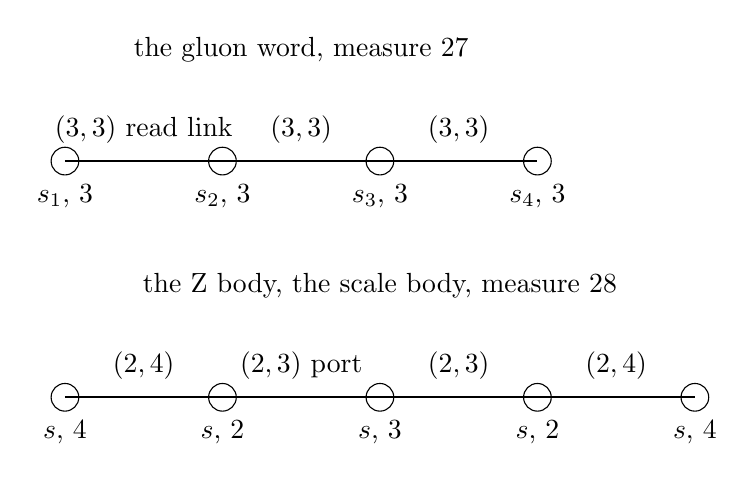
\begin{tikzpicture}[scale=1]
\foreach \x in {0,2,4,6} {\filldraw[fill=white] (\x,0) circle (5pt);}
\draw[thick] (0,0) -- (6,0);
\node at (0,0) [below=5pt] {$s_1$, 3}; \node at (2,0) [below=5pt] {$s_2$, 3}; \node at (4,0) [below=5pt] {$s_3$, 3}; \node at (6,0) [below=5pt] {$s_4$, 3};
\node at (1,0) [above=3pt] {$(3,3)$ read link}; \node at (3,0) [above=3pt] {$(3,3)$}; \node at (5,0) [above=3pt] {$(3,3)$};
\node at (3,1) [above=4pt] {the gluon word, measure $27$};
\foreach \x/\d in {0/4,2/2,4/3,6/2,8/4} {\filldraw[fill=white] (\x,-3) circle (5pt); \node at (\x,-3) [below=5pt] {$s$, \d};}
\draw[thick] (0,-3) -- (8,-3);
\node at (1,-3) [above=3pt] {$(2,4)$}; \node at (3,-3) [above=3pt] {$(2,3)$ port}; \node at (5,-3) [above=3pt] {$(2,3)$}; \node at (7,-3) [above=3pt] {$(2,4)$};
\node at (4,-2) [above=4pt] {the Z body, the scale body, measure $28$};
\end{tikzpicture}\caption{The gluon word with its (3,3) read link and the Z body through which the read is carried by the scale map, with its port.}\end{figure}
\end{chproof}
\par\medskip\noindent{\itshape The carrier of the Part, the photon, is read in the next chapter.}\label{narr:close:5-7}\par
\section{The photon: docking, the join face and pair production}\label{mod:V-8-photon-docking-the-join-face-and-pair-production}
\chdesig{7-8}{5-8}{V-8-photon-docking-the-join-face-and-pair-production}{V-8-D539949-phpk-t1}
\label{narr:open:5-8}Theorem~150.1 reads the photon as docking at both faces, with pair production at the join face, resting on the link, the moves, the saturation, the probe, the constant and the hydrogen chapter.
\begin{chconditional}[The photon docks at both faces]\label{box:V-8-photon-docking-the-join-face-and-pair-production:1}
This result is conditional on the axiom text and on the results of the chapters named as its premises in the derivation below, each at its own standing.
The photon word of the construction, held at both of its ends under the docking act of the axiom text, the qutrit end at the electron dock and the qubit end at the up core by two qutrit-qubit pairs, docks at both of its faces, and the join face that the carrier read of the read link posed as its condition is derived at the dock, the spin content of the read a two-dimensional representation (the doublet).
\end{chconditional}
\chstanding{a conditional theorem}
\chdeps{Definitions 1.1 to 1.6, Theorems 9.1 to 9.7 and Open result 9.8, Theorems 28.1 and 28.2, Open results 28.3 and 28.4 and Theorem 28.5, Theorem 124.1, Theorem 143.1, Open results 241.1 and 241.2, Theorems 241.3 and 241.4 and Open results 241.5 to 241.7 and Open results 245.1 and 245.2, Theorem 245.3, Open results 245.4 to 245.8 and Theorem 245.9}{Theorem 151.1 and Theorem 226.1 and Open result 226.2}
The join face of the photon as the record carries it, the glossary entry of the photon-electron vertex at its typing result, equals the pairing move of the move table applied at the photon, so the join face is the pairing move and no posed face.
Two open results stand here. The closure at the docking face is not derived from the definition of open at the first rung, the parting named at the first test with both faces printed. The hub-forming move of the move table applied to the two standing photon words, the chain of six sites and five links with their open qubit ends paired, does not reach the electron-positron pair as the record carries it, so pair production as the hub-forming move parts as yet. A further open result placed here, the open count at the dock link, is cited at its own standing and compared with nothing.
\begin{chbridge}
The photon is the massless gauge boson of quantum electrodynamics, coupled to the electron current at the vertex $-ie\gamma^{\mu}$ with two transverse polarizations and no longitudinal one \cite{Peskin1995}; pair production in the field of a nucleus is the lowest-order process by which a photon of energy above twice the electron rest energy becomes an electron and a positron, its cross section given by Bethe and Heitler \cite{BetheHeitler1934}. The correspondence is by name.
\end{chbridge}
\begin{chproof}[exact part and census part]
The premises of this derivation are the axiom and the six definitions of chapter~\ref{mod:FRAMEWORK}, the theorem of chapter~\ref{mod:I-2-link-and-its-six-genres}, the theorem of chapter~\ref{mod:I-4-moves-in-one-table}, the theorem of chapter~\ref{mod:I-5-saturation-in-one-figure-seeds-waves-termination-sinks}, the theorem of chapter~\ref{mod:I-6-read-at-a-register-the-probe-and-the-measurement}, the theorem of chapter~\ref{mod:V-1-fine-structure-constant-at-the-one-link} and the theorem of chapter~\ref{mod:V-4-hydrogen-the-rydberg-ladder-and-the-fine-structure}. The chain of premises runs back to the axiom through those chapters, and the longest such chain in this compendium is twelve chapters long.
The held carrier of the hydrogen result is docked at both ends, the dock read of the electron and the up core taken at the qutrit and qubit ends, and the join face of the carrier read derived at the dock from the one-act clause and the join as a contraction of ket and bra ends; the join face is stated from the glossary entry and the typing result, the pairing move of the move table computed at the photon and the two compared. The docking theorem is conditional on the open results it rests on, among them the star as the electron dock read and spin as the doublet content of the read; the join-face theorem rests on the axiom text and the proved results it names alone.
\textit{The exact part.}
From the photon word held at both ends under the docking act (the qutrit end at the electron dock and the qubit end at the up core by two qutrit-qubit pairs), by the two dockings the hydrogen result admits, we obtain the exchange at the two-qubit type hosted at the first dock qubit of the electron with the odd cycle of length two, the mass face at the join six root six against the standing mass face thirty-six.
\begin{equation}
\text{exchange type } (2,2) \ \text{at the host } w_{1}, \qquad M_{\mathrm{join}} = 6\sqrt{6}, \qquad M_{\mathrm{standing}} = 36 .
\end{equation}
From the one-act clause and the join as a contraction of ket and bra ends, by the two-qubit join at the electron dock, we obtain the join face the carrier read posed as its condition, derived at the dock at every one of its thirty-one cells, the spin content of the read a two-dimensional representation.
\begin{equation}
\text{join face} = \text{the } (2,2) \text{ join at the electron dock}, \qquad \dim(\text{spin content}) = 2 .
\end{equation}
\textit{The census part.}
By exhaustive enumeration of the two dockings of the photon word the hydrogen result admits, each built as an exact object under both acts of the derived docking, the photon docks at both of its faces, the dock read of the electron and the up core is taken at the qutrit and qubit ends, the join face of the carrier read is derived at the dock from the one-act clause and the join as a contraction, and the thirty-one cells of the posed join face are re-met at every one. The join face as the glossary entry of the photon-electron vertex carries it equals the pairing move of the move table applied at the photon. The smallest case, the docking at the electron dock, is worked above.
The counter-tests alter the objects singly and read what moves. Docking at one face alone moves the dock, bind, spin and join cells from yes to no with the exchange undefined and the join mass face undefined. The five counter-tests stand at their pinned letters and the sixteen controls read the same at both engines, among them the construction, the figures and the register rule. The result was reproduced by a second engine built apart from the first, the two runs equal at every key.
The machine-checked package named at the reproducibility appendix certifies the statements of this chapter under the definitions of this compendium.
\chcert{31}
\end{chproof}
\begin{figure}[h]\centering
\setlength{\unitlength}{1pt}
\begin{picture}(260,150)
\qbezier(83.4,68.6)(103.5,48.5)(123.6,28.4)
\put(109.2,54.2){\makebox(0,0){\scriptsize $(2,3)$}}
\qbezier(136.4,121.6)(156.5,101.5)(176.6,81.4)
\put(162.2,107.2){\makebox(0,0){\scriptsize $(2,2)$}}
\qbezier(123.6,121.6)(103.5,101.5)(83.4,81.4)
\put(109.2,95.8){\makebox(0,0){\scriptsize $(2,3)$}}
\put(130.0,128.0){\circle{14}}
\put(130.0,128.0){\makebox(0,0){\footnotesize $2$}}
\put(130.0,138.0){\makebox(0,0)[b]{\scriptsize $s_1$}}
\put(77.0,75.0){\circle{14}}
\put(77.0,75.0){\makebox(0,0){\footnotesize $3$}}
\put(77.0,85.0){\makebox(0,0)[b]{\scriptsize $s_6$}}
\put(130.0,22.0){\circle{14}}
\put(130.0,22.0){\makebox(0,0){\footnotesize $2$}}
\put(130.0,32.0){\makebox(0,0)[b]{\scriptsize $w_1$}}
\put(183.0,75.0){\circle{14}}
\put(183.0,75.0){\makebox(0,0){\footnotesize $2$}}
\put(183.0,85.0){\makebox(0,0)[b]{\scriptsize $Q_1$}}
\end{picture}
\caption{The photon word docked at both faces, its qutrit end at the electron dock qubit and its qubit end at the up core, drawn at its two end sites. The two-qubit join at the electron dock supplies the join face of this chapter.}
\end{figure}
\section{The photon as the (2,2) pair ket at the join}\label{mod:V-8-D539949-phpk-t1}
\begin{chtheorem}[The photon as the (2,2) pair ket at the join]\label{box:V-8-D539949-phpk-t1:1}
The office of the (2,2) pair ket at the join under the body-alone rule is zero. The pair ket at the join, a word of two qubit sites and one (2,2) link, the contraction of the pairing move at the qubit ends of two photon reads, the pair of the hub unit and the carrier genre of the electromagnetic, located at four of four parents, is a pendant pair in the dock set of the rule, its act struck at the reading adopted, so its first power is zero, equal to the established first power of the closed read of the photon at the carrier-mass result, its pair part is zero, equal to the first power squared, its closure is zero at its one dark link, and its office is the exact cell zero, the smallest office among the eighteen established offices and equal to the photon object office of the carrier-mass result at both faces and below every other. The genre is bright at the readability result at order one at three faces and the deciding cell, and the two move classes of the electromagnetic, the hub-forming pairing at sixteen edges and the (2,2) join across webs at 31325 edges, are re-met at the forces result with the carrier genre (2,2) at two of two.
The first face, the office of the (2,2) pair ket at the join under the body-alone rule a cell read at order one as a bright genre with its two move classes re-met, the cell zero or the smallest office, reads yes at the reading adopted, located four of four, bright, the office zero and exact with the identity, the smallest, the classes re-met two of two; the second face, the rule refusing a word at the bright genre or the pair ket at the join no word of the construction, reads no, the rule refusing the word at no cell, the pair ket located at every parent and at the fixed library of webs, the first parting none.
\end{chtheorem}
\chstanding{a theorem}
\chdeps{Definitions 1.1 to 1.6 and Theorem 150.1}{no theorem beyond it at this release}
The pair ket at the join is the smallest word of the model that carries the electromagnetic, two qubit sites joined by one (2,2) link of measure four. Under the body-alone rule a link that is a pendant pair at a qubit end belongs to the dock set and its act is struck, so nothing is read along the one link of the word. The first power, the sum of the acts of the unstruck links, is zero. The pair part, the sum over ordered pairs of unstruck links, is zero and equals the square of the first power. The closure at the one dark link is its act multiplied by the link law of its genre, zero. The office, the sum of the three, is the exact cell zero. The same reading at the hub unit, at the pair ket with its two photon reads and at the other established words gives offices that are nonzero elements of the ring, so the office of the pair ket at the join is the smallest of them, and the carrier of the electromagnetic reads at order one as a bright genre whose two move classes are those the forces result names.
\begin{chbridge}
The photon is the massless gauge boson of electrodynamics, the quantum of the electromagnetic field, with zero rest mass and two polarization states, and its masslessness follows in the standard account from the unbroken gauge invariance of the theory \cite{Peskin1995,Weinberg1995}. The correspondence is by name.
\end{chbridge}
\begin{chproof}[finite computation with its exact part]
The premises of this derivation are the axiom and the six definitions of chapter~\ref{mod:FRAMEWORK}, the link and its six genres of chapter~\ref{mod:I-2-link-and-its-six-genres}, a theorem, the photon docking and the join face of chapter~\ref{mod:V-8-photon-docking-the-join-face-and-pair-production}, a theorem, the hub step of chapter~\ref{mod:VI-1-hub-step-as-the-weak-interaction}, a theorem, the mass unit and the first power of chapter~\ref{mod:VIII-1-mass-unit-and-the-first-power}, a theorem, and the body-alone office rule of chapter~\ref{mod:VIII-2-body-alone-office-rule}, a theorem. The chain of premises runs back to the axiom through those chapters, and the longest such chain in this compendium is twelve chapters long.
\textit{The object.} The pair ket at the join is the word of two qubit sites $k_1$ and $k_2$ and one link $k_1k_2$ of genre (2,2), the measure of the link $2\cdot 2=4$, built by the pairing move as the contraction of genre (2,2) at the qubit ends of two photon reads. It is located at four of four parents. At the hub step it stands as the one (2,2) line among the three unit lines $Kk_1$ at (2,4), $Kk_2$ at (2,4) and $k_1k_2$ at (2,2), the pair of the unit never split. At the photon join face it stands as the contraction at the dimensions two and two. At the forces result it stands as the carrier genre of the electromagnetic. At the fixed library of webs it stands as its (2,2) link. Its genre reads bright at order one at the readability result. The figure draws the word and the hub unit it sits in.
\textit{The procedure.} The reading adopted is the measure-struck read with the slot rule, the (3,4)-only dressing, the dark set at the first reading and the link-weight closure. For each link of a word decide whether it lies in the dock set of the rule, a pendant pair at a qubit end does. Strike the act of every dock link. Take the first power $S_1$ as the sum of the acts of the unstruck links, the pair part $P$ as the sum over ordered pairs of unstruck links of the product of their acts, and the closure $C$ as the sum over the dark links of the act multiplied by the link law of the genre. The office is $\Omega = S_1 + P + C$, an element of the ring with the basis one, root two, root three and root six.
\textit{The smallest instance.} The word has one link, $k_1k_2$, a pendant pair at both ends, hence in the dock set with its act struck. The link law of the (2,2) genre is $\tfrac{5}{216} + \tfrac{5}{216}\sqrt{2}$, and the act at the link is zero, so
\begin{equation} S_1 = 0, \qquad P = S_1^{2} = 0, \qquad C = 0\cdot\Big(\tfrac{5}{216} + \tfrac{5}{216}\sqrt{2}\Big) = 0, \qquad \Omega = 0 + 0 + 0 = 0 . \end{equation}
The first power zero equals the first power of the closed read of the photon at the carrier-mass result and its passage first power, both zero; the pair part equals the first power squared, an identity at every read of the grid; the closure is zero at the one dark link; and the office is the exact cell zero, rational, with the identity of the office and its parts holding.
\textit{The exact part.} The same rule at the nine reads of the grid gives the first powers and the offices listed below, each office an exact element of the ring written as its coefficients of one, root two and root three; the office of the pair ket at the join is the smallest, and it equals the photon object office of the carrier-mass result.
\begin{center}\begin{adjustbox}{max width=\linewidth}\begin{tabular}{lrl}\hline read & first power & office \\ \hline the pair ket at the join & 0 & $0$ \\ the pair ket with its two photon reads & 114 & $\tfrac{43118427966377}{3317760000} + \tfrac{649}{4050}\sqrt{2} + \tfrac{5069}{41472000}\sqrt{3}$ \\ the hub unit & 20 & $\tfrac{1458099887}{3645000} + \tfrac{649}{36450}\sqrt{2}$ \\ the photon read, its one (2,3) dock struck & 0 & $0$ \\ the photon word of the library, five (2,3) links & 24 & $576$ \\ the (2,4) free genre & 8 & $\tfrac{466566137}{7290000} + \tfrac{2}{6075}\sqrt{2}$ \\ the W word of the library & 28 & $\tfrac{2857690241}{3645000} + \tfrac{98}{50625}\sqrt{2}$ \\ the Higgs word of the library & 16 & $\tfrac{46656001681}{182250000}$ \\ the electron & 201 & the largest of the nine, at the table of the entry \\ \hline \end{tabular}\end{adjustbox}\end{center}
The two move classes of the electromagnetic at the forces result are the hub-forming pairing, present at sixteen edges with the carriers (2,2), (2,3), (2,4) and (3,4), and the (2,2) join across webs, present at 31325 edges with the carrier (2,2); both carry the genre of the object, both stand among the twenty-eight move ids, and the two re-meet the forces result at two of two.
\textit{The check.} The counter-tests alter the object singly and read what moves. Reading the pair ket at a dark genre, the second qubit struck to a ququart and the link read as (2,4) outside the dock set, gives the first power eight and a nonzero office, twenty cells moved. Keeping the pendant pair in the act read gives the first power four, thirteen cells moved. Striking the (2,2) join class from the located classes parts the re-meet at the count, nine cells moved. Striking the text unmeets the gate, every cell struck. Striking the deciding cell moves twenty-four cells. Each alteration moves the cells it names. The result was reproduced by an independent route, two engines built apart, the keyed-map and fraction route against the array-scan and closed-form route, equal at every cell, with the four control reads of the Higgs-and-carrier offices re-met at four of four and the sixteen controls the same.
\chcert{240}
\begin{figure}[h]\centering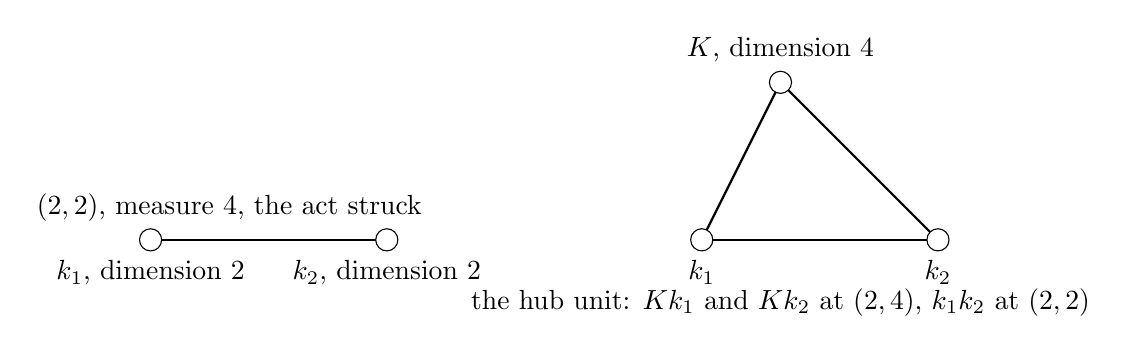
\begin{tikzpicture}[scale=1]
\draw[thick] (0,0) -- (3,0);
\filldraw[fill=white] (0,0) circle (4pt) node[below=4pt] {$k_1$, dimension 2};
\filldraw[fill=white] (3,0) circle (4pt) node[below=4pt] {$k_2$, dimension 2};
\node at (1,0) [above=3pt] {$(2,2)$, measure $4$, the act struck};
\draw[thick] (7,0) -- (10,0);
\draw[thick] (7,0) -- (8,2);
\draw[thick] (10,0) -- (8,2);
\filldraw[fill=white] (7,0) circle (4pt) node[below=4pt] {$k_1$};
\filldraw[fill=white] (10,0) circle (4pt) node[below=4pt] {$k_2$};
\filldraw[fill=white] (8,2) circle (4pt) node[above=4pt] {$K$, dimension 4};
\node at (8,0) [below=14pt] {the hub unit: $Kk_1$ and $Kk_2$ at $(2,4)$, $k_1k_2$ at $(2,2)$};
\end{tikzpicture}\caption{The pair ket at the join, two qubit sites and one (2,2) link, and the hub unit in which it stands as the one (2,2) line.}\end{figure}
\end{chproof}
\par\medskip\noindent{\itshape The next chapter concerns the equation of the charged body at the dock, and is counted empty.}\label{narr:close:5-8}\par
\section{The lepton ladder as hub assemblies}\label{mod:V-10-lepton-ladder-as-hub-assemblies}
\chdesig{7-10}{5-10}{V-10-lepton-ladder-as-hub-assemblies}{V-10-D540869-tthc-t1}
\label{narr:open:5-10}Theorem~152.1 reads the lepton ladder as hub assemblies, resting on the moves, the saturation and the mass unit of chapter 8-1.
\begin{chconditional}[The lepton ladder as hub assemblies]\label{box:V-10-lepton-ladder-as-hub-assemblies:1}
This result is conditional on the axiom text and on the results of the chapters named as its premises in the derivation below, each at its own standing.
At every one of the three lepton webs of the construction the unstruck links are the three coloured core links plus $k$ hub assemblies, each one in-leg, three qubit-ququart legs and one qubit pair at the measure forty, the electron at $k$ one, the muon at two and the tau at three, so the first powers of the ladder are one measure law at three terms.
\end{chconditional}
\chstanding{a conditional theorem}
\chdeps{Definitions 1.1 to 1.6, Theorems 185.1 to 185.12, Open results 241.1 and 241.2, Theorems 241.3 and 241.4 and Open results 241.5 to 241.7 and Open results 245.1 and 245.2, Theorem 245.3, Open results 245.4 to 245.8 and Theorem 245.9}{the theorems of Chapters 1-5, 7-10 to 7-12, 8-2b, 10-1, 10-3 to 10-5, 14-1, 14-6}
The electron body is read by the same rule as every other body and that rule reads it at its hub: the rank of a body, the sum over its links of the end products with the attachments struck, is sixty-seven at the electron, and the read multiplies that rank by its hub product, three at the electron, so the unit of the mass readout stands at 201 at the hub reading and 67 at the dock reading, the two offices parted by the factor nine at every body.
The standing hub step keeps both docks of the electron at both steps, and the muon and tau of the construction are exactly the dock-freed pair readings at the core, every other lowering of the electron isomorphic to none of the lowering classes of the closure of the construction.
With every record of the joined webs of the electron and muon results re-cut at the three record classes of the placement theorem (the position of a tensor in a network), the body-part ratio of the muon to the electron is defined, its interference term an exact nonzero element of the field with a definite sign.
At every qutrit-qubit link of the construction whose qutrit site is the in-end of a qutrit-ququart hub leg, the qutrit end is open as the far end of its hub leg under the definition of open, so the hub leg opens the qutrit end the dock rule closes.
Four open results stand here. The hub as the pair read as one qudit preserves the dressing but consumes the three links of the triangle. The joined read at the ladder of the construction is defined at the electron and the muon and refused at the tau, whose standing attach site is closed. The one rule of the item, the Born count at the open-end set less the struck-dock term multiplied by the hub-leg product, is not the ladder, parting at the muon and the tau. The hub-attached three-quark web read under one rule parts at its first named web. A further open result placed here, every lepton office at its whole sink, is cited at its own standing.
\begin{chbridge}
The three charged leptons of the Standard Model carry the same charge and couplings and differ in mass alone, the three masses three Yukawa couplings fixed by measurement \cite{Weinberg1967}; the generation count three is an input of the model. The correspondence is by name; the record supplies an isometry algebra of the Hermitian split at the Lorentz brackets, a lattice point group, boosts from the order register and a transverse traceless part at the open read, every one a finite or algebraic object of this theory carrying the group name at chapter~\ref{mod:III-2-rotation-group}, chapter~\ref{mod:III-3-lorentz-group-and-the-signature}, chapter~\ref{mod:III-4-boosts-and-the-one-unit}, chapter~\ref{mod:III-5-spin-and-helicity}, the chapter titled Causal structure and general covariance (chapter~\ref{mod:III-8-causal-structure-and-general-covariance}, among the instruments) and chapter~\ref{mod:XIV-7-what-remains-the-ungraded-page}, and the mass corresponds there and here by name.
\end{chbridge}
\begin{chproof}[exact part and census part]
The premises of this derivation are the axiom and the six definitions of chapter~\ref{mod:FRAMEWORK}, the theorem of chapter~\ref{mod:I-4-moves-in-one-table}, the theorem of chapter~\ref{mod:I-5-saturation-in-one-figure-seeds-waves-termination-sinks} and the theorem of chapter~\ref{mod:VIII-1-mass-unit-and-the-first-power}. The chain of premises runs back to the axiom through those chapters, and the longest such chain in this compendium is twelve chapters long.
The rank is summed over the links with the attachments struck and the hub product taken; the two-step readings of the hub step are enumerated at every pure attachment site; the records of the joined webs are re-cut at the three record classes; every qualifying link is typed at the definition of open; and the unstruck links of the three lepton webs are listed and re-met as sets. The body-read theorem is conditional on the open results it rests on, among them the hub dressing at the body; the others rest on the axiom text alone.
\textit{The exact part.}
From the electron web, by listing its unstruck links, we obtain the core triangle of three colored links at the measure twenty-seven and one hub assembly, the in-leg of measure twelve, three qubit-ququart legs of measure twenty-four together and one qubit pair of measure four, the assembly at the measure forty. The two dock links of the qutrit-qubit type are struck at the measure twelve, so the measure and the rank are
\begin{equation}
27 + 40 + 12 = 79, \qquad \operatorname{rank}(e) = 79 - 12 = 67 .
\end{equation}
From the muon and tau webs, by the same listing, we obtain the core triangle plus two and three hub assemblies, the struck docks at measures six and zero and the struck two-qubit leaf links at four and eight, so the measures step as
\begin{equation}
27 + 2 \cdot 40 + 6 + 4 = 117, \qquad 27 + 3 \cdot 40 + 0 + 8 = 155, \qquad \operatorname{rank}(\mu) = 107, \quad \operatorname{rank}(\tau) = 147 ,
\end{equation}
the ranks stepping by forty at both steps, equal to the hub-assembly measure, so the first powers of the ladder are one measure law at three terms.
\begin{equation}
\operatorname{rank}(\ell_{k}) = 27 + 40\,k, \qquad k = 1, 2, 3 .
\end{equation}
\textit{The census part.}
By exhaustive enumeration of the links of the three lepton webs of the construction at both readings of the docks, every unstruck link is assigned to the core triangle or to one hub assembly (each one in-leg, three qubit-ququart legs and one qubit pair at the measure forty) with no link assigned to none at either reading, the electron at one assembly, the muon at two and the tau at three. The rank is summed over the links with the attachments struck and the hub product taken, and the first powers of the ladder re-met as sets. The smallest case, the electron web, is worked above.
The counter-tests alter the objects singly and read what moves. Striking one assembly moves all nine of its cells, the first the dock of the electron. The four counter-tests stand at their pinned letters and the ten controls read the same at both engines, every consumed file unaltered. The result was reproduced by a second engine built apart from the first, the two runs equal at every one of the cells of both.
The machine-checked package named at the reproducibility appendix certifies the statements of this chapter under the definitions of this compendium.
\chcert{3}
\end{chproof}
\begin{figure}[h]\centering
\setlength{\unitlength}{1pt}
\begin{picture}(260,150)
\qbezier(121.5,124.9)(113.0,121.8)(104.4,118.7)
\put(115.7,114.3){\makebox(0,0){\scriptsize $(3,3)$}}
\qbezier(91.4,107.8)(86.9,99.9)(82.3,92.0)
\put(93.8,95.9){\makebox(0,0){\scriptsize $(3,3)$}}
\qbezier(84.7,90.0)(103.9,106.1)(123.1,122.2)
\put(98.8,112.2){\makebox(0,0){\scriptsize $(3,3)$}}
\qbezier(88.6,56.3)(107.1,88.2)(125.5,120.2)
\put(100.1,92.2){\makebox(0,0){\scriptsize $(3,4)$}}
\qbezier(91.0,42.7)(98.0,36.8)(105.0,31.0)
\put(103.1,43.0){\makebox(0,0){\scriptsize $(2,4)$}}
\qbezier(92.6,45.4)(116.1,36.8)(139.7,28.3)
\put(118.9,44.4){\makebox(0,0){\scriptsize $(2,4)$}}
\qbezier(93.1,48.5)(130.0,48.5)(166.9,48.5)
\put(130.0,56.5){\makebox(0,0){\scriptsize $(2,4)$}}
\qbezier(120.9,25.2)(130.0,25.2)(139.1,25.2)
\put(130.0,33.2){\makebox(0,0){\scriptsize $(2,2)$}}
\qbezier(104.4,112.5)(139.1,99.9)(173.7,87.3)
\put(141.8,107.4){\makebox(0,0){\scriptsize $(2,3)$}}
\qbezier(86.3,87.3)(120.9,99.9)(155.6,112.5)
\put(118.2,107.4){\makebox(0,0){\scriptsize $(2,3)$}}
\put(130.0,128.0){\circle{14}}
\put(130.0,128.0){\makebox(0,0){\footnotesize $3$}}
\put(130.0,138.0){\makebox(0,0)[b]{\scriptsize $A$}}
\put(95.9,115.6){\circle{14}}
\put(95.9,115.6){\makebox(0,0){\footnotesize $3$}}
\put(95.9,125.6){\makebox(0,0)[b]{\scriptsize $B$}}
\put(77.8,84.2){\circle{14}}
\put(77.8,84.2){\makebox(0,0){\footnotesize $3$}}
\put(77.8,94.2){\makebox(0,0)[b]{\scriptsize $C$}}
\put(84.1,48.5){\circle{14}}
\put(84.1,48.5){\makebox(0,0){\footnotesize $4$}}
\put(84.1,58.5){\makebox(0,0)[b]{\scriptsize $H$}}
\put(111.9,25.2){\circle{14}}
\put(111.9,25.2){\makebox(0,0){\footnotesize $2$}}
\put(111.9,35.2){\makebox(0,0)[b]{\scriptsize $g_1$}}
\put(148.1,25.2){\circle{14}}
\put(148.1,25.2){\makebox(0,0){\footnotesize $2$}}
\put(148.1,35.2){\makebox(0,0)[b]{\scriptsize $g_2$}}
\put(175.9,48.5){\circle{14}}
\put(175.9,48.5){\makebox(0,0){\footnotesize $2$}}
\put(175.9,58.5){\makebox(0,0)[b]{\scriptsize $g_3$}}
\put(182.2,84.2){\circle{14}}
\put(182.2,84.2){\makebox(0,0){\footnotesize $2$}}
\put(182.2,94.2){\makebox(0,0)[b]{\scriptsize $w_1$}}
\put(164.1,115.6){\circle{14}}
\put(164.1,115.6){\makebox(0,0){\footnotesize $2$}}
\put(164.1,125.6){\makebox(0,0)[b]{\scriptsize $w_2$}}
\end{picture}
\caption{The electron web as the core triangle plus one hub assembly, the three qutrit core sites, the hub of dimension four with its in-leg, its three qubit legs and the qubit pair, and the two dock qubits whose links are struck. Each site labeled by its dimension and each link by its pair type.}
\end{figure}
\section{The lepton block at the unwashed port overlap}\label{mod:V-10-D539519-w-tflb}
The mixing of the three lepton generations is a unitary three-by-three block relating the flavour states to the mass states of the neutral partners, parametrised by three angles and a phase, its single rephasing-invariant measure of CP violation the Jarlskog invariant; the block is unitary on three when the neutral partners are three alone, and a fourth column would mark a further state \cite{Pontecorvo1958,Maki1962,Jarlskog1985}. The lepton ladder as hub assemblies is introduced at section~\ref{mod:V-10-lepton-ladder-as-hub-assemblies} and the mixing with the washed overlap at section~\ref{mod:VI-7-mixing-the-washed-overlap-and-the-ckm-block}.
The three-by-three block of the lepton overlap at the three read sites, with the dark end as a fourth column, is cut unwashed at the open ports: the dock read of the charged partner against the port read at the hub register, every far end of the hub open at the hub read at 20 of 20 letter and far-end pairs, the frame test and the dimension test agreeing, and the wash applied at no open port. Cut at every one of the six hub assemblies of the standard lepton webs and every one of the 20 letter pairs, the unwashed block is unitary at the base criterion at 4 of 20 pairs and flat at 7 of 20.
The six assemblies are lined up with the three cross-core webs by the hub count at 3 of 3. Among the 20 pairs one block is a unitary with distinct moduli, the Jarlskog cell is nonzero at none of them and a single value at 9 of 20, and the block phases fall inside the phase group of the (3,3) genre at 76 of 165 with the cycles exact at 9 of 20. The washed block of the standing result, unitary at 0 of 20 and flat at 20 of 20, the unread-end reading, unitary at 4 of 20, and the port-typed reading each stand at their own second face. The first parting is the first assembly, the electron hub at the letter pair Z against X with the dark-end column at the third leg: there the block is flat and not unitary, its Born block one quarter at every entry with the row sums three quarters, its Gram matrices parting from the identity, and its Jarlskog cell one sixteenth with the square 1 over 256; the second value named is the first block phase outside the phase group. Two independent implementations agree at every value and the runs are byte-identical.
The result is an open one, an open result: the stronger statement, that the unwashed block at the open ports is unitary on three, is not met, and the weaker statement is named with both values; no comparison with observation is made here.
What stays open is the reading of this block together with the washed block carrying the dark-end column (section~\ref{mod:VI-7-D539152-w-lmde}) and with the muon ports under the derived definition (the chapter titled The muon ports under the derived definition of open (chapter~\ref{mod:VI-2a-D539543-mprt-t1}, among the instruments)), which no result has made.
\section{The tau as the third hub on the triangle core}\label{mod:V-10-D540869-tthc-t1}
\begin{chtheorem}[The tau as the third hub on the triangle core]\label{box:V-10-D540869-tthc-t1:1}
The tau as the third hub on the triangle core, at its second face: no isomorph of the triangle-plus-one web built from the muon web of the fixed library stands among the three hundred three-hub lepton-form sinks of the tau census, zero of three hundred at the reading adopted, at the leaf reading and at the star reading; its own Koide ratio at the first powers lies outside the band of one part in a thousand of two thirds, 9336401 over 13739282 at the first power 4212, as does every one of the three hundred, zero of three hundred inside; the nearest candidate of the triangle-plus-one kind is the sink at the first power 3996 and the ratio 8449937 over 12630338, the nearest of the star kind the tau sink itself at 4185 and 18446083 over 27196225; so the second face holds, absent or outside with the nearest candidates named with both cells, and the first face fails, every cell an exact element of the ring compared with the canonical two thirds alone.
The first face, an isomorph of the triangle-plus-one web present among the three hundred with its Koide ratio inside the band, reads no, no isomorph present and none inside; the second face, absent or outside with the nearest candidates named, reads yes at the first basis of the search, the isomorphism absent at zero of three hundred and the ratio outside at every sink.
\end{chtheorem}
\chstanding{a theorem}
\chdeps{Definitions 1.1 to 1.6 and Theorem 152.1}{no theorem beyond it at this release}
The question was whether the tau is the muon web grown by one more hub on its triangle core, the third generation as the third hub. The web that reading builds, eighteen sites and twenty-one links with three hubs of degree four on a core of four qutrits, is compared site by site and link by link with every three-hub lepton-form sink of the tau census, and none of the three hundred is that web under any bijection of sites that keeps the dimensions and the genres of the links; the tau sink identified by the identification standard, a star core of sixteen sites, is not that web either. The Koide ratio, the sum of the squares of the three first powers over the square of their sum with the electron at 67 and the muon at 963, is an exact rational at every sink, and it lies outside a band of one part in a thousand around two thirds at every one of them and at the triangle-plus-one web itself, so the reading supplies neither the tau nor the Koide relation, and the result names the nearest candidates of each core kind with both of their cells.
\begin{chbridge}
The tau is the third charged lepton, the heaviest of the three generations, and the Koide relation is the empirical statement that the sum of the three charged-lepton masses is two thirds of the square of the sum of their square roots, a relation with no derivation in the Standard Model, where the lepton masses are Yukawa couplings fixed by measurement \cite{Koide1983,Weinberg1995}. The correspondence is by name.
\end{chbridge}
\begin{chproof}[finite computation]
The premises of this derivation are the axiom and the six definitions of chapter~\ref{mod:FRAMEWORK}, the lepton ladder as hub assemblies of chapter~\ref{mod:V-10-lepton-ladder-as-hub-assemblies}, a theorem, the body-alone office rule of chapter~\ref{mod:VIII-2-body-alone-office-rule}, a theorem, the dressing as the unpassed (3,4) in-legs of chapter~\ref{mod:VIII-1-mass-unit-and-the-first-power}, a theorem, and the Koide class of chapter~\ref{mod:V-12-koide-class}, an open result. The chain of premises runs back to the axiom through those chapters, and the longest such chain in this compendium is twelve chapters long.
\textit{The procedure.} The input objects are the generation-step web, built from the muon web of the fixed library by keeping its triangle core, placing a fourth qutrit on the corner and attaching a third hub with its legs as the first muon hub carries them, and the three hundred three-hub lepton-form sinks of the tau census, each located at its state row by face, wave and id in the seven state files of that census. For every sink the census cells, the sites, links, measure, docks and hubs, are re-read and the core kind, the dock count, the in-leg count, the dressing, the rank, the first power at the wave-zero reading of the body-alone rule and the office are computed. The test applied to each sink is twofold: whether some bijection of its sites onto the sites of the generation-step web preserves the dimension of every site and the genre-labeled adjacency of every link, searched depth first by the first engine and by backtracking placement by the second, at three readings of the third hub; and whether its Koide ratio lies within one part in a thousand of two thirds. The aggregation counts the isomorphs and the sinks inside the band and names the nearest candidate of each core kind by its distance.
\textit{The objects at their cells.} The generation-step web has 18 sites, 11 qubits, 4 qutrits and 3 ququarts, 21 links at the genres (2,2) four, (2,3) one, (2,4) nine, (3,3) four and (3,4) three, the measure 166, three hubs of degree four, three in-legs and the dressing 27, one dock at the first reading and the dock set of measure 10, the core of four qutrits on four (3,3) links, the rank 156 and the first power 4212. The three hundred sinks fall into the core kinds star 88, triangle-plus-one 87, four-cycle-plus-one 0 and other 125, the last being 114 triangles and 11 three-qutrit paths; their dressings are 3 at 199 sinks, 9 at 88 and 27 at 13, and their first powers run from 369 to 4617 at 63 distinct values.
\textit{The smallest instance.} The Koide ratio at the generation-step web itself, with the electron and the muon first powers 67 and 963 and its own first power 4212, is
\begin{equation} \frac{67^{2} + 963^{2} + 4212^{2}}{(67 + 963 + 4212)^{2}} = \frac{4489 + 927369 + 17740944}{5242^{2}} = \frac{18672802}{27478564} = \frac{9336401}{13739282}, \end{equation}
and its distance from two thirds is
\begin{equation} \frac{2}{3} - \frac{9336401}{13739282} = \frac{27478564 - 28009203}{41217846} = -\frac{530639}{41217846}, \end{equation}
outside the band, since one part in a thousand of two thirds is 1 over 1500 and 530639 over 41217846 exceeds it. The same arithmetic at the sink of the triangle-plus-one kind with the first power 3996 gives the ratio 8449937 over 12630338 at the distance 89135 over 37891014, the nearest overall, and at the tau sink of the star kind with the first power 4185 the ratio 18446083 over 27196225 at the distance 945799 over 81588675, both outside.
\textit{The result.} The isomorphism search finds the generation-step web present at 0 of 300 at the reading adopted, 34 sinks sharing its site and link counts and none a map, at 0 of 300 at the leaf reading, 41 at its counts, and at 0 of 300 at the star reading, 6 at its counts; the tau sink of sixteen sites parts from the web at the site counts, 16 against 18, with zero maps at every reading. The control pairs re-meet the identity engines, the electron sink onto the two-dock web the same at four maps, the muon sink onto the muon web the same at four maps, and the tau sink against the tau web parting at zero maps. The sinks inside the band number 0 of 300. So the second face holds and the first fails, and the theorem states the second face with the nearest candidates named.
\textit{The check.} The counter-tests alter the inputs singly and read what moves. Replacing the generation-step web by the tau web of the fixed library at the search moves the site count of the search. Widening the band to one part in ten moves the count of sinks inside. Replacing the reference first powers by the body-alone first powers of the library webs moves the Koide cells. Striking the text unmeets the gate. Each alteration moves the cells it names. The result was reproduced by an independent route, two engines built apart, the depth-first search against the backtracking placement, equal at every cell, the two-read identity re-met at nine of nine reads and three hundred of three hundred sinks and the fourteen controls the same.
\chcert{300}
\end{chproof}
\par\medskip\noindent{\itshape The ladder in hand, the next chapter reads the dissolution of a face and the exponent it leaves.}\label{narr:close:5-10}\par
\section{The face dissolution, the leg count and the exponent}\label{mod:V-11-face-dissolution-the-leg-count-and-the-exponent}
\chdesig{7-11}{5-11}{V-11-face-dissolution-the-leg-count-and-the-exponent}{V-11-D543290-w-grfn}
\label{narr:open:5-11}Theorem~155.1 is the face dissolution theorem, with the leg count and the exponent, resting on the mass unit and the lepton ladder.
\begin{chconditional}[The face dissolution theorem]\label{box:V-11-face-dissolution-the-leg-count-and-the-exponent:1}
This result is conditional on the axiom text and on the results of the chapters named as its premises in the derivation below, each at its own standing.
The two readings of the mass law, the dock reading and the hub reading, are one law up to the unit absorbing one leg at every established result, the ratio form carries no reading, and the reading word is dissolved with its residue the leg function as a corollary.
\end{chconditional}
\chstanding{a conditional theorem}
\chdeps{Definitions 1.1 to 1.6, Theorem 152.1 and Theorems 185.1 to 185.12}{Open result 156.1 and Theorems 198.1 to 198.3 and Open results 198.4 and 198.5}
The standing two-dock act, named from the electron of the construction, its two docks and its hub with the carry from the hub reaching both docks at once as the far ends, transported to the two-port neutral object reaches every cross-core port, all six at the three cross-core webs and all twenty at the ten objects, and names the reading by the arrows alone at all three generations, the same reading at the first and the third and the opposite at the second.
The in-leg count is one function of the web alone, invariant under every reading and equal to the established $k$ at every result, so the leg count is a definition, the two open questions of the reading dissolved as questions of the reading and the first-power law carrying $k$ by construction.
Four open results stand here. The result that fixes the arrows at the fourteen sinks of the pairing move reaches no port of the three cross-core webs, so the face at the cross-core ports is undefined at those arrows at all three generations. The generator of the step (the step generator) at the first parting tabulated link parts from the factor six multiplied by the order operator lifted to the link register, the first parting register the one link itself. The strike rule that a dock is struck exactly when it is the probe attach site reproduces the struck set at no tabulated lepton result. The probe read placed at the attach dock and carried through the web enters a hub through its qutrit at some webs and through a qubit copy at others, so the leg count read by the act is free at the first web named. Two further open results placed here, the strike as a sector and the strike rule per body at the typed cap, are cited at their own standing and compared with nothing.\textsuperscript{,}
\begin{chbridge}
In the Standard Model a mass term is written once, at the Lagrangian, and carries no choice of reading: the fermion mass is the coefficient of the bilinear in the field and its conjugate, the same number at every frame and at every basis of the fields \cite{Weinberg1967}, and the exponent of the mass in an amplitude is fixed by the dimension of the operator and by nothing else. The correspondence is by name; the record supplies a finite re-matching group at the known clause, a representation census at the open ends and the sinks, an attach-site basis carrying the generation name and a sink class carrying the doublet name at chapter~\ref{mod:IV-1-gauge-invariance-as-the-known-clause}, chapter~\ref{mod:IV-3-representations-from-the-open-end-census}, chapter~\ref{mod:IV-4-cartan-weights-and-the-charge}, chapter~\ref{mod:IV-6-conservation-as-the-kernel-of-the-move-matrix}, chapter~\ref{mod:IV-7-noether-at-the-sinks-and-the-kernel-identification}, chapter~\ref{mod:IV-9-one-rule-of-a-read-and-the-word-table}, chapter~\ref{mod:VI-3-doublets-handedness-and-parity-violation}, chapter~\ref{mod:VII-7-quark-content-and-flavour}, chapter~\ref{mod:VIII-4-three-generations-as-attach-sites} and chapter~\ref{mod:XIV-7-what-remains-the-ungraded-page}, and the generation count and the generation correspond there and here by name.
\end{chbridge}
\begin{chproof}[exact part, finite part and census part]
The premises of this derivation are the axiom and the six definitions of chapter~\ref{mod:FRAMEWORK}, the theorem of chapter~\ref{mod:VIII-1-mass-unit-and-the-first-power} and the theorem of chapter~\ref{mod:V-10-lepton-ladder-as-hub-assemblies}. The chain of premises runs back to the axiom through those chapters, and the longest such chain in this compendium is twelve chapters long.
The two-dock act is named from the electron of the construction, transported to the two-port neutral object and carried to every cross-core port with the reading read off the arrows at every generation; the dock reading and the hub reading of the mass law are compared at every established result; and the in-leg count is computed as a function of the web alone at every reading and re-met at the established $k$; every theorem rests on the axiom text and the proved results it names alone, and the open results are readings the derivation tried and parted at their named steps.
\textit{The exact part.}
From the two readings of the mass law at the electron, the dock reading at the dock-struck first power sixty-seven and the hub reading at the hub first power two hundred and one, by the ratio of the two units, we obtain the parting three at the first power and nine at the square, equal to the hub unit over the dock unit and its square, the unit absorbing one leg and nothing else, the electron at one over one at either face.
\begin{equation}
\frac{201}{67} = 3, \qquad \Big(\frac{201}{67}\Big)^{2} = 9, \qquad r_{e}^{\mathrm{dock}} = r_{e}^{\mathrm{hub}} = \tfrac{1}{1} .
\end{equation}
From every established cell of the parent results typed to its face (the dock face the row at the measure multiplied by three to the power $k$ over sixty-seven, the hub face at three to the power $k$ plus one over two hundred and one, the mixed face the hub numerator over the dock unit), by the computed cell against the established cell, we obtain equality at every one, so the two readings are one law up to the unit absorbing one leg.
\begin{equation}
\text{dock: } \frac{M \cdot 3^{k}}{67}, \qquad \text{hub: } \frac{M \cdot 3^{k+1}}{201}, \qquad \frac{M \cdot 3^{k+1}}{201} = \frac{M \cdot 3^{k}}{67} .
\end{equation}
\textit{The finite part.}
The procedure. Name the two-dock act from the electron of the construction, its two docks and its hub with the carry from the hub reaching both docks at once as the far ends. Transport it to the two-port neutral object and carry it to every cross-core port, reading the reading off the arrows at every generation. Compare the dock reading and the hub reading of the mass law at every established cell of the parents, typed to its face, and compute the in-leg count as a function of the web alone at every reading and re-meet it at the established $k$. The smallest instance, the electron at both faces, is worked above, the fifty established cells of the parents are typed to their faces and the computed cell equals the established cell at every one, the in-leg count one at the electron, two at the muon and three at the tau.
\textit{The census part.}
By exhaustive enumeration of the cross-core ports of the three cross-core webs (six) and of the ten objects (twenty), the transported two-dock act reaches every port and names the reading by the arrows alone at all three generations, the same reading at the first and the third and the opposite at the second. The leg count is one function of the web alone, invariant under every reading.
The counter-tests alter the objects singly and read what moves. The hub unit taken at two legs moves all twelve of its cells, the first the hub of the electron. The four counter-tests stand at their pinned letters and the ten controls read the same at both engines, every consumed file unaltered. The result was reproduced by a second engine built apart from the first, the two runs equal at every one of the cells of both.
The machine-checked package named at the reproducibility appendix certifies the statements of this chapter under the definitions of this compendium.
\chcert{50}
\end{chproof}
\begin{figure}[h]\centering
\setlength{\unitlength}{1pt}
\begin{picture}(260,150)
\qbezier(127.2,119.4)(114.4,80.1)(101.6,40.7)
\put(122.0,77.6){\makebox(0,0){\scriptsize $(3,3)$}}
\qbezier(122.7,122.7)(104.8,109.7)(86.9,96.7)
\put(109.5,103.2){\makebox(0,0){\scriptsize $(2,3)$}}
\qbezier(107.8,32.1)(130.0,32.1)(152.2,32.1)
\put(130.0,40.1){\makebox(0,0){\scriptsize $(2,3)$}}
\qbezier(173.1,96.7)(155.2,109.7)(137.3,122.7)
\put(150.5,103.2){\makebox(0,0){\scriptsize $(3,4)$}}
\put(130.0,128.0){\circle{14}}
\put(130.0,128.0){\makebox(0,0){\footnotesize $3$}}
\put(130.0,138.0){\makebox(0,0)[b]{\scriptsize $B$}}
\put(79.6,91.4){\circle{14}}
\put(79.6,91.4){\makebox(0,0){\footnotesize $2$}}
\put(79.6,101.4){\makebox(0,0)[b]{\scriptsize $w_1$}}
\put(98.8,32.1){\circle{14}}
\put(98.8,32.1){\makebox(0,0){\footnotesize $3$}}
\put(98.8,42.1){\makebox(0,0)[b]{\scriptsize $C$}}
\put(161.2,32.1){\circle{14}}
\put(161.2,32.1){\makebox(0,0){\footnotesize $2$}}
\put(161.2,42.1){\makebox(0,0)[b]{\scriptsize $w_2$}}
\put(180.4,91.4){\circle{14}}
\put(180.4,91.4){\makebox(0,0){\footnotesize $4$}}
\put(180.4,101.4){\makebox(0,0)[b]{\scriptsize $H$}}
\end{picture}
\caption{The two-dock act named from the electron, its two dock qubits and its hub of dimension four, the carry from the hub reaching both docks at once as the far ends. Each site labeled by its dimension and each link by its pair type.}
\end{figure}
\section{The Green function and the falloff exponent at the (2,2) web}\label{mod:V-11-D543290-w-grfn}
\begin{chwall}[The Green function and the falloff exponent at the (2,2) web]\label{box:V-11-D543290-w-grfn:1}
The (2,2) two-point function of the second-order law between two bodies falls as the first power of the separation along a serial (2,2) chain and not as a power where the chain carries a (2,3) link. At the chains of the electron, the muon, the tau, the neutron seed and the W word, whose link is a (2,2) link, the two-point function is $\tfrac{30 + 30\sqrt{2}}{2304}$ multiplied by the separation at every established separation one to four and beyond to twelve, the ratios of successive separations $1/2$, $2/3$ and $3/4$, the exponent one and the effective dimension three; at the chains of the proton sink and the photon word, whose link is a (2,3) link kept at its genre beside the inserted (2,2) links, the two-point function is $\tfrac{79 + 48\sqrt{2} + 42\sqrt{3} + 3\sqrt{6}}{31104 + 2304\,(k-1)}$ at the separation $k$, the ratios $27/29$, $29/31$ and $31/33$, no exact exponent; the (2,3) charge through the (2,2) carrier falls at the exponent one, equal; the first parting is the chain of the proton sink at the separation two; both faces printed.
The first face, the two-point function exact at every chain and established step, the falloff a fixed power with an exact exponent at every chain and beyond, and the (2,3) exponent equal to the (2,2) exponent, reads no, the falloff no fixed power at the chains of the proton sink and the photon word; the second face, otherwise with the first parting named in the order of the item, reads yes, the first parting the ratio of successive separations at the chain of the proton sink at the separation two, the register 33408 against 31104 at the separation one, no multiple of the separation. Open is the falloff where the chain carries a link of another genre: the register of that link adds a constant to the register of the chain and the two-point function is then no power of the separation.
\end{chwall}
\chstanding{an open result}
\chdeps{Definitions 1.1 to 1.6 and Theorem 155.1}{no theorem beyond it at this release}
Two bodies are joined by a chain of links of genre (2,2) of length $k$, the separation, and the two-point function of the second-order law between them is read as the register sum at the ends over the register of the chain. By the additive law of the registers the register of a serial (2,2) chain is the register of one (2,2) link multiplied by $k$, so the function is a constant over $k$, a first-power falloff whose effective dimension is three. Where the chain of a body carries a (2,3) link, as the proton sink and the photon word do, that link adds its own register as a constant, the register of the chain is no multiple of the separation, and the ratio of successive separations is no fixed power, which the result names as the first parting. The (2,3) charge carried through the (2,2) chain falls at the same first power.
\begin{chbridge}
The Green function of a massless field in three spatial dimensions falls as the inverse first power of the separation, the Coulomb law, and the exponent of a two-point function fixes the effective dimension of the space it propagates in \cite{Jackson1998,Peskin1995}. The correspondence is by name.
\end{chbridge}
\begin{chproof}[finite computation with its exact part]
The premises of this derivation are the axiom and the six definitions of chapter~\ref{mod:FRAMEWORK}, the link and its six genres of chapter~\ref{mod:I-2-link-and-its-six-genres}, a theorem, the face dissolution, the leg count and the exponent of chapter~\ref{mod:V-11-face-dissolution-the-leg-count-and-the-exponent}, a theorem, the curvature as the graph Laplacian of chapter~\ref{mod:X-1-curvature-as-the-graph-laplacian-washed-over-the-ladder}, a theorem, and the Ward functional and the dressing per unit of chapter~\ref{mod:V-1-fine-structure-constant-at-the-one-link}, an open result. The chain of premises runs back to the axiom through those chapters, and the longest such chain in this compendium is twelve chapters long.
\textit{The object.} A serial (2,2) chain of separation $k$ joins two bodies at the ends of the designated link of each chain of the serial insertion result, seven chains, five with a designated (2,2) link and two, the proton sink with its link $s_{1}s_{4}$ at (2,3) and the photon word with its link $s_{2}s_{3}$ at (2,3), with a (2,3) link kept at its genre beside the inserted (2,2) links. The figure draws a chain of each kind.
\textit{The procedure.} Re-derive the (2,2) two-point function at the one link by the census polynomials at the end dimensions two and two: the 57 records in the sectors odd 24, mixed-even 18, same-even 12 and closure 3, the register sum $30 + 30\sqrt{2}$ at the root rule, the register 2304 and the cap 96; read the (2,2) center on the pair ket. For each chain and each separation $k$ from one to the established four and beyond to twelve, take the register of the chain by the additive law, the registers of its links at their genres added, and the two-point function as the register sum at the ends over that register; take the ratio of the function at successive separations and ask whether it is one fixed power of $k$; and read the (2,3) count of the Ward-functional entry through the same chains.
\textit{The smallest instance.} At the one (2,2) link,
\begin{equation} g_{1} = \frac{30 + 30\sqrt{2}}{2304}, \qquad \text{the center on the pair ket at the scalar } 0, \end{equation}
equal to the cell of the (2,2) two-point-function result, the count at the acting center $0/2304$ and at the unit functional $g_{1}$. Along a serial (2,2) chain of separation $k$ the register is $2304\,k$, so
\begin{equation} g_{k} = \frac{30 + 30\sqrt{2}}{2304\,k}, \qquad \frac{g_{2}}{g_{1}} = \frac{1}{2}, \quad \frac{g_{3}}{g_{2}} = \frac{2}{3}, \quad \frac{g_{4}}{g_{3}} = \frac{3}{4}, \end{equation}
the exponent one and the effective dimension three, at the five chains with a designated (2,2) link and at the two chains beside, at every separation to twelve. At the chain of the proton sink the register at the separation $k$ is $31104 + 2304\,(k-1)$, the (2,3) register of its link plus the (2,2) register per inserted link, so
\begin{equation} g_{k}^{P} = \frac{79 + 48\sqrt{2} + 42\sqrt{3} + 3\sqrt{6}}{31104 + 2304\,(k-1)}, \qquad \frac{g_{2}^{P}}{g_{1}^{P}} = \frac{31104}{33408} = \frac{27}{29}, \quad \frac{29}{31}, \quad \frac{31}{33}, \end{equation}
no exact exponent, the first parting at the separation two; the photon word parts alike. The (2,3) count $\tfrac{79 + 48\sqrt{2} + 42\sqrt{3} + 3\sqrt{6}}{31104}$ read through the (2,2) carrier at the separation gives the ratios $1/2$, $2/3$ and $3/4$, the exponent one, equal to the (2,2) exponent.
\textit{The check.} The counter-tests alter the construction singly and read what moves. Striking a link of the chain refuses the one-link chain and leaves no fixed power at the electron chain. Reading a (2,3) chain in place of the (2,2) moves the one-link register from 2304 to 31104 and the center scalar from zero to one. Transposing the pair ket moves the scalar of the (2,2) center from zero to two, acting, and the count at the acting center to a nonzero element. Reading the separation zero refuses every two-point function. Striking the text unmeets the gate. Each alteration moves the cells it names. The result was reproduced by an independent route, two engines built apart, the keyed-map and fraction route against the array route, equal at every cell, with the thirteen controls the same.
\chcert{57}
\begin{figure}[h]\centering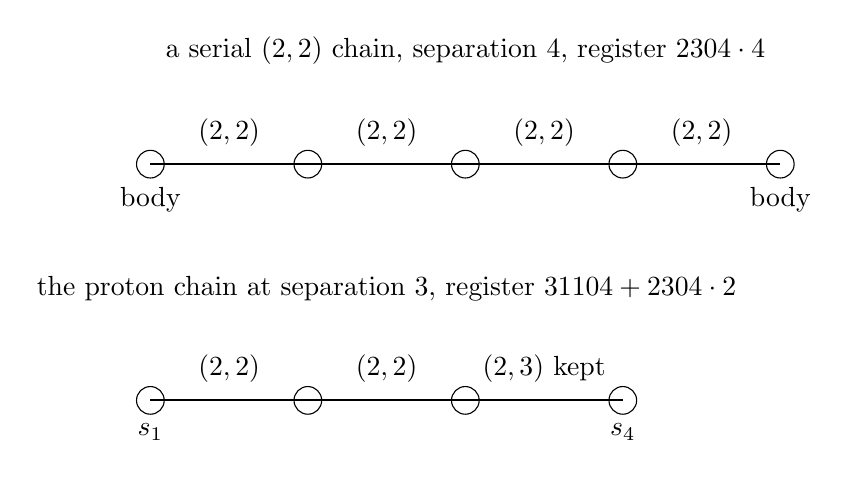
\begin{tikzpicture}[scale=1]
\foreach \x in {0,2,4,6,8} {\filldraw[fill=white] (\x,0) circle (5pt);}
\draw[thick] (0,0) -- (8,0);
\node at (0,0) [below=5pt] {body}; \node at (8,0) [below=5pt] {body};
\node at (1,0) [above=3pt] {$(2,2)$}; \node at (3,0) [above=3pt] {$(2,2)$}; \node at (5,0) [above=3pt] {$(2,2)$}; \node at (7,0) [above=3pt] {$(2,2)$};
\node at (4,1) [above=4pt] {a serial $(2,2)$ chain, separation $4$, register $2304\cdot 4$};
\foreach \x in {0,2,4,6} {\filldraw[fill=white] (\x,-3) circle (5pt);}
\draw[thick] (0,-3) -- (6,-3);
\node at (0,-3) [below=5pt] {$s_1$}; \node at (6,-3) [below=5pt] {$s_4$};
\node at (1,-3) [above=3pt] {$(2,2)$}; \node at (3,-3) [above=3pt] {$(2,2)$}; \node at (5,-3) [above=3pt] {$(2,3)$ kept};
\node at (3,-2) [above=4pt] {the proton chain at separation $3$, register $31104 + 2304\cdot 2$};
\end{tikzpicture}\caption{A serial (2,2) chain between two bodies, whose register is a multiple of the separation, and the chain of the proton sink, whose (2,3) link adds a constant.}\end{figure}
\end{chproof}
\begin{figure}[htbp]\centering
\setlength{\unitlength}{1mm}
\begin{picture}(164,61)(0,0)
\put(8,6){\line(1,0){146}}
\put(10,6){\framebox(4,2){}}\put(15,6){\rule{4mm}{27mm}}\put(14,2){\makebox(0,0){\tiny 1}}
\put(22,6){\framebox(4,4){}}\put(27,6){\rule{4mm}{29mm}}\put(26,2){\makebox(0,0){\tiny 2}}
\put(34,6){\framebox(4,6){}}\put(39,6){\rule{4mm}{31mm}}\put(38,2){\makebox(0,0){\tiny 3}}
\put(46,6){\framebox(4,8){}}\put(51,6){\rule{4mm}{33mm}}\put(50,2){\makebox(0,0){\tiny 4}}
\put(58,6){\framebox(4,10){}}\put(63,6){\rule{4mm}{35mm}}\put(62,2){\makebox(0,0){\tiny 5}}
\put(70,6){\framebox(4,12){}}\put(75,6){\rule{4mm}{37mm}}\put(74,2){\makebox(0,0){\tiny 6}}
\put(82,6){\framebox(4,14){}}\put(87,6){\rule{4mm}{39mm}}\put(86,2){\makebox(0,0){\tiny 7}}
\put(94,6){\framebox(4,16){}}\put(99,6){\rule{4mm}{41mm}}\put(98,2){\makebox(0,0){\tiny 8}}
\put(106,6){\framebox(4,18){}}\put(111,6){\rule{4mm}{43mm}}\put(110,2){\makebox(0,0){\tiny 9}}
\put(118,6){\framebox(4,20){}}\put(123,6){\rule{4mm}{45mm}}\put(122,2){\makebox(0,0){\tiny 10}}
\put(130,6){\framebox(4,22){}}\put(135,6){\rule{4mm}{47mm}}\put(134,2){\makebox(0,0){\tiny 11}}
\put(142,6){\framebox(4,24){}}\put(147,6){\rule{4mm}{49mm}}\put(146,2){\makebox(0,0){\tiny 12}}
\end{picture}

\scriptsize
\setlength{\tabcolsep}{3pt}
\begin{adjustbox}{max width=\linewidth}\begin{tabular}{rllrr}
separation & the element at the pure chains & the element at the carrier chains & register pure & register carrier \\ \hline
1 & 5/384, 5/384, 0, 0 & 79/31104, 1/648, 7/5184, 1/10368 & 2304 & 31104 \\
2 & 5/768, 5/768, 0, 0 & 79/33408, 1/696, 7/5568, 1/11136 & 4608 & 33408 \\
3 & 5/1152, 5/1152, 0, 0 & 79/35712, 1/744, 7/5952, 1/11904 & 6912 & 35712 \\
4 & 5/1536, 5/1536, 0, 0 & 79/38016, 1/792, 7/6336, 1/12672 & 9216 & 38016 \\
5 & 1/384, 1/384, 0, 0 & 79/40320, 1/840, 1/960, 1/13440 & 11520 & 40320 \\
6 & 5/2304, 5/2304, 0, 0 & 79/42624, 1/888, 7/7104, 1/14208 & 13824 & 42624 \\
7 & 5/2688, 5/2688, 0, 0 & 79/44928, 1/936, 7/7488, 1/14976 & 16128 & 44928 \\
8 & 5/3072, 5/3072, 0, 0 & 79/47232, 1/984, 7/7872, 1/15744 & 18432 & 47232 \\
9 & 5/3456, 5/3456, 0, 0 & 79/49536, 1/1032, 7/8256, 1/16512 & 20736 & 49536 \\
10 & 1/768, 1/768, 0, 0 & 79/51840, 1/1080, 7/8640, 1/17280 & 23040 & 51840 \\
11 & 5/4224, 5/4224, 0, 0 & 79/54144, 1/1128, 7/9024, 1/18048 & 25344 & 54144 \\
12 & 5/4608, 5/4608, 0, 0 & 79/56448, 1/1176, 1/1344, 1/18816 & 27648 & 56448 \\
\end{tabular}\end{adjustbox}

\scriptsize the open bar the register at the five pure chains (the electron, muon, tau and neutron webs and the universe web) and the filled bar at the two carrier chains (the proton sink and the photon word), one unit per 1152; the ratio of successive elements as the rows print it, at the pure chains 1/2 at 2, 2/3 at 3, 3/4 at 4, 4/5 at 5, 5/6 at 6, 6/7 at 7, 7/8 at 8, 8/9 at 9, 9/10 at 10, 10/11 at 11, 11/12 at 12 and at the carrier chains 27/29 at 2, 29/31 at 3, 31/33 at 4, 33/35 at 5, 35/37 at 6, 37/39 at 7, 39/41 at 8, 41/43 at 9, 43/45 at 10, 45/47 at 11, 47/49 at 12; the first-power law at the shifted origin 25 over 2 at the carrier chains and at the origin zero at the pure chains.
\caption{The two-point function between the two bodies at the ends of the serial chain at every separation one to twelve, at the five pure chains (the electron, muon, tau and neutron webs and the universe web, each at a (2,2) link) and at the two carrier chains (the proton sink and the photon word, each at a (2,3) link): the element over its register, the register 2304 multiplied by the separation at the pure chains and 31104 plus 2304 multiplied by the separation less one at the carrier chains, the first-power law at the shifted origin 25 over 2. The bars are the registers at one unit per 1152, no fitted curve.}\label{fig:V-11-D543290-two-point-function}
\end{figure}
\par\medskip\noindent{\itshape One relation among the three charged leptons closes the Part.}\label{narr:close:5-11}\par
\section{The Koide class}\label{mod:V-12-koide-class}
\chdesig{7-12}{5-12}{V-12-koide-class}{V-12-koide-class}
\label{narr:open:5-12}Open result~157.1 states the Koide relation at the dock unit as an open result, resting on the mass unit, the lepton ladder and the next terms of chapter 8-3.
\begin{chwall}[The Koide relation at the dock unit]\label{box:V-12-koide-class:1}
At the dock spelling with the electron at its dock-struck first power in place of the hub first power, the relation lies outside the field of the two roots at the direct-sum order, the three adjoined roots independent, so it equals two thirds in the field at no reading, the departure an exact object of the tower with the sign positive at the ladder of the construction and negative at the derived ladder, both faces printed at every cell.
Open are the two results above, the relation undefined at a surd at the direct-sum order and departing from two thirds at the dock unit at every reading; the standing placement is the link weight, a choice we made, and the next term at that placement for the three leptons stands at its own chapter of Part VII. Re-posed at a second route at the order-two read through the hub: every reading of the relation at the dock spelling re-derived from the primary tables alone equals the first route at twenty-seven of twenty-seven readings, the six readings at the dock spelling at six of six, the first parting standing; at the cell of reference, the catalogue ladder at the link-weight placement and the direct-sum order, the dock-spelled direct sum of the electron re-met by value is no square in the field of root two and root three at the second route through the subfield of root three and the subfield of root six, so the relation lies outside the field at both routes, the roots in the field none of three and independent; the departure from two thirds at that cell is positive at the second route with its sixty-digit bracket consistent with the forty-digit bracket of the first, the next term negative and consistent alike, the first-order relation at the dock spelling 16684819 over 24990001 with the departure 74455 over 74970003 positive at both routes; the hub-spelling readings, negative at every reading, and the derived-ladder readings are equal at both routes and printed beside.
\end{chwall}
\chstanding{an open result}
\chdeps{Definitions 1.1 to 1.6, Theorem 152.1, Theorems 185.1 to 185.12 and Theorems 196.1 and 196.2}{no theorem beyond it at this release}
At the deciding reading of the ladder of the construction, the link-weight placement and the direct sum as the mass, the three charged-lepton direct sums are exact nonzero elements of the field of the two roots and the root of every one of the three lies outside that field, decided exactly through the subfield of the first root, so the relation at the direct-sum order is undefined at a surd in the field the sums live in, the next term an exact object of the formal tower with its sign negative at the standing placement, printed for the comparison table alone.
\begin{chbridge}
The Koide relation states that the sum of the three charged-lepton masses divided by the square of the sum of their square roots is two thirds, an empirical relation holding to high accuracy and derived from no principle of the Standard Model \cite{Koide1983}; it is a statement about the three masses as one triple and no statement about any one of them. The correspondence is by name; the record supplies an isometry algebra of the Hermitian split at the Lorentz brackets, a lattice point group, boosts from the order register and a transverse traceless part at the open read, every one a finite or algebraic object of this theory carrying the group name at chapter~\ref{mod:III-2-rotation-group}, chapter~\ref{mod:III-3-lorentz-group-and-the-signature}, chapter~\ref{mod:III-4-boosts-and-the-one-unit}, chapter~\ref{mod:III-5-spin-and-helicity}, the chapter titled Causal structure and general covariance (chapter~\ref{mod:III-8-causal-structure-and-general-covariance}, among the instruments) and chapter~\ref{mod:XIV-7-what-remains-the-ungraded-page}, and the mass corresponds there and here by name.
\end{chbridge}
\begin{chproof}[exact]
The premises of this derivation are the axiom and the six definitions of chapter~\ref{mod:FRAMEWORK}, the theorem of chapter~\ref{mod:VIII-1-mass-unit-and-the-first-power}, the theorem of chapter~\ref{mod:V-10-lepton-ladder-as-hub-assemblies} and the theorem of chapter~\ref{mod:VIII-3-next-terms-and-the-unstable-rows}. The chain of premises runs back to the axiom through those chapters, and the longest such chain in this compendium is twelve chapters long.
This chapter carries no theorem and states its two open results: the three direct sums are taken at the direct-sum order at the ladder of the construction and the link-weight placement (the placement), their roots tested exactly for membership in the field of the two roots through the subfield of the first root, and the relation evaluated at the dock unit at every standing reading, the departure an exact object of the formal tower of the three adjoined roots, every cell compared with nothing on this page.
From the ladder of the construction at the link-weight placement with the electron at its dock-struck first power sixty-seven in place of the hub first power two hundred and one, by the direct sum at the direct-sum order, we obtain the three charged-lepton direct sums as exact nonzero elements of the field of the two roots. At the electron the dock-spelled sum is the hub-spelled sum over the factor nine,
\begin{equation}
\Sigma_{e}^{\mathrm{dock}} = \frac{2\ 144\ 666\ 856\ 770\ 839}{477\ 757\ 440\ 000} + \frac{661}{36450}\sqrt{2} + \frac{5\ 977\ 541}{23\ 887\ 872\ 000}\sqrt{3} = \frac{\Sigma_{e}^{\mathrm{hub}}}{9} ,
\end{equation}
and from the three dock-spelled sums, by the exact test of membership of their roots in the field through the subfield of the first root, we obtain that none of the three roots lies in the field, the three adjoined roots independent, so the relation lies outside the field and equals two thirds in the field at no reading, the electron the first parting.
\begin{equation}
\sqrt{\Sigma_{\ell}} \notin \mathbb{Q}(\sqrt{2}, \sqrt{3}) \quad \text{for } \ell = e, \mu, \tau, \qquad \frac{\Sigma_{e} + \Sigma_{\mu} + \Sigma_{\tau}}{(\sqrt{\Sigma_{e}} + \sqrt{\Sigma_{\mu}} + \sqrt{\Sigma_{\tau}})^{2}} \ne \tfrac{2}{3} \ \text{in the field} .
\end{equation}
From the first-order relation at the dock spelling, by exact rational arithmetic, we obtain its departure from two thirds as a positive rational, and at the hub spelling a negative one, the sign of the departure of the relation itself and of its next term certified at the dock spelling by exact brackets at forty digits, positive and negative.
\begin{equation} \adjustbox{max width=\dimexpr\linewidth-3em\relax}{$\displaystyle \begin{gathered} K_{1}^{\mathrm{dock}} = \frac{16\,684\,819}{24\,990\,001}, \quad K_{1}^{\mathrm{dock}} - \tfrac{2}{3} = \frac{74\,455}{74\,970\,003} > 0; \\ K_{1}^{\mathrm{hub}} = \frac{1\,857\,859}{2\,927\,521}, \quad K_{1}^{\mathrm{hub}} - \tfrac{2}{3} = -\frac{281\,465}{8\,782\,563} < 0 . \end{gathered}$} \end{equation}
The counter-tests of the entry alter the objects singly and read what moves, every one at its pinned letter at both engines, the hub-spelling cells of the preceding result re-met by value at all four direct-sum cells and both first-order cells, and every sign certified by an exact bracket at forty digits at all eight cells. The result was reproduced by a second engine built apart from the first, the two runs byte-identical at every piece with no differing shared key. The departure is an exact object of the tower printed for the comparison table alone and no digit of a lepton mass enters here. This result carries its cells in its own statement and at no table of its own, so every quantity above is read from that statement.
The machine-checked package named at the reproducibility appendix certifies the statements of this chapter under the definitions of this compendium.
\end{chproof}
\begin{figure}[h]\centering
\begin{adjustbox}{max width=\linewidth}\begin{tabular}{lll}\hline lepton & first power at the dock spelling & hub assemblies \\ \hline the electron & 67 & 1 \\ the muon & 107 & 2 \\ the tau & 147 & 3 \\ \hline \end{tabular}\end{adjustbox}
\caption{The object of this chapter as a listed table, the three charged leptons of the ladder at the dock spelling, the dock-struck first power of each and its count of hub assemblies, the direct sums of this chapter being formed from these at the direct-sum order.}
\end{figure}
\par\medskip\noindent{\itshape Electrodynamics read, Part VIII turns to the weak interaction.}\label{narr:close:5-12}\par
